\section{Categorization} \label{sec:ttHCPCategorization}

In order to properly measure the dependence of the top Yukawa coupling on the CP-mixing angle $\alpha$, a region of $ttH$-and-$tH$-enriched phase space  is divided into a number of different categories based both upon the similarity of events it contains to signal (Higgs processes like $ttH$ and $tH$) rather than background (non-Higgs continuum diphoton processes), as well as the similarity of events it contains to CP-odd rather than CP-even Higgs processes. By creating many such categories and fitting the event yield in each, detailed constraints can be set on the value of $\alpha$.

First, two sets of regions are defined. The "hadronic" region targets events containing fully-hadronic top decays, requiring two loose-ID photons, one b-tagged jet at the 77\% working point with $p_{T} > 25$ GeV, as well as two additional jets with $p_{T} > 25$ GeV and exactly zero electrons or muons. Similarly, the "leptonic" region targets events containing semi-leptonic top decays, requiring two loose-ID photons, one b-tagged jet at the 77\% working point with $p_{T} > 25$ GeV, as well as at least one isolated electron or muon.

To perform the categorization in these regions, two multivariate Boosted Decision Trees (BDTs) are used, one to separate Higgs events from background and one to separate CP-odd Higgs events from CP-even Higgs events. Both BDTs are trained on low-level kinematic features using the XGBoost package \cite{XGBoost}. A series of cuts on these BDT scores are then defined, delineating a total of 20 orthogonal regions, each with differing sensitivity both to the $ttH+tH$ signal and to the CP-odd $ttH+tH$ hypothesis. An illustration of the categorization strategy is shown in figure \ref{fig:cartoon}.

\begin{figure}[htbp]
  \centering
        \subfloat[Hadronic categories]{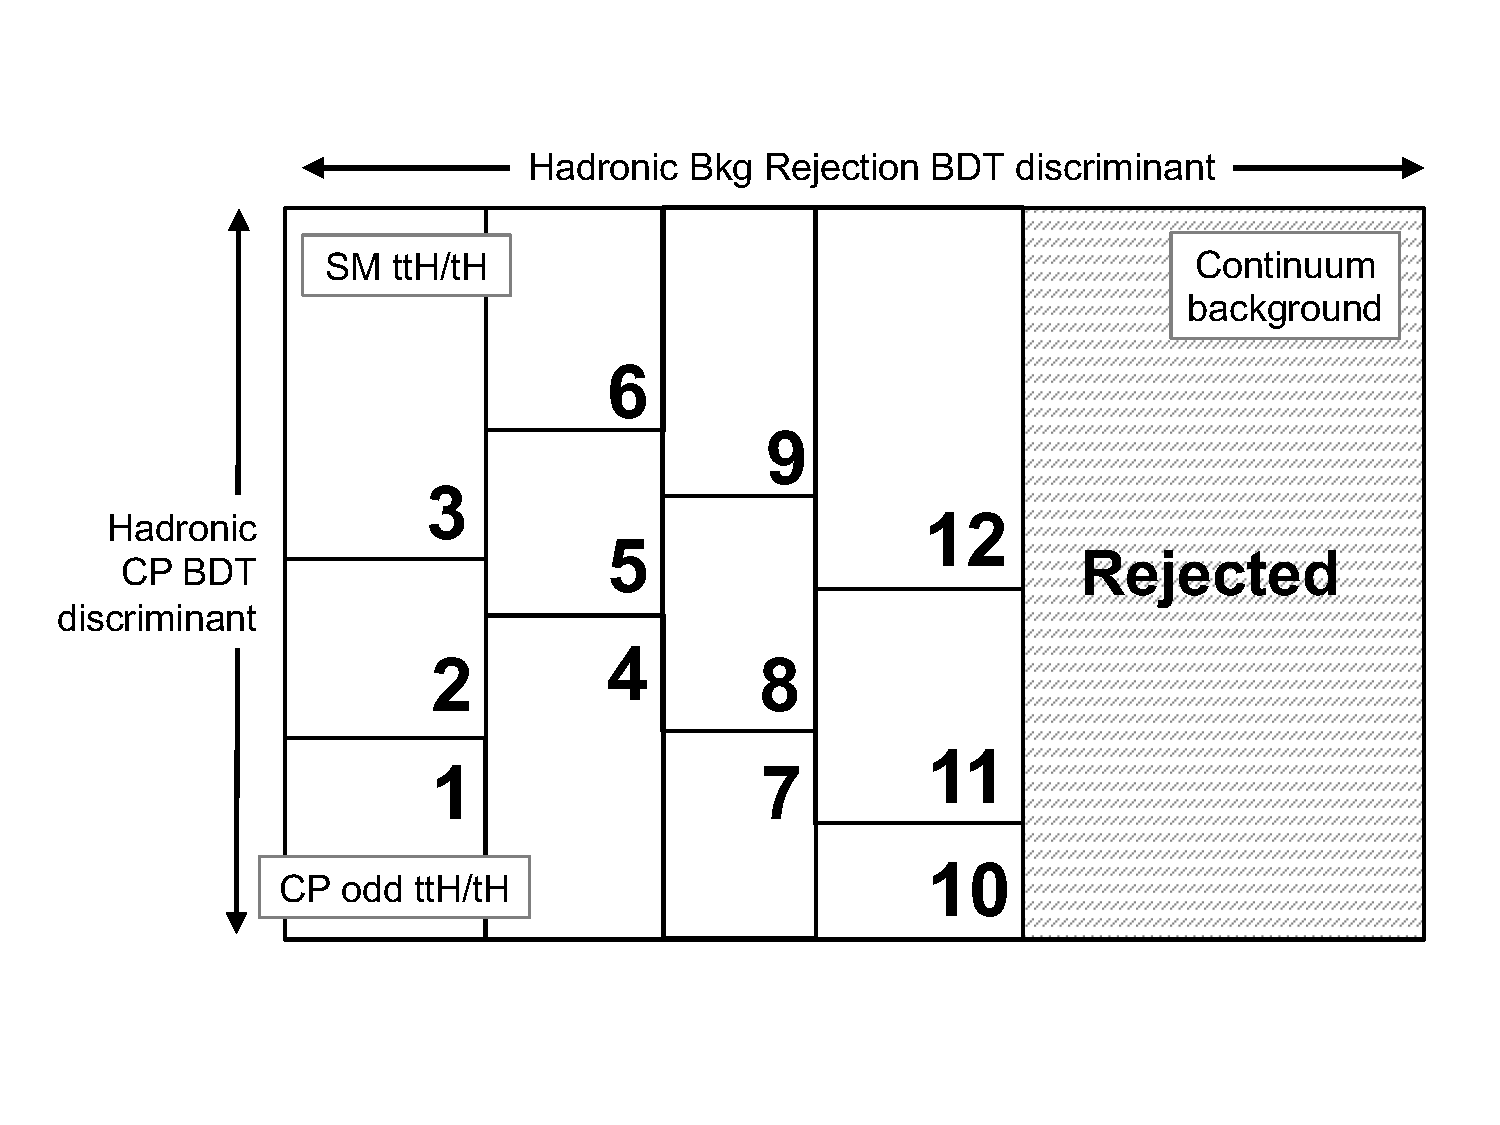
\includegraphics[width=0.42\textwidth]{figures/tthcp_chapter/categorization_xgb/had/grid_had.pdf}}
        \subfloat[Leptonic categories]{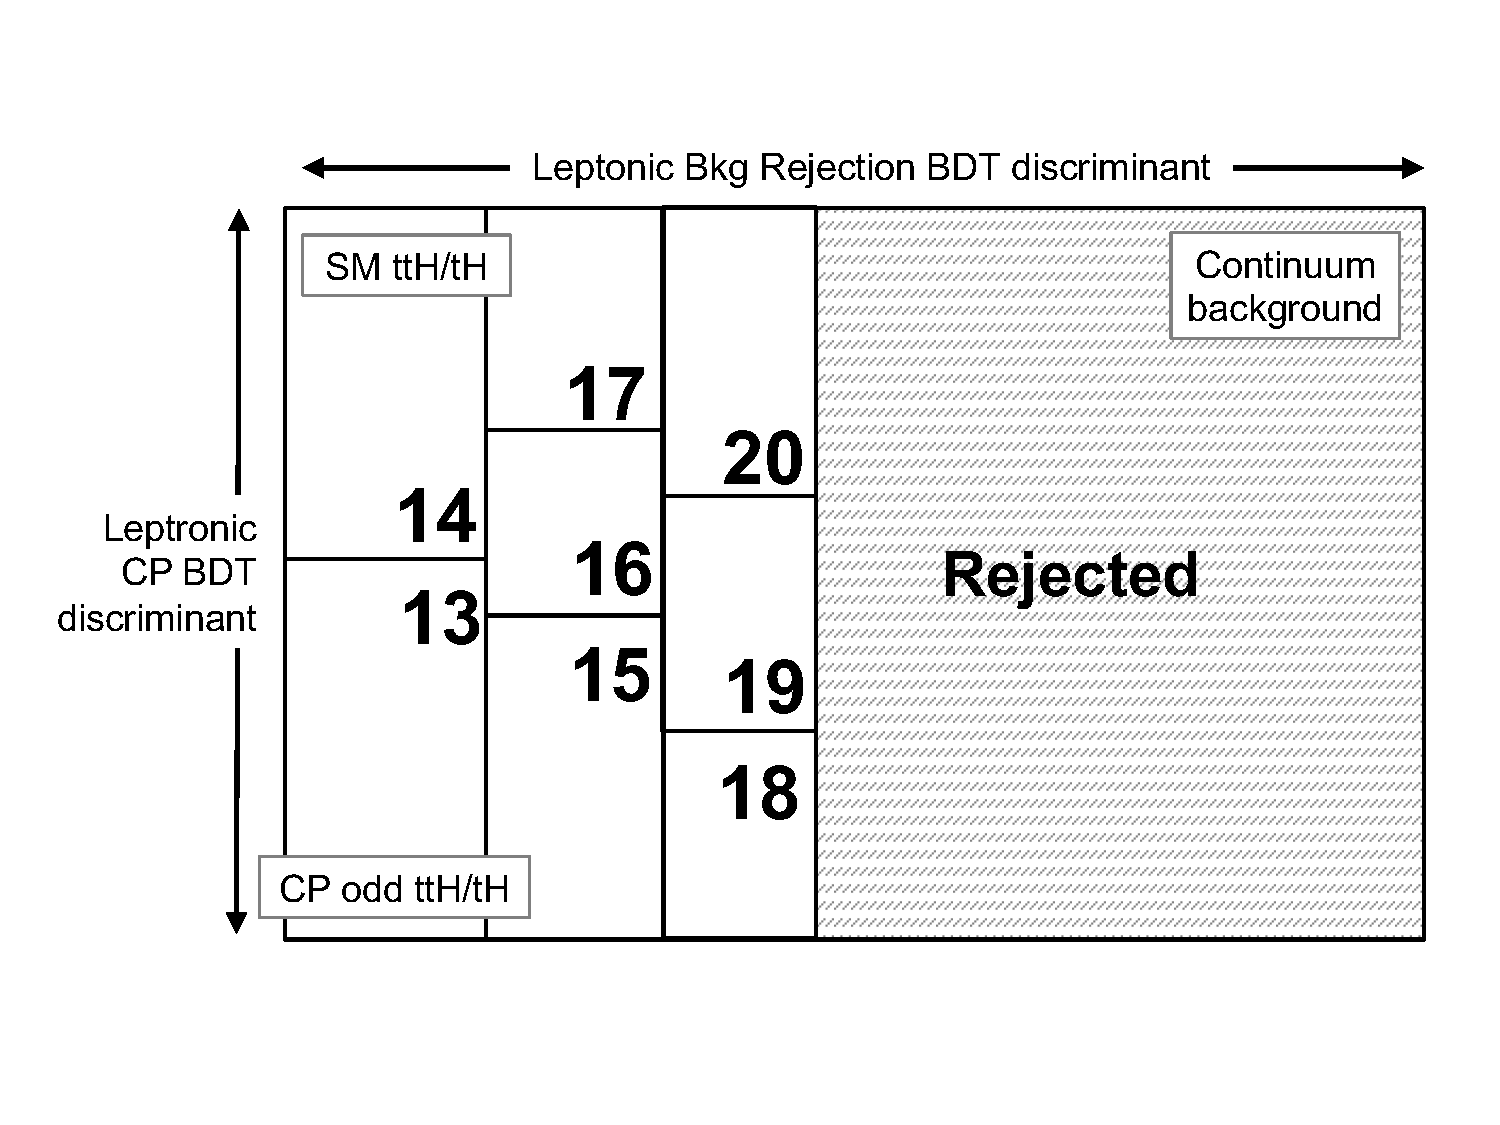
\includegraphics[width=0.42\textwidth]{figures/tthcp_chapter/categorization_xgb/lep/grid_lep.pdf}}
  \caption{Diagram of the 2-dimensional categorization scheme in the hadronic (a) and leptonic (b) channels. The $x$-axis indicates the background-rejection BDT (SBBDT) score distribution, and the $y$-axis represents the CP-BDT score distribution. The shaded region indicates rejected events.}
  \label{fig:cartoon}
\end{figure}

\subsection{SBBDT}

The signal-versus-background BDT (SBBDT) developed for use in the CP Analysis is identical to that developed first in the $79.8 fb^{-1}$ measurements of $ttH$ in the diphoton channel \cite{ttH} in and later retrained for $139 fb^{-1}$ measurements of $ttH$ in the diphoton channel \cite{ATLAS-CONF-2019-004}. It is trained separately for both the hadronic and leptonic regions.

Both the hadronic and leptonic BDTs are trained using a Standard-Model Powheg $ttH$ Monte Carlo sample to model the signal and NTI data control events to model the continuum diphoton background.

\subsubsection{Hadronic Region} \label{sec:SBBDThad} 
In the hadronic region, 60\% of the $ttH$ Monte Carlo signal events are used for training, 20\% are reserved for categorization and BDT hyperparameter optimization, and the final 20\% are reserved for validation. 60\% of the NTI events are used for training, 20\% are reserved for hyperparameter optimization, and the remaining 20\% are reserved for testing and significance evaluation.

The input variables chosen are: 

\begin{itemize}
\item $p_{T}/m_{\gamma \gamma}$, $\eta$ and $\phi$ of the two photons. Photon $p_{T}$ is scaled by $m_{\gamma \gamma}$ to reduce unwanted sculpting of the diphoton mass spectrum. 
\item $p_T$, $\eta$, $\phi$ and E of the six highest-$p_{T}$ jets
\item Boolean b-tag value for each of the six highest-$p_{T}$ jets (77\% working point)
\item $E_T^{miss}$ and direction of $E_T^{miss}$
\end{itemize}

Distributions of the BDT input variables using $79.8 fb^{-1}$ of data are shown in Figure \ref{fig:SBBDTvarshad}.

\begin{figure}
	\centering
	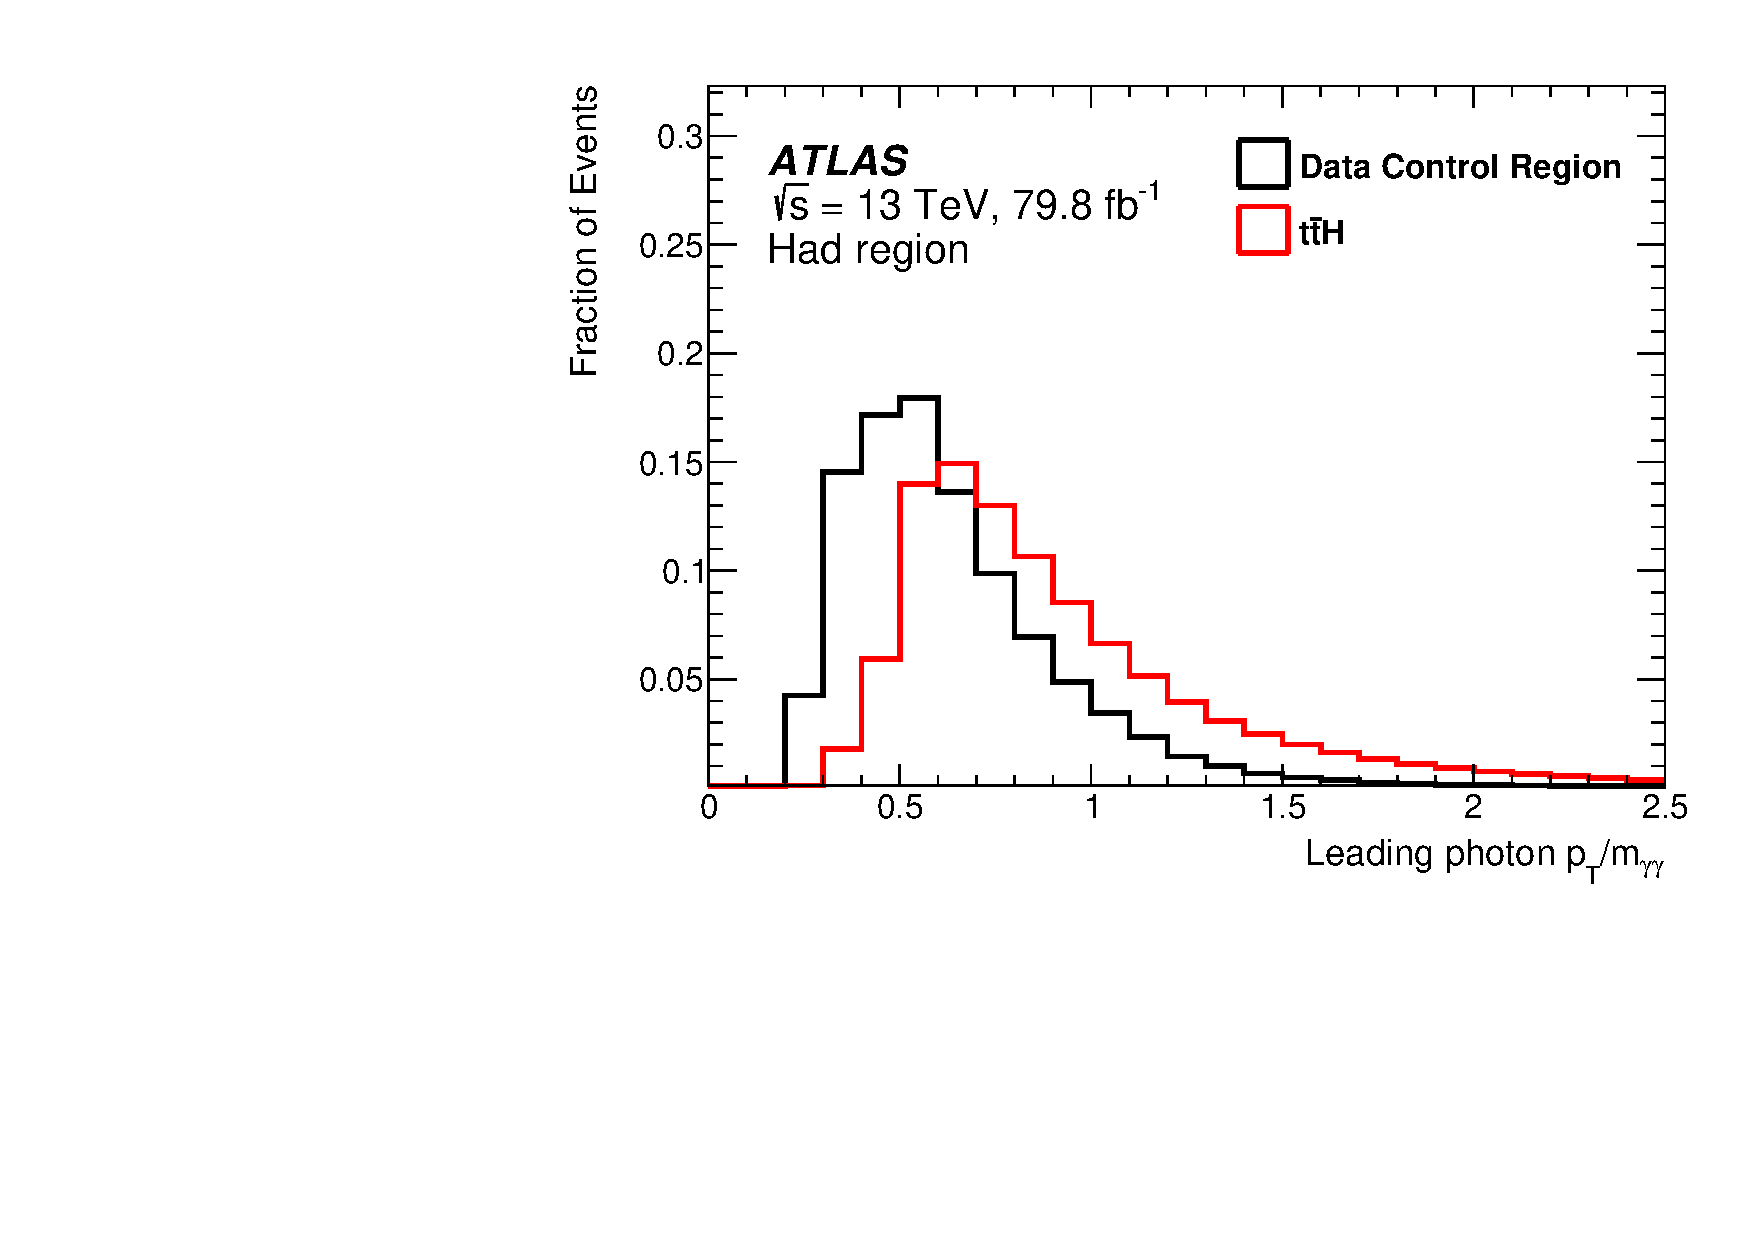
\includegraphics[width=0.31\linewidth]{figures/tthcp_chapter/figaux_10a.pdf}
	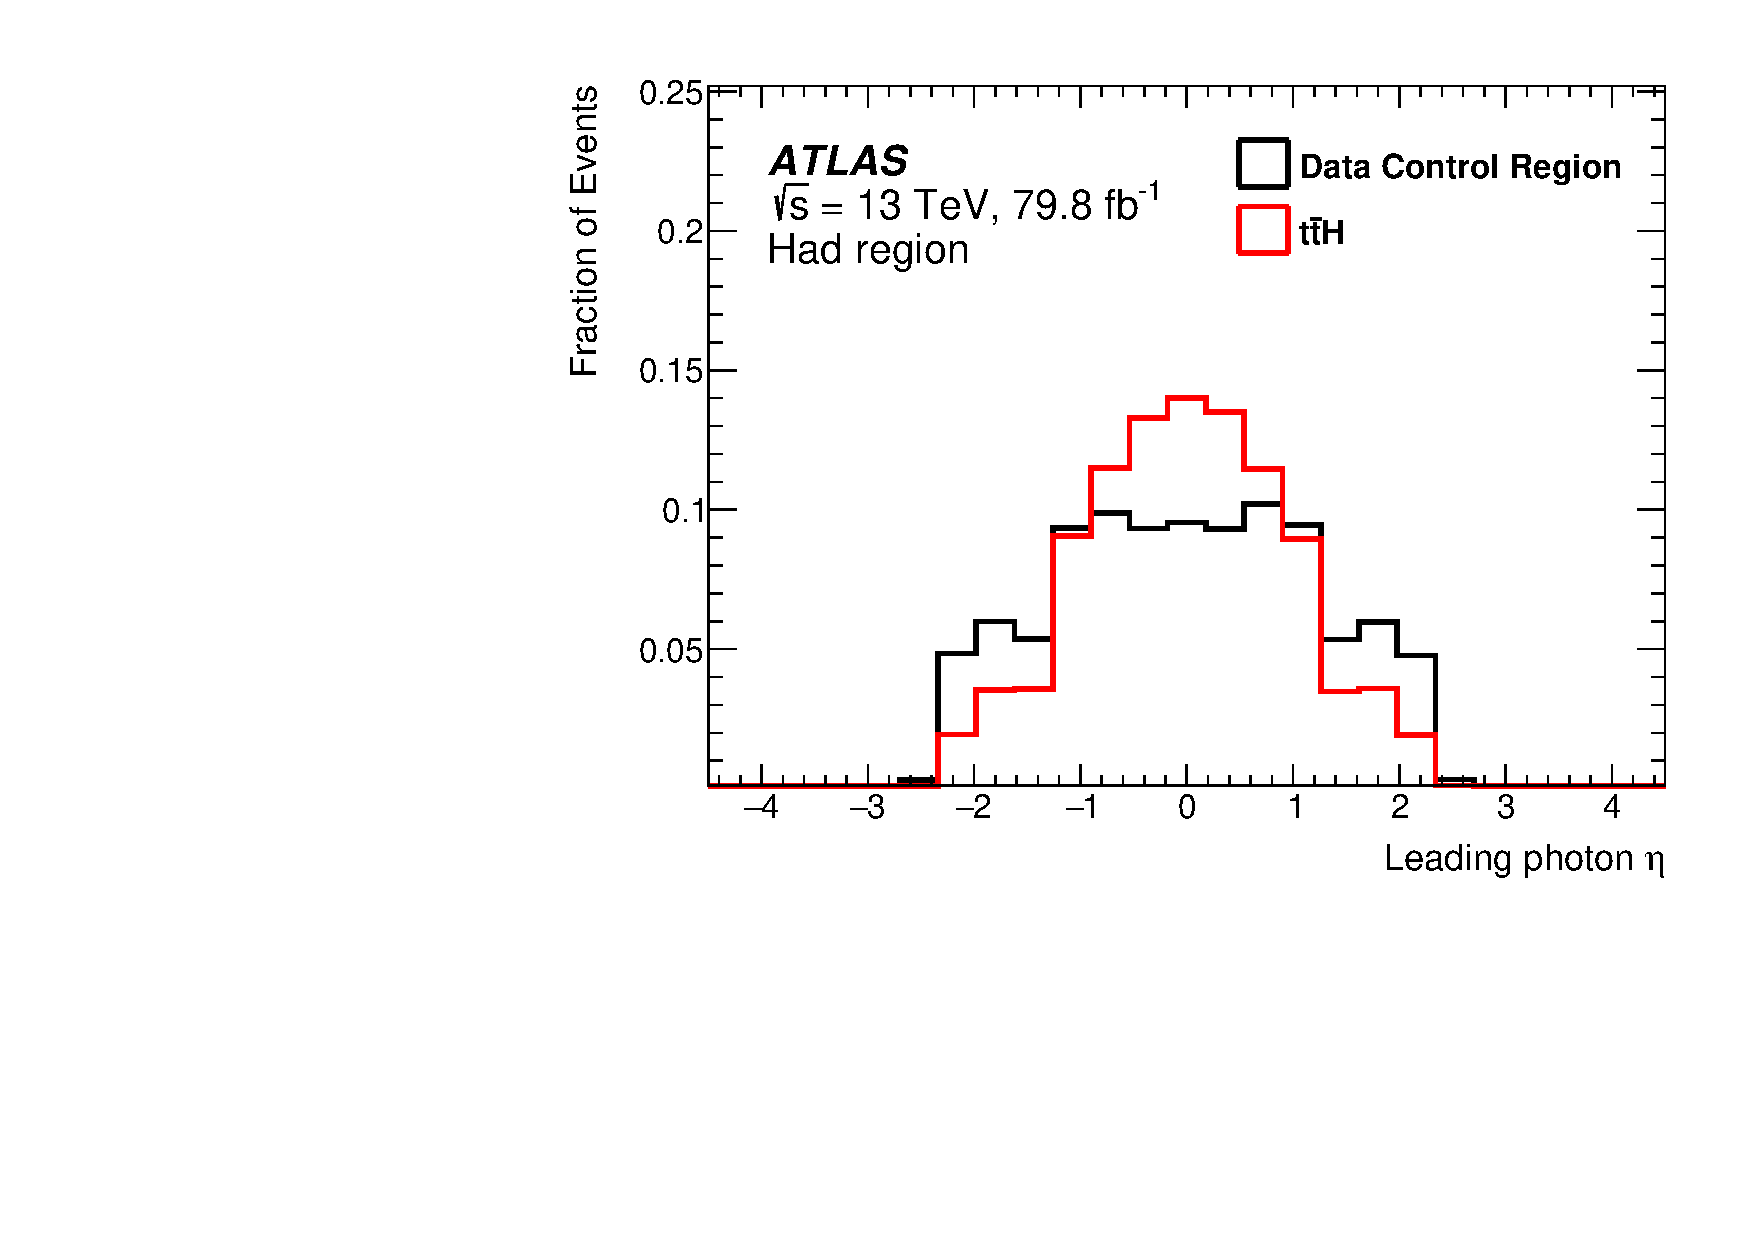
\includegraphics[width=0.31\linewidth]{figures/tthcp_chapter/figaux_10b.pdf}
	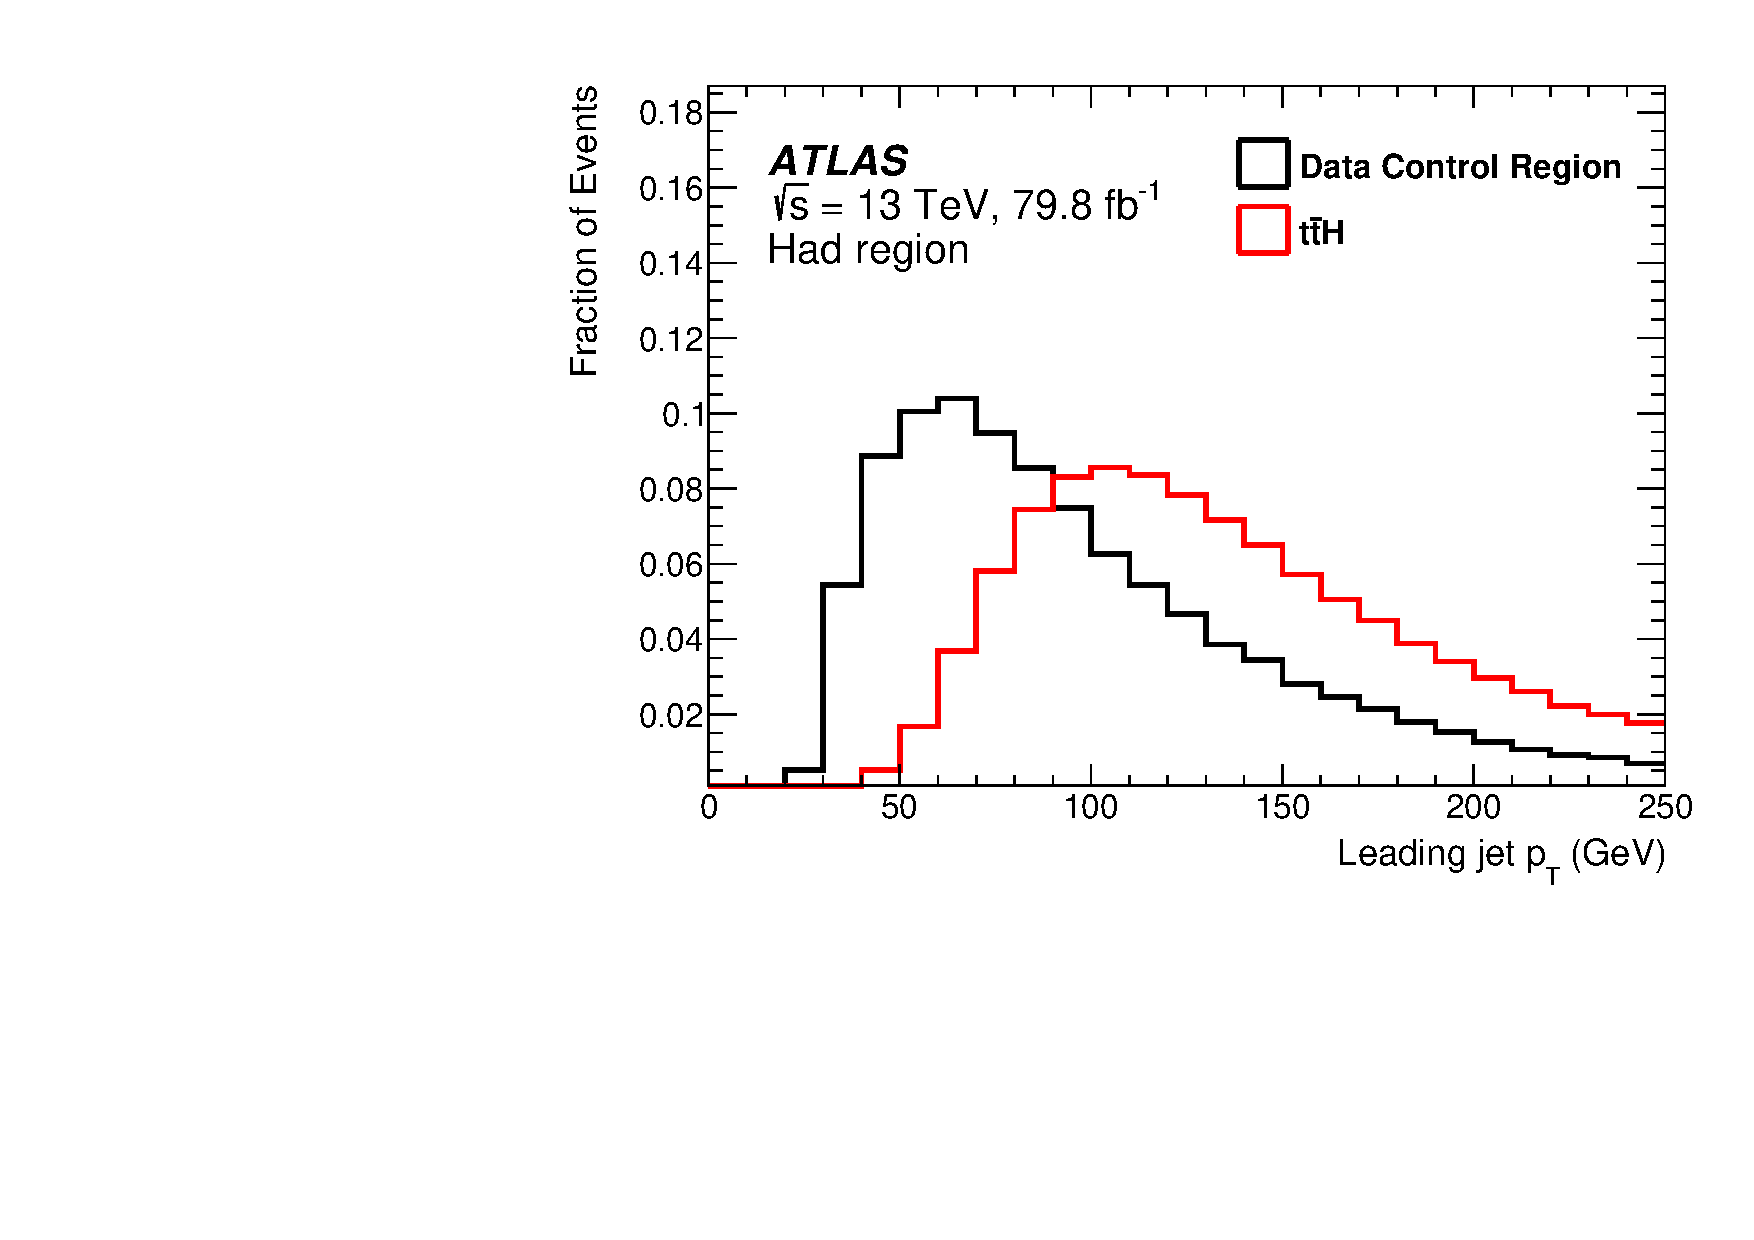
\includegraphics[width=0.31\linewidth]{figures/tthcp_chapter/figaux_10c.pdf}
	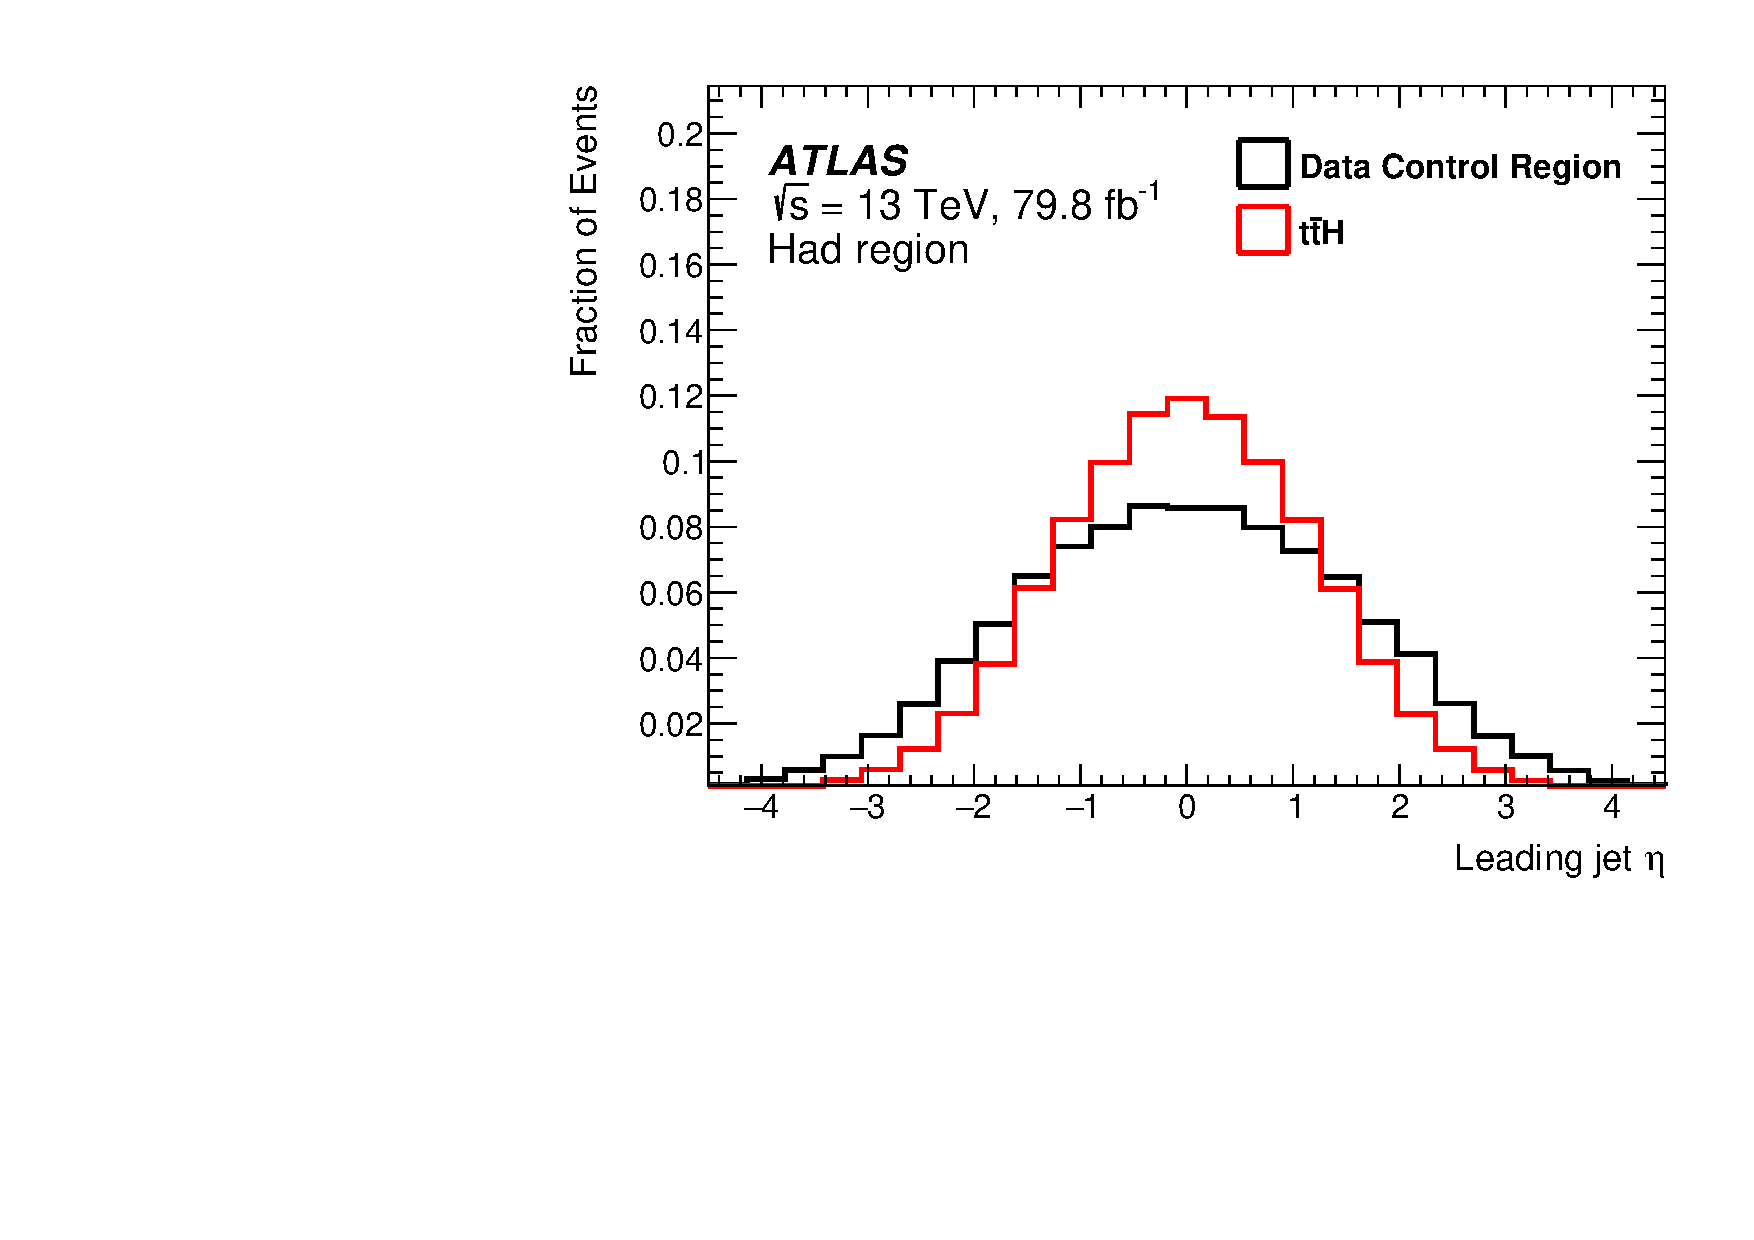
\includegraphics[width=0.31\linewidth]{figures/tthcp_chapter/figaux_10d.pdf}
	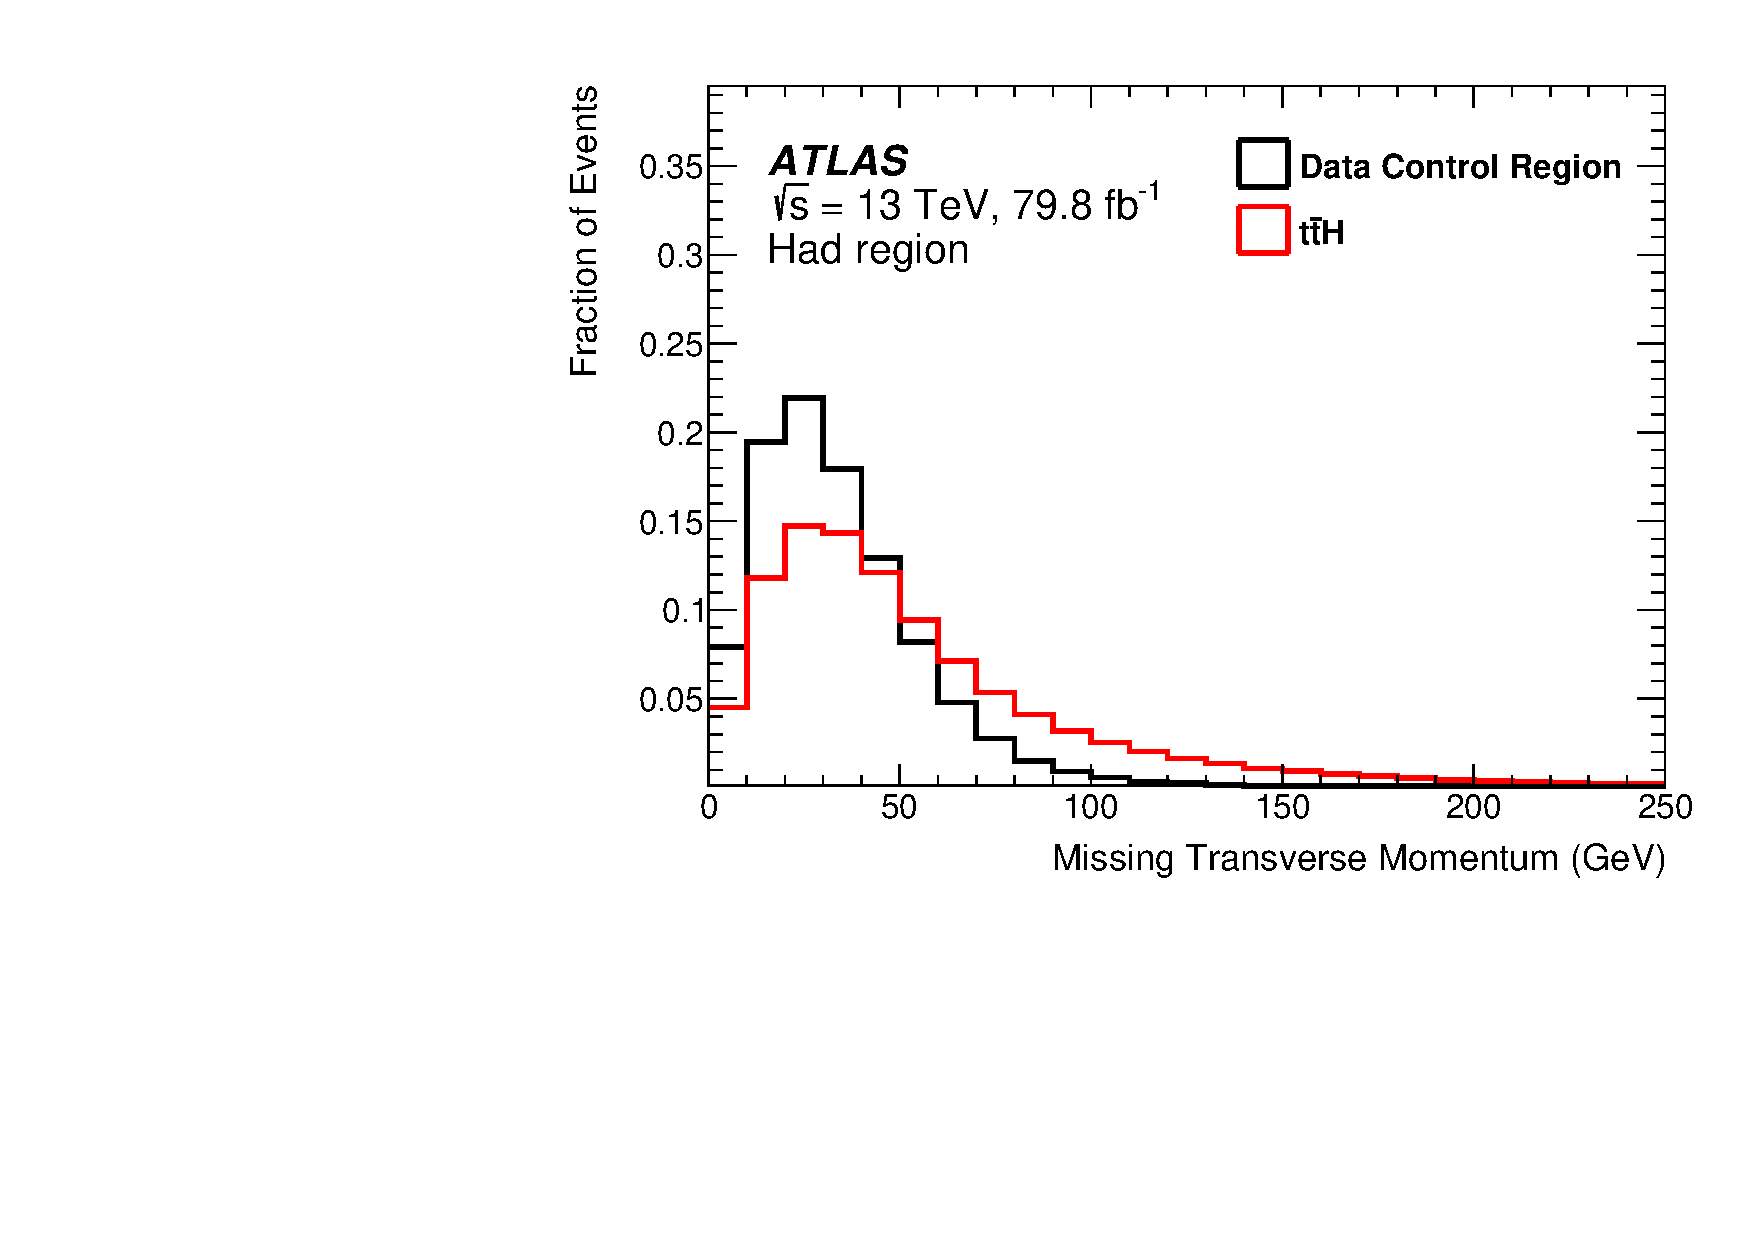
\includegraphics[width=0.31\linewidth]{figures/tthcp_chapter/figaux_10e.pdf}
	\caption{Distributions of training variables for the hadronic background-rejection BDT, trained at $79.8 fb^{-1}$. Taken from \cite{ttH}. }
	\label{fig:SBBDTvarshad}
\end{figure}

\subsubsection{Leptonic Region} \label{sec:SBBDTlep} 

As in the hadronic region, in the leptonic region, 60\% of the $ttH$ Monte Carlo signal events are used for training, 20\% are reserved for categorization and BDT hyperparameter optimization, and the final 20\% are reserved for validation. 75\% of the NTI events containing zero b-jets but at least one un-tagged jet wiare used for training and the remaining 25\% are reserved for hyperparameter optimization, while 50\% of the NTI events containing one or more b-jets are used for categorization and the remaining 50\% are reserved for testing and significance evaluation.

However, due to lower statistics in the leptonic top decay channel due to the smaller top-quark branching ratio to leptons, two cuts are relaxed for the development of the leptonic BDT:

\begin{itemize}
\item The relative $p_{T}$ cuts are loosened from $\frac{p_{T}}{m_{\gamma\gamma}} > 0.35$ for the leading photon and $\frac{p_{T}}{m_{\gamma\gamma}} > 0.25$ for the subleading photon to a flat $p_{T} > 35$ GeV for the leading photon and $p_{T} > 25$ GeV for the subleading photon.
\item The diphoton invariant mass window is extended from $105$ GeV $< m_{\gamma \gamma} < 160$ GeV to $80$ GeV $< m_{\gamma \gamma} < 250$ GeV.
\end{itemize}

The cuts are again tightened to define the signal region after BDT training is complete- that is, the loosening of these cuts is only utilized to increase BDT training statistics, and does not carry through to other stages of the analysis.

The input variables chosen are: 

\begin{itemize}
\item $p_T/m_{\gamma \gamma}$, $\eta$ and $\phi$ of the two photons. Photon $p_{T}$ is scaled by $m_{\gamma \gamma}$ to reduce unwanted sculpting of the diphoton mass spectrum.
\item $p_T$, $\eta$ and $\phi$ of up to two leptons. 
\item $p_T$, $\eta$, $\phi$ and E of the four jets with highest $p_{T}$
\item Boolean b-tag flag (77\% working point) for each of the four jets with highest $p_{T}$
\item $E_T^{miss}$ and direction of $E_T^{miss}$
\end{itemize}

Distributions of the BDT input variables using $79.8 fb^{-1}$ of data are shown in Figure \ref{fig:SBBDTvarslep}. The BDT output distributions are shown in figures \ref{fig:moriondtotal}. The SBBDT performance is independent of $\alpha$.

\begin{figure}
	\centering
	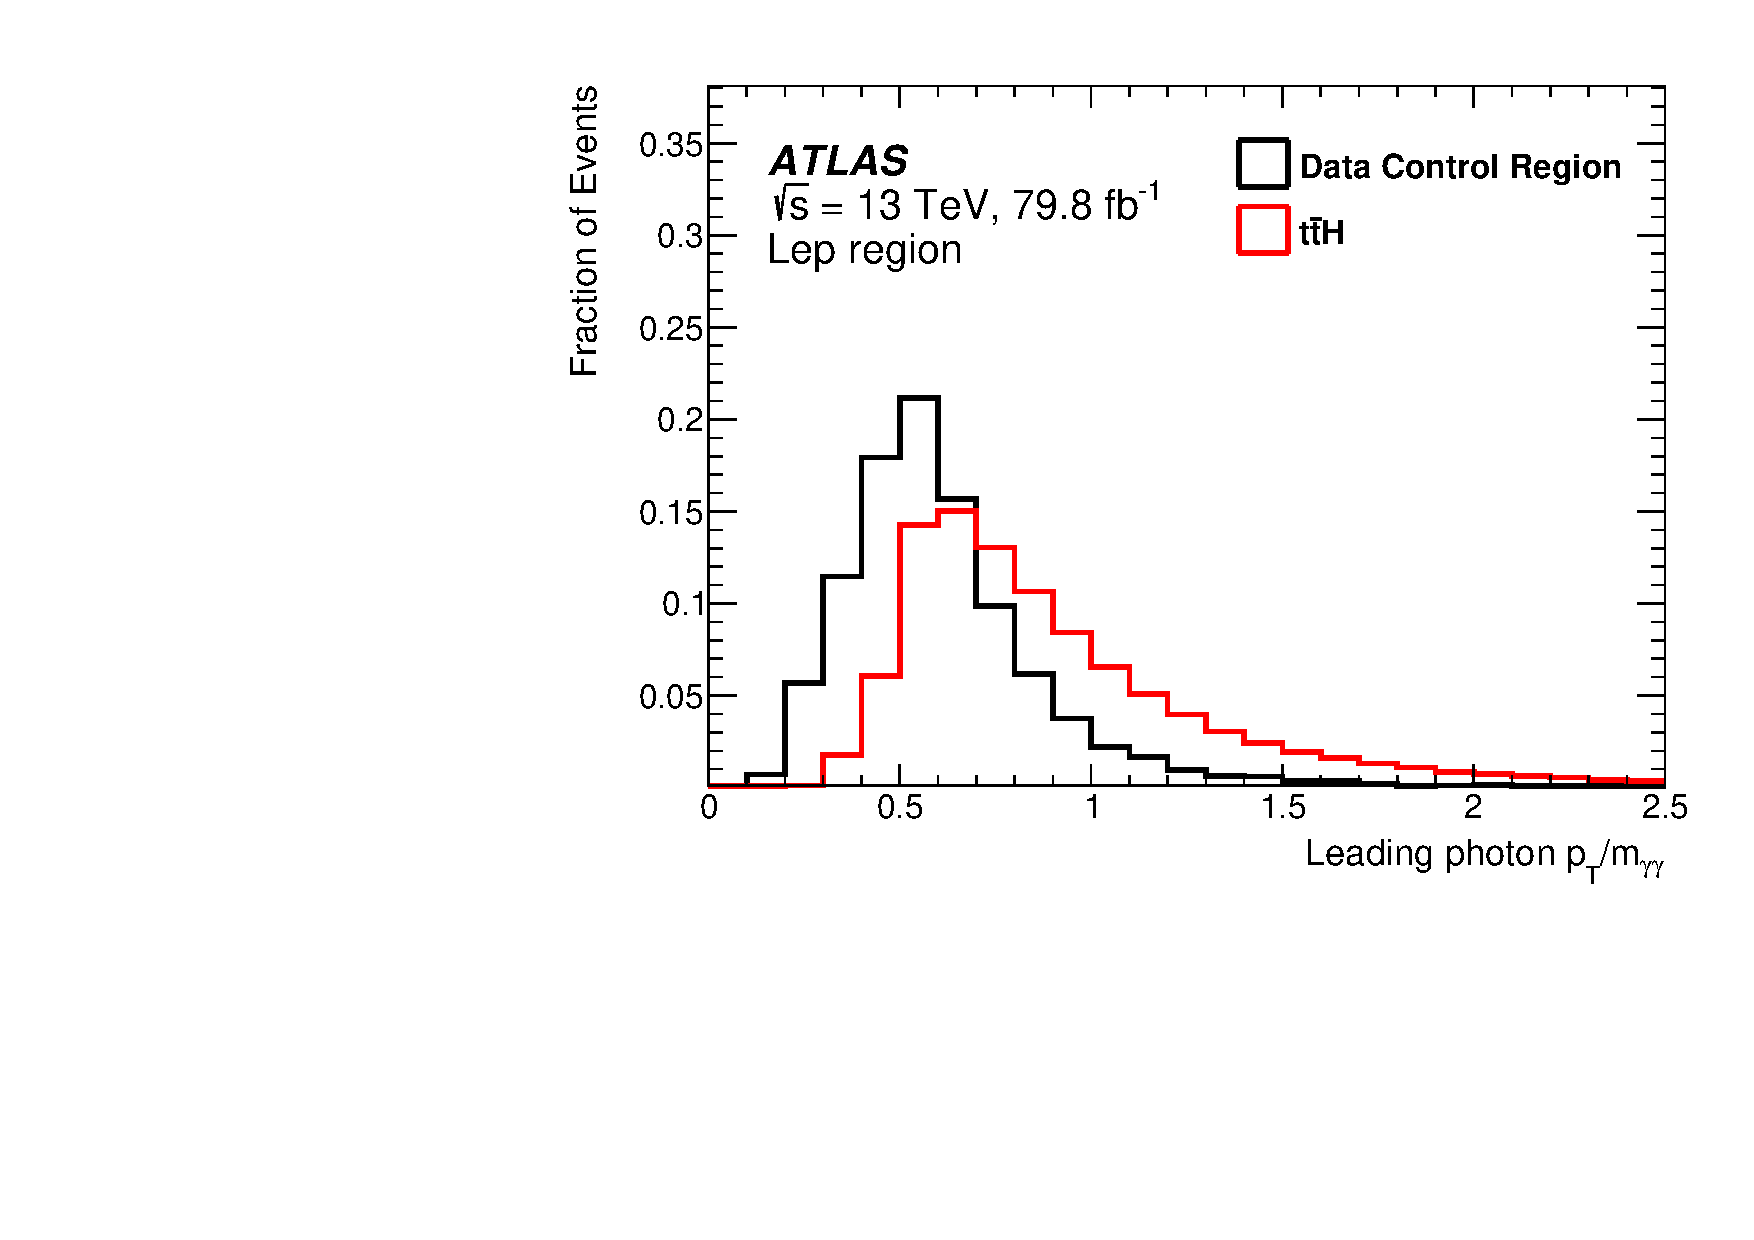
\includegraphics[width=0.31\linewidth]{figures/tthcp_chapter/figaux_11a.pdf}
	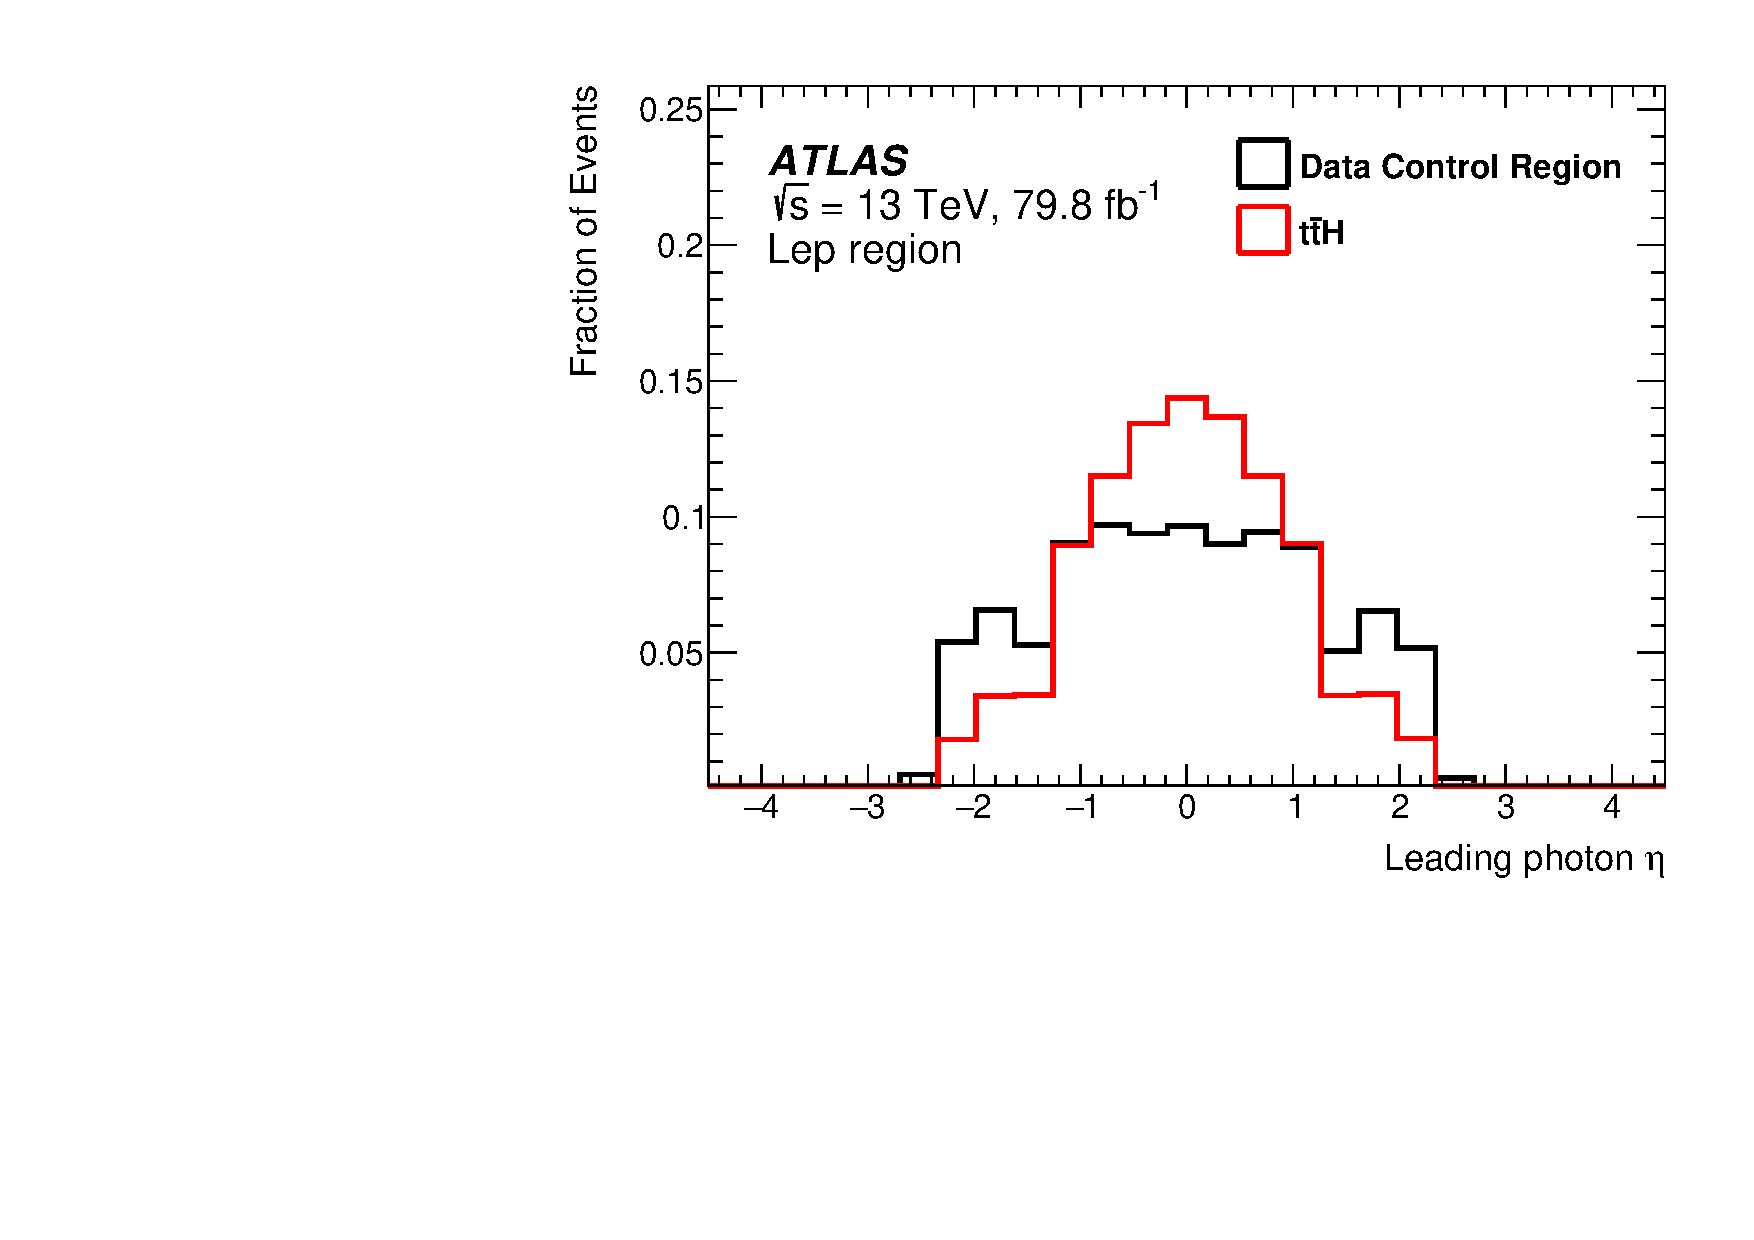
\includegraphics[width=0.31\linewidth]{figures/tthcp_chapter/figaux_11b.pdf}
	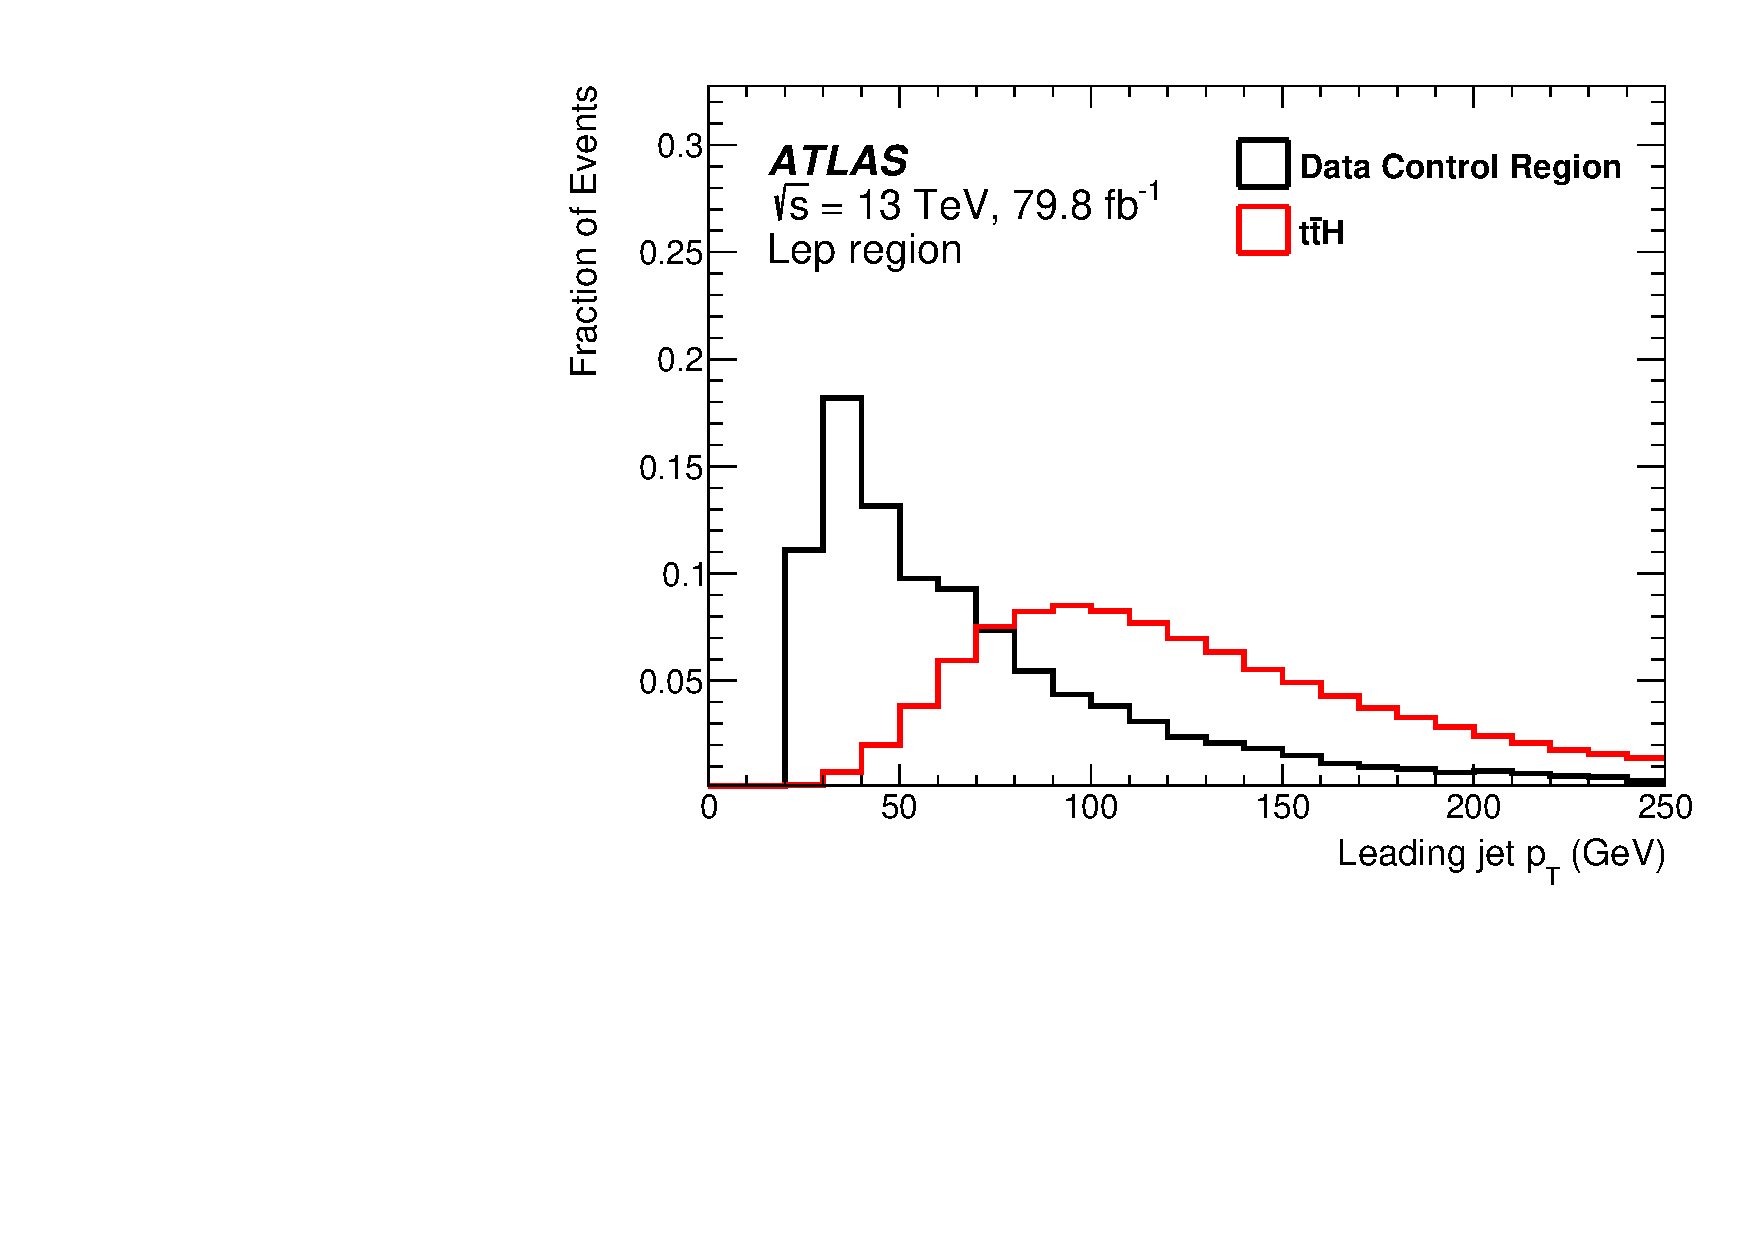
\includegraphics[width=0.31\linewidth]{figures/tthcp_chapter/figaux_11c.pdf}
	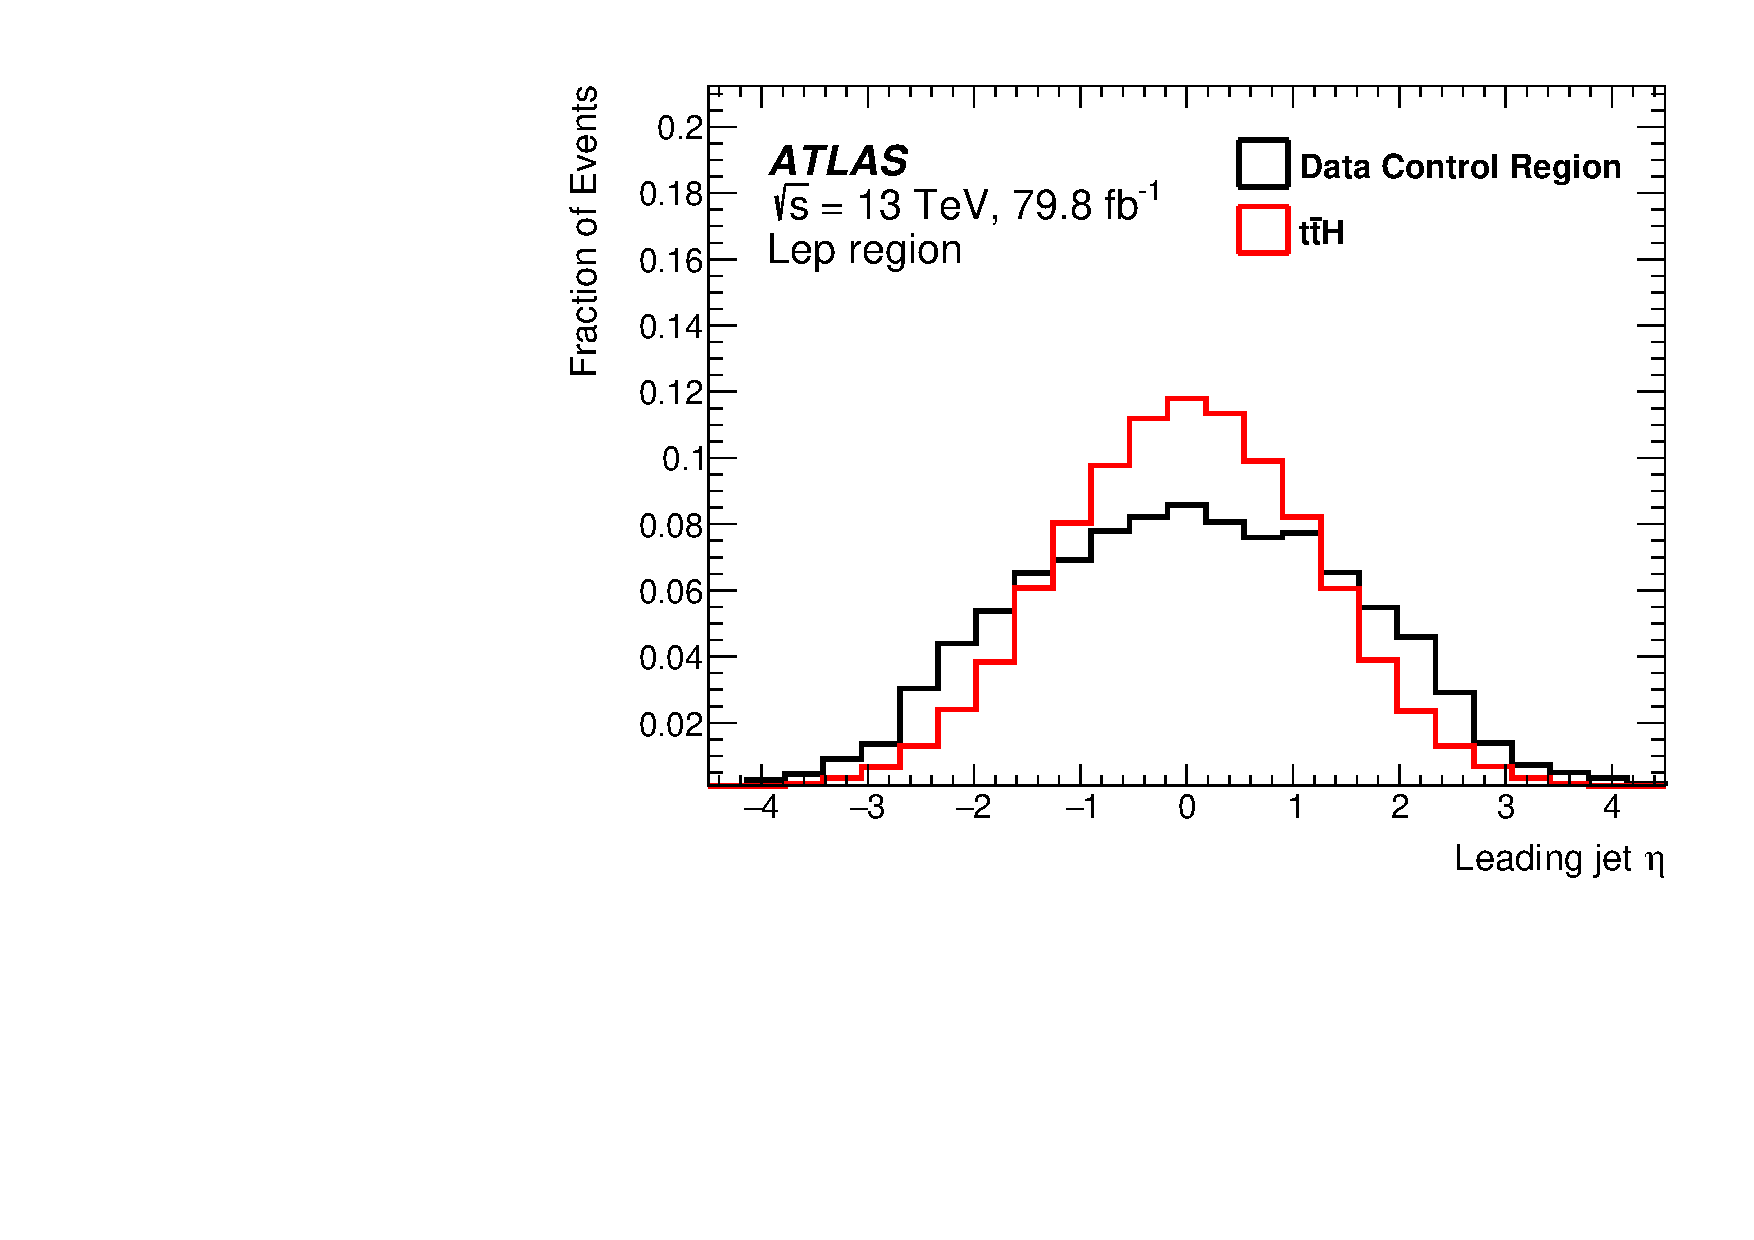
\includegraphics[width=0.31\linewidth]{figures/tthcp_chapter/figaux_11d.pdf}
	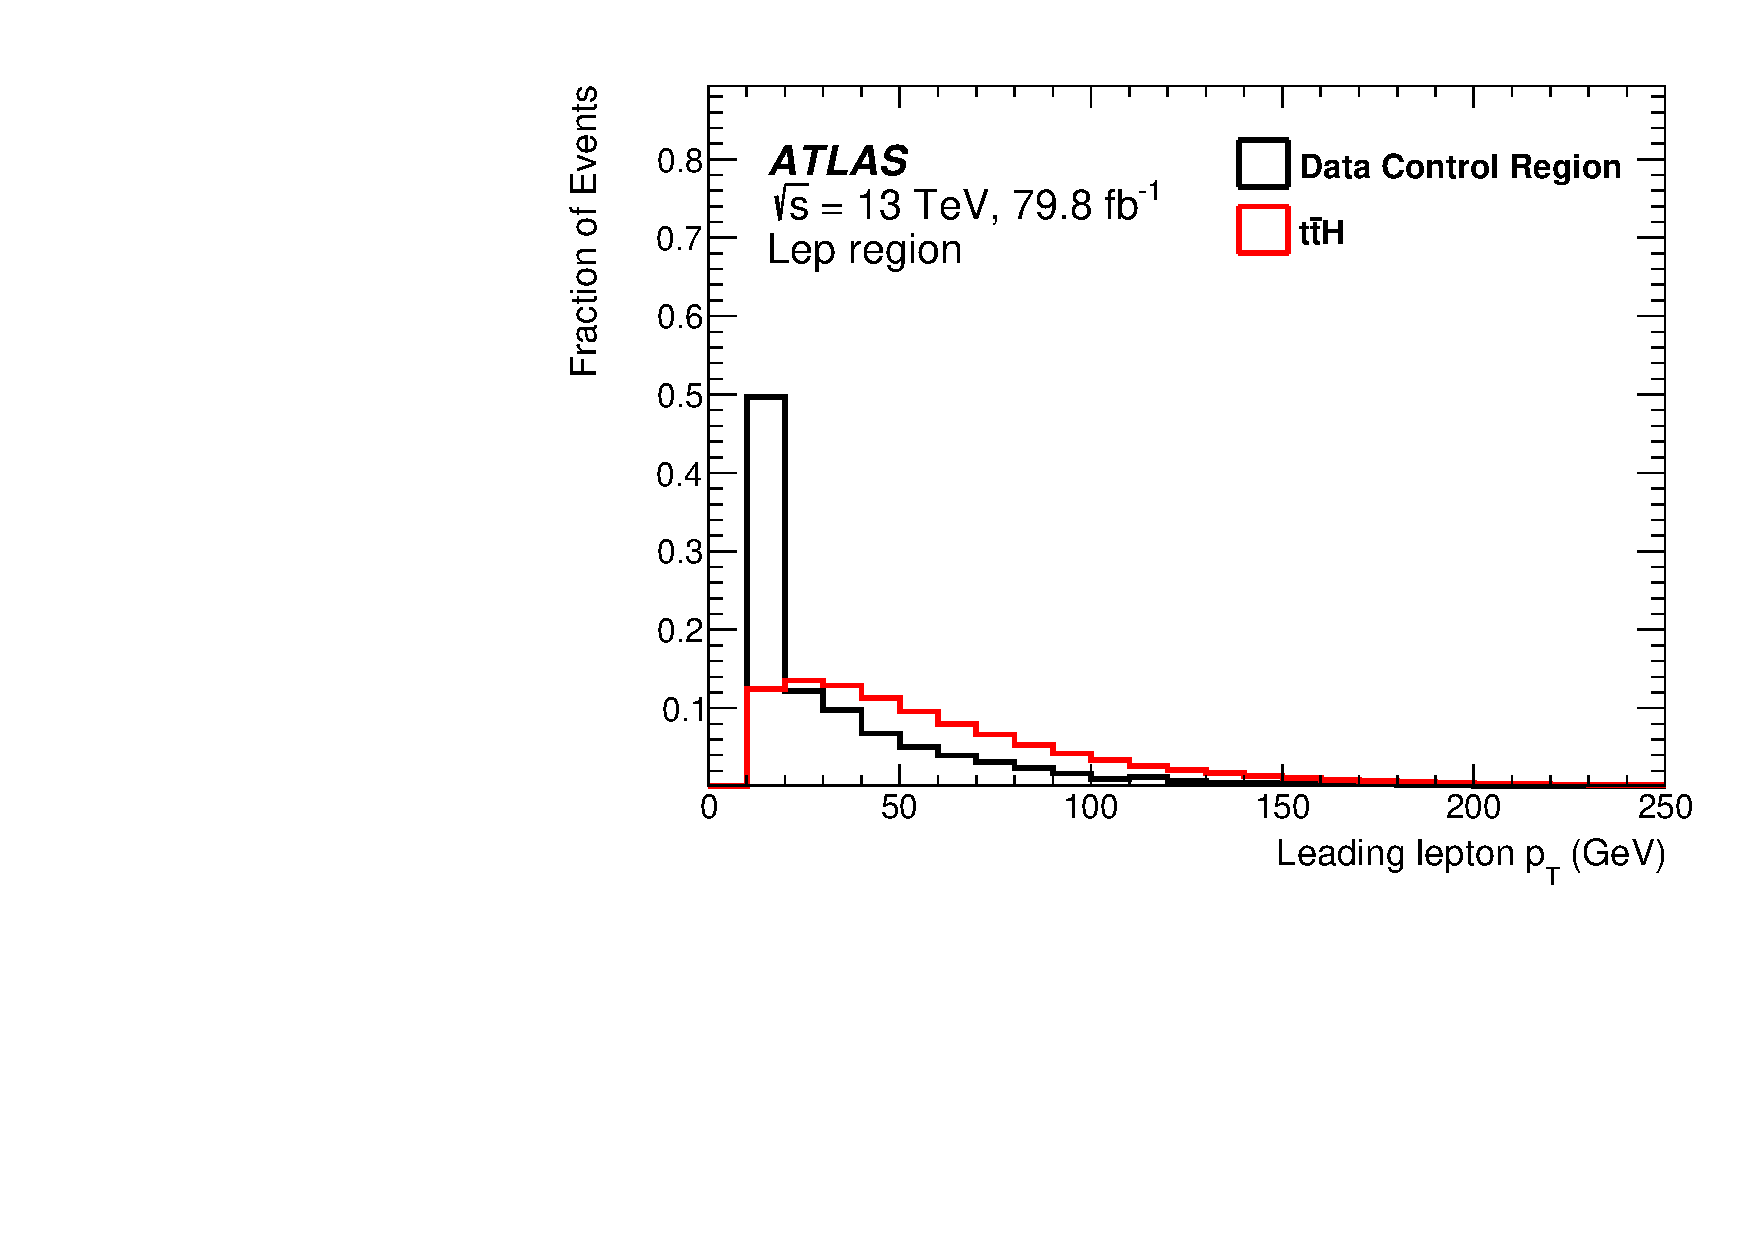
\includegraphics[width=0.31\linewidth]{figures/tthcp_chapter/figaux_11e.pdf}
	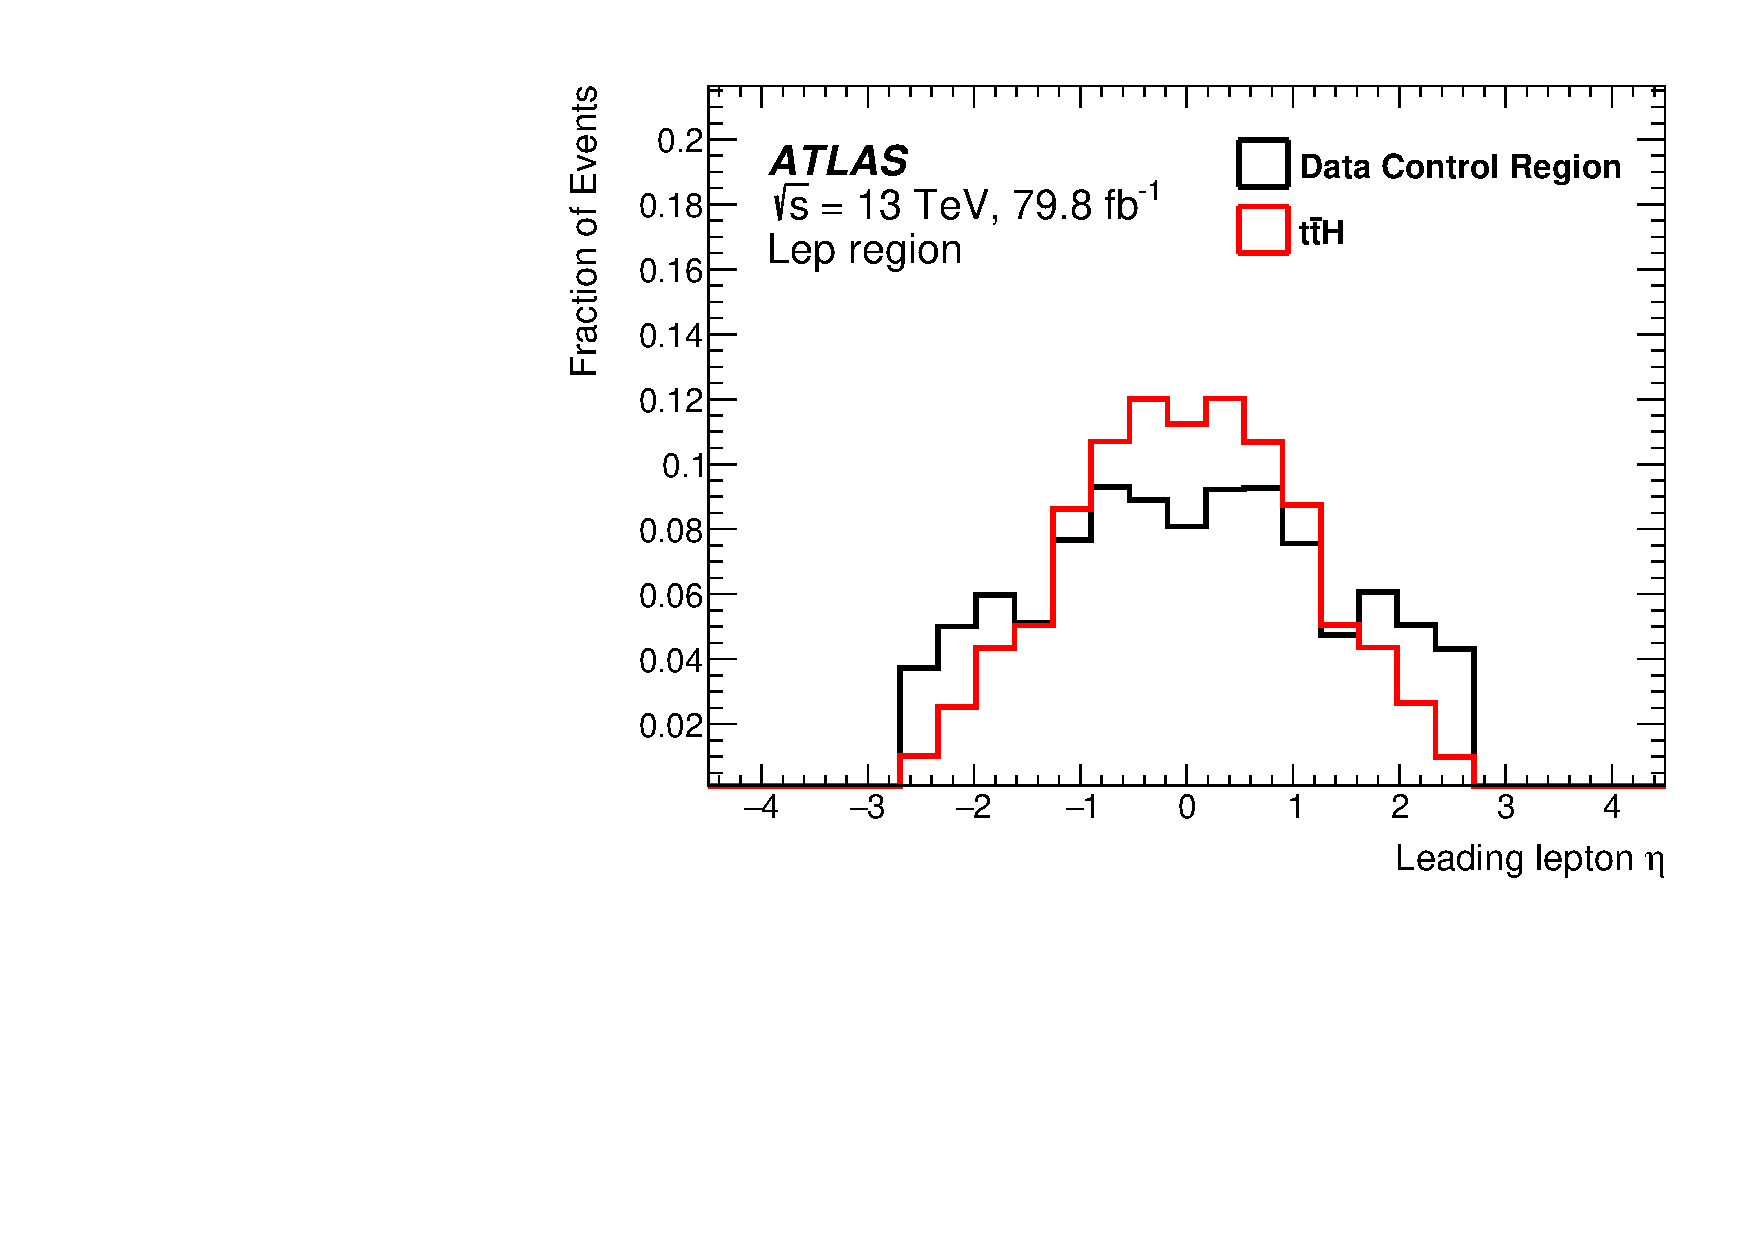
\includegraphics[width=0.31\linewidth]{figures/tthcp_chapter/figaux_11f.pdf}
	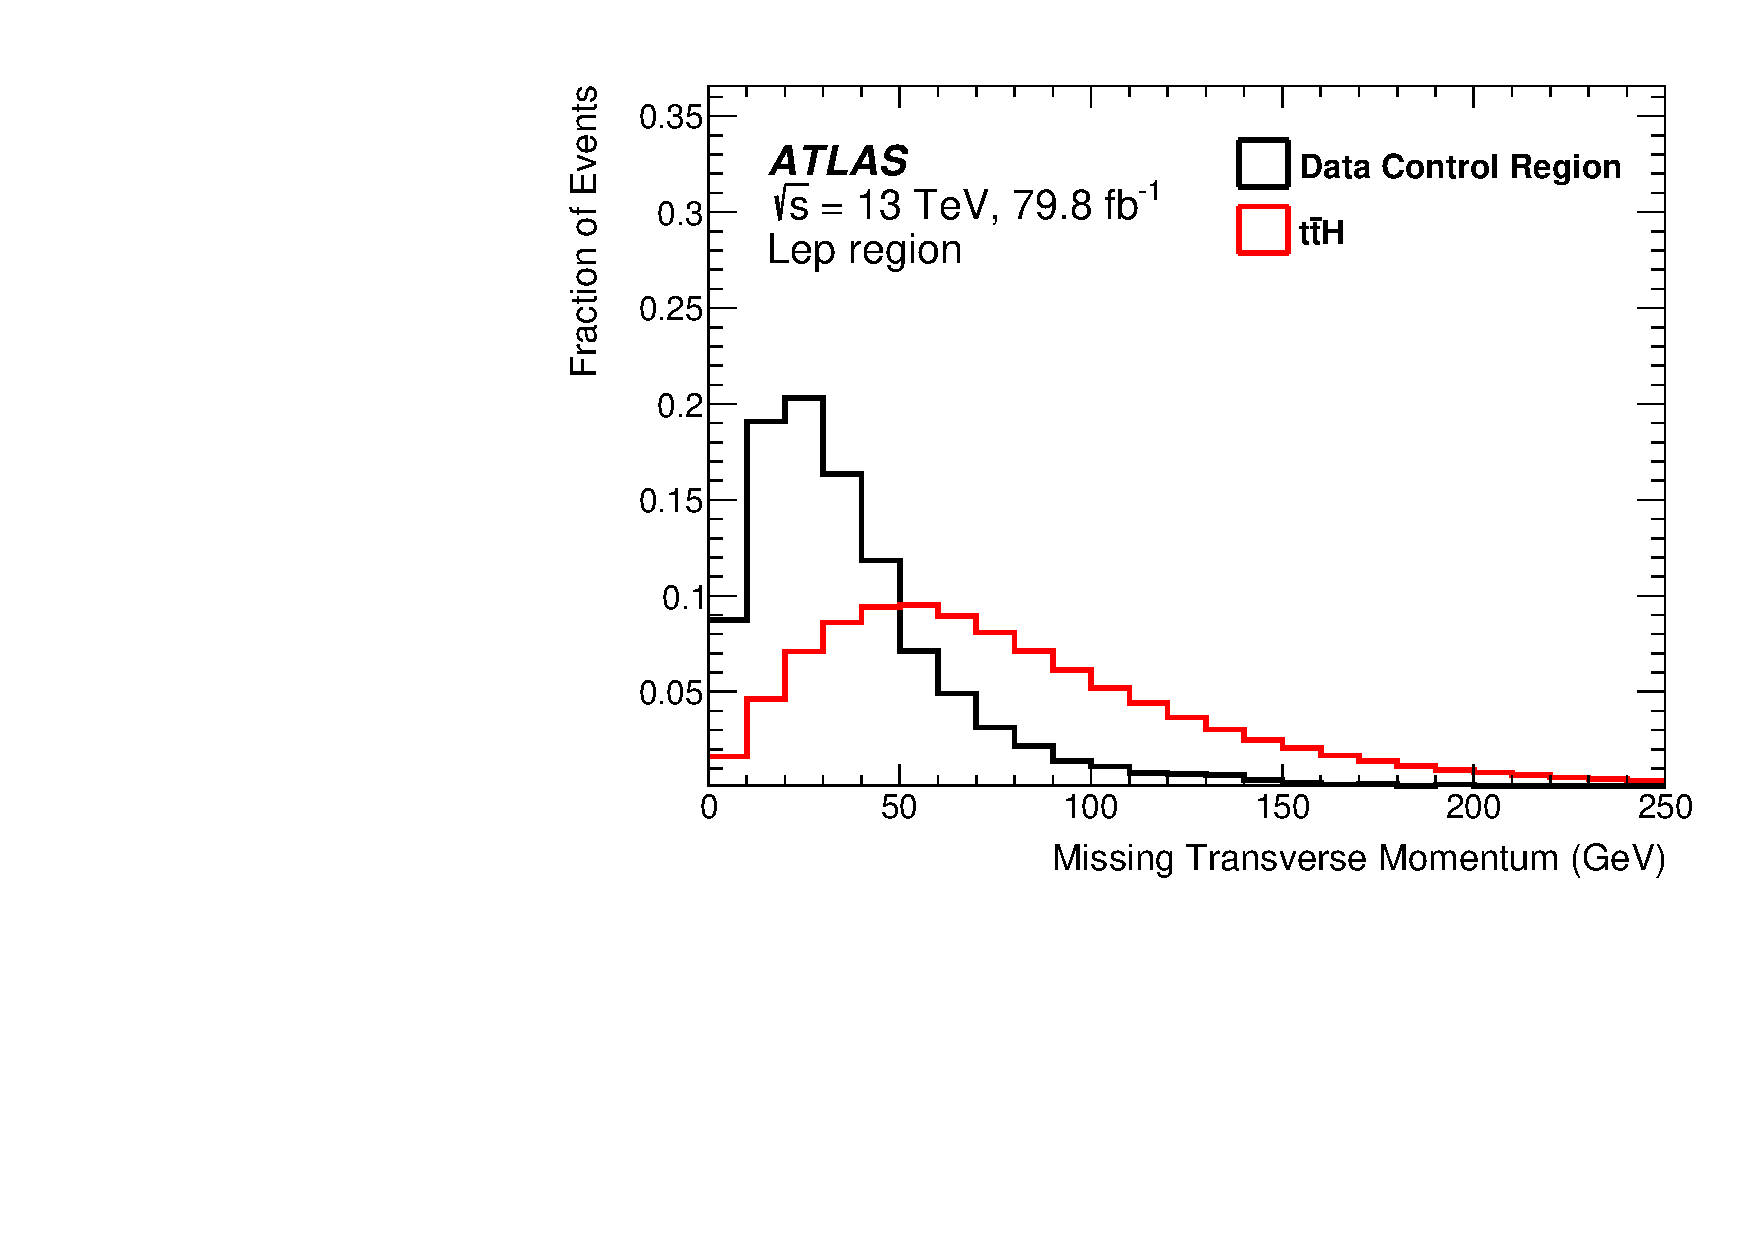
\includegraphics[width=0.31\linewidth]{figures/tthcp_chapter/figaux_11g.pdf}
	\caption{Distributions of training variables for the leptonic background-rejection BDT, trained at $79.8 fb^{-1}$. Taken from \cite{ttH}.}
	\label{fig:SBBDTvarslep}
\end{figure}

\iffalse
\begin{figure}[htbp]
  \centering
        \subfloat[$ttH$ had]{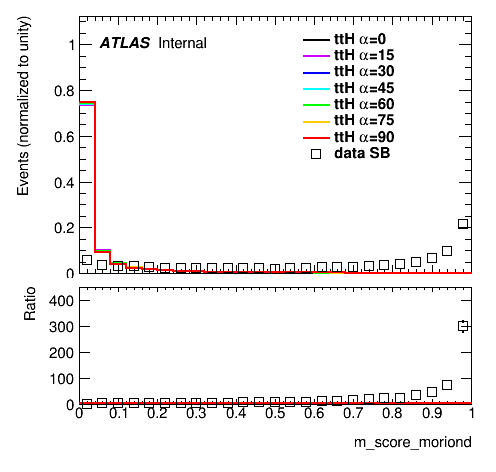
\includegraphics[width=0.3\textwidth]{figures/tthcp_chapter/preselection_and_reconstruction/ttH_had/m_score_wisc.png}}
        \subfloat[$tHjb$ had]{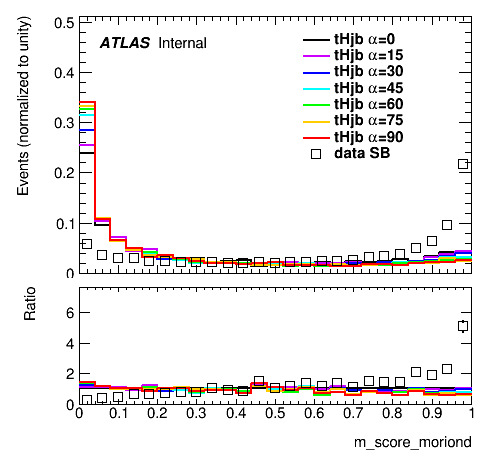
\includegraphics[width=0.3\textwidth]{figures/tthcp_chapter/preselection_and_reconstruction/tHjb_had/m_score_wisc.png}} \\
        \subfloat[$tWH$ had]{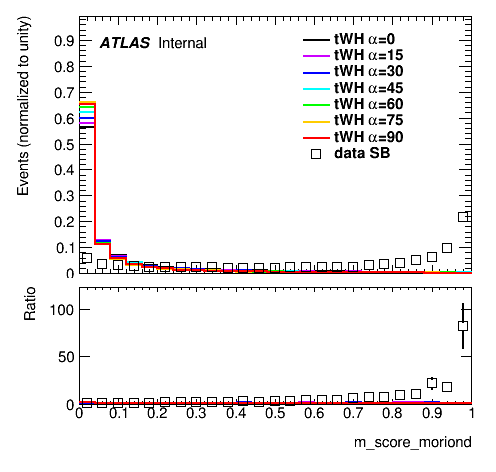
\includegraphics[width=0.3\textwidth]{figures/tthcp_chapter/preselection_and_reconstruction/tWH_had/m_score_wisc.png}}
        \subfloat[$ggF$ had]{\includegraphics[width=0.3\textwidth]{figures/tthp_chapter/preselection_and_reconstruction/ggH_had/m_score_wisc.png}}
  \caption{SB BDT score for $ttH$, $tHjb$, $tWH$ and $ggF$ in the hadronic channel, for various CP mixing scenarios. The open squares show data in the NTI sideband region, which approximates the shape of the continuum background.  }
  \label{fig:moriondhad}
\end{figure}

\begin{figure}[htbp]
  \centering
        \subfloat[$ttH$ lep]{\includegraphics[width=0.3\textwidth]{figures/tthcp_chapter/preselection_and_reconstruction/ttH_lep/m_score_wisc.png}}
        \subfloat[$tHjb$ lep]{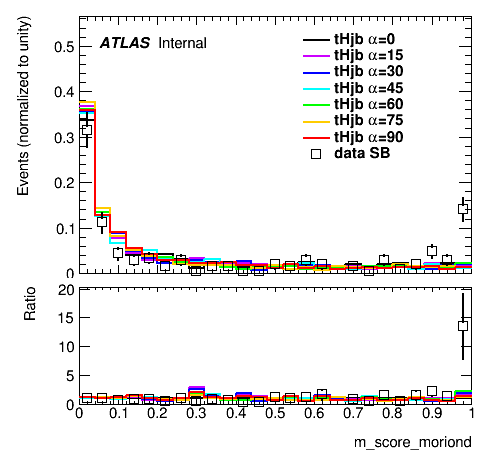
\includegraphics[width=0.3\textwidth]{figures/tthcp_chapter/preselection_and_reconstruction/tHjb_lep/m_score_wisc.png}}
        \subfloat[$tWH$ lep]{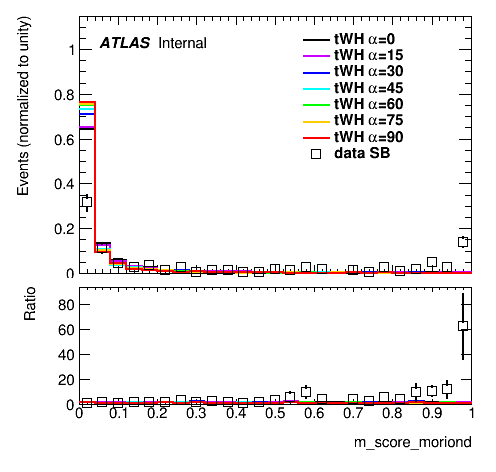
\includegraphics[width=0.3\textwidth]{figures/tthcp_chapter/preselection_and_reconstruction/tWH_lep/m_score_wisc.png}}
  \caption{SB BDT score for $ttH$, $tHjb$ and $tWH$ in the leptonic channel, for various CP mixing scenarios. The open squares show data in the NTI sideband region, which approximates the shape of the continuum background.  }
  \label{fig:moriondlep}
\end{figure}
\fi

\begin{figure}[htbp]
  \centering
        \subfloat[Hadronic]{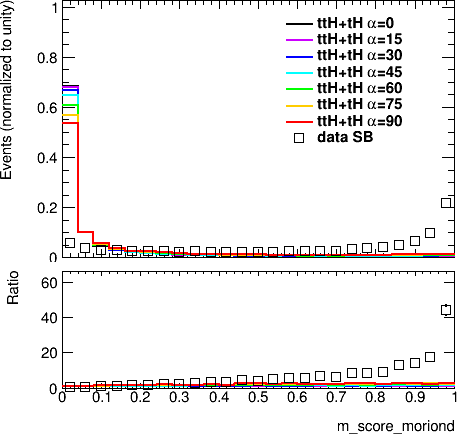
\includegraphics[width=0.4\textwidth]{figures/tthcp_chapter/categorization_xgb/had-vbls/m_score_wisc.png}}
        \subfloat[Leptonic]{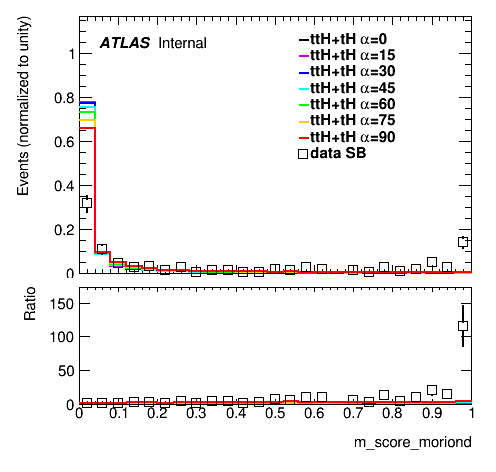
\includegraphics[width=0.4\textwidth]{figures/tthcp_chapter/categorization_xgb/lep-vbls/m_score_wisc.png}}
  \caption{SB BDT score for the sum of $ttH$, $tHjb$ and $tWH$, with relative weights according to their expected cross sections. Shown in (a) for the hadronic channel and (b) for the leptonic channel, for various CP mixing scenarios. The open squares show data in the NTI sideband region, which approximates the shape of the continuum background.  }
  \label{fig:moriondtotal}
\end{figure}


\subsection{CP-Sensitive Observables}

To construct a BDT to discriminate between CP-even and CP-odd $ttH+tH$, a number of variables must be plotted at truth-level in order to determine their dependence on $\alpha$. The HC model $ttH$ and $tH$ samples with alternative values of $\alpha$ generated using MadGraph5\_aMCatNLO are used, added according to their calculated cross-sections given in Table \ref{tab:signal_samples_norm}.

From these plots, it is observed that the strongest variable is the Higgs boson $p_{T}$ : CP-odd $ttH$ and $tH$ have a much more boosted Higgs than CP-even $ttH$ and $tH$, and are more central in $\eta$. Similarly, the angular separation $\Delta \eta$ between the top and anti-top is much larger in CP-odd $ttH$, while the top and anti-top are more back-to-back in azimuthal angle $\Delta \phi$ in CP-even $ttH$ than in CP-odd $ttH$. In $tHjb$ events, it is apparent that the top $p_{T}$ and $\eta$ also have discriminatory power. The mass of the Higgs + leading top system also offers discriminatory power- for $ttH$ and $tWH$ events it increases with $\alpha$, while for $tHjb$ events it decreases with $\alpha$ .

These variables are shown in Figures \ref{fig:ttH_truth} - \ref{fig:tHjb_truth}.


\begin{figure}[!ht] 
  \begin{center}
    \mbox{ 
      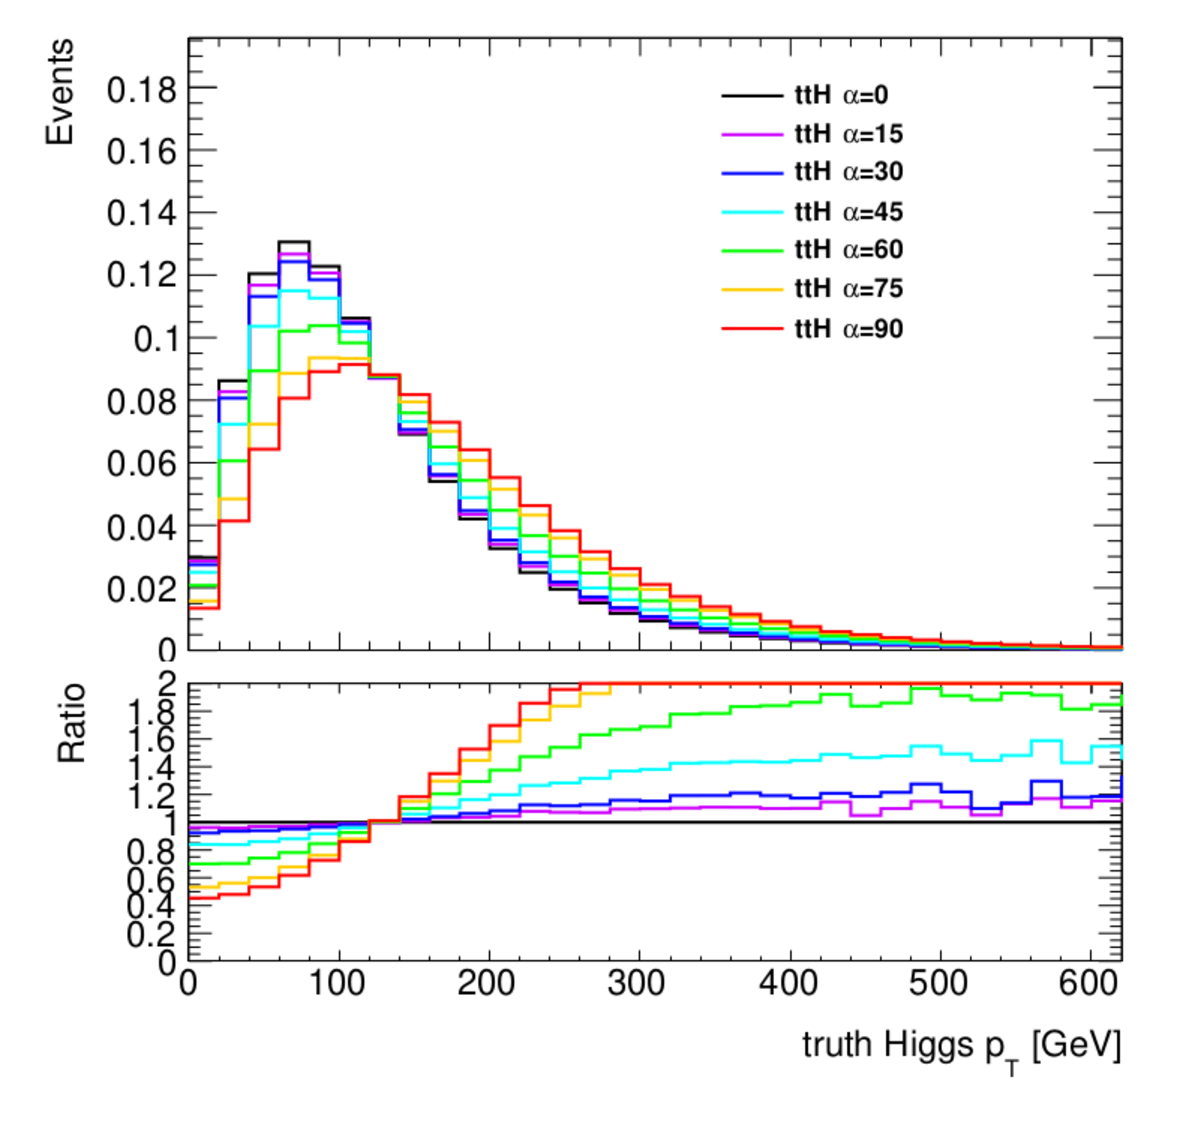
\includegraphics[width=0.31\textwidth]{figures/tthcp_chapter/observables/ttH/c_H_pt.pdf}
      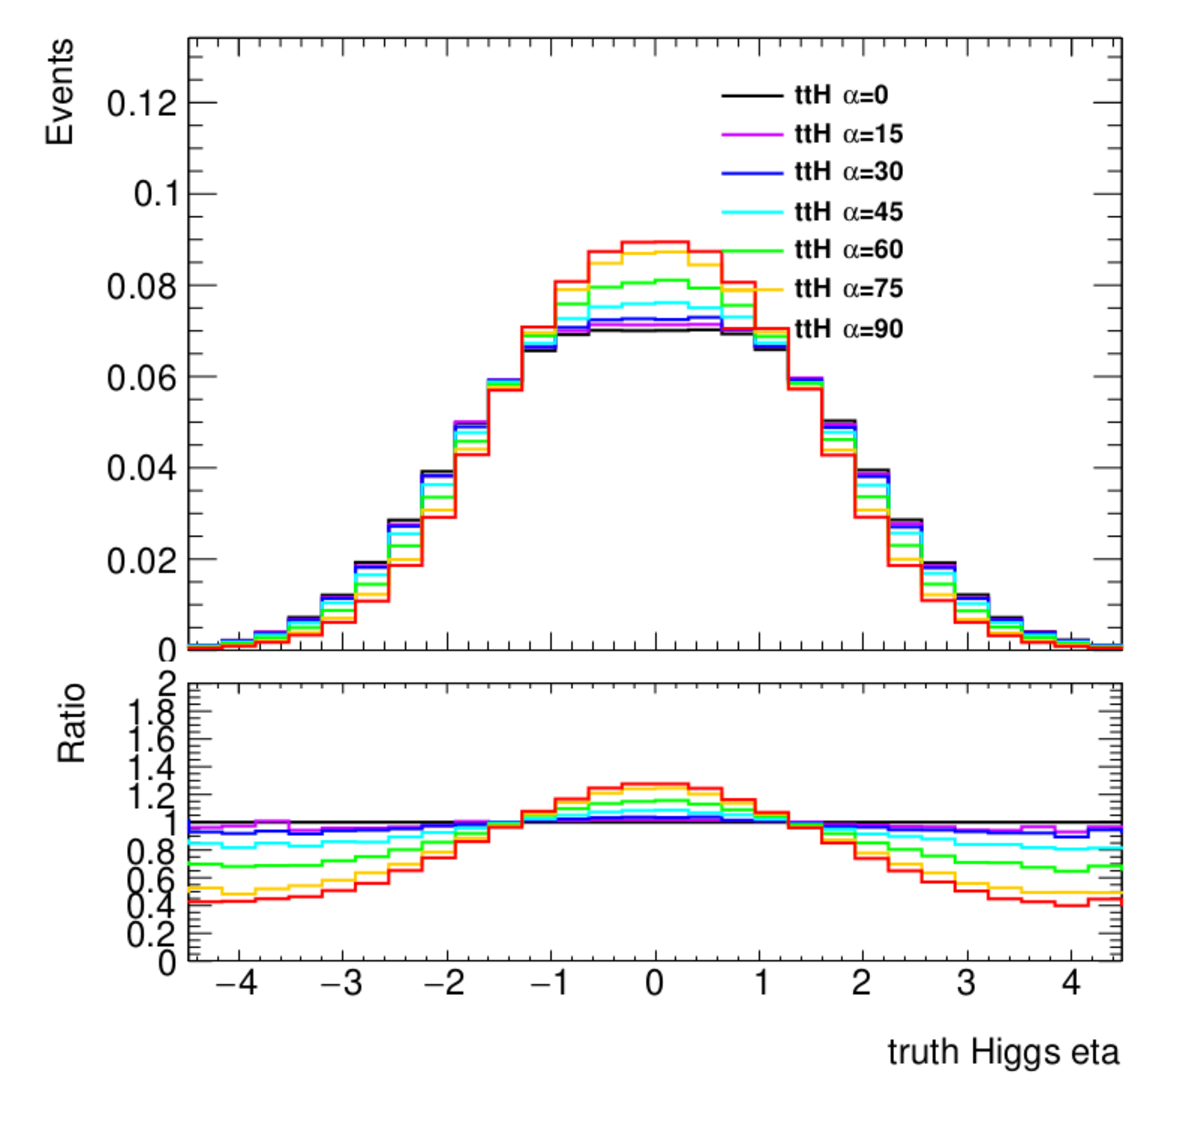
\includegraphics[width=0.31\textwidth]{figures/tthcp_chapter/observables/ttH/c_H_eta.pdf}
      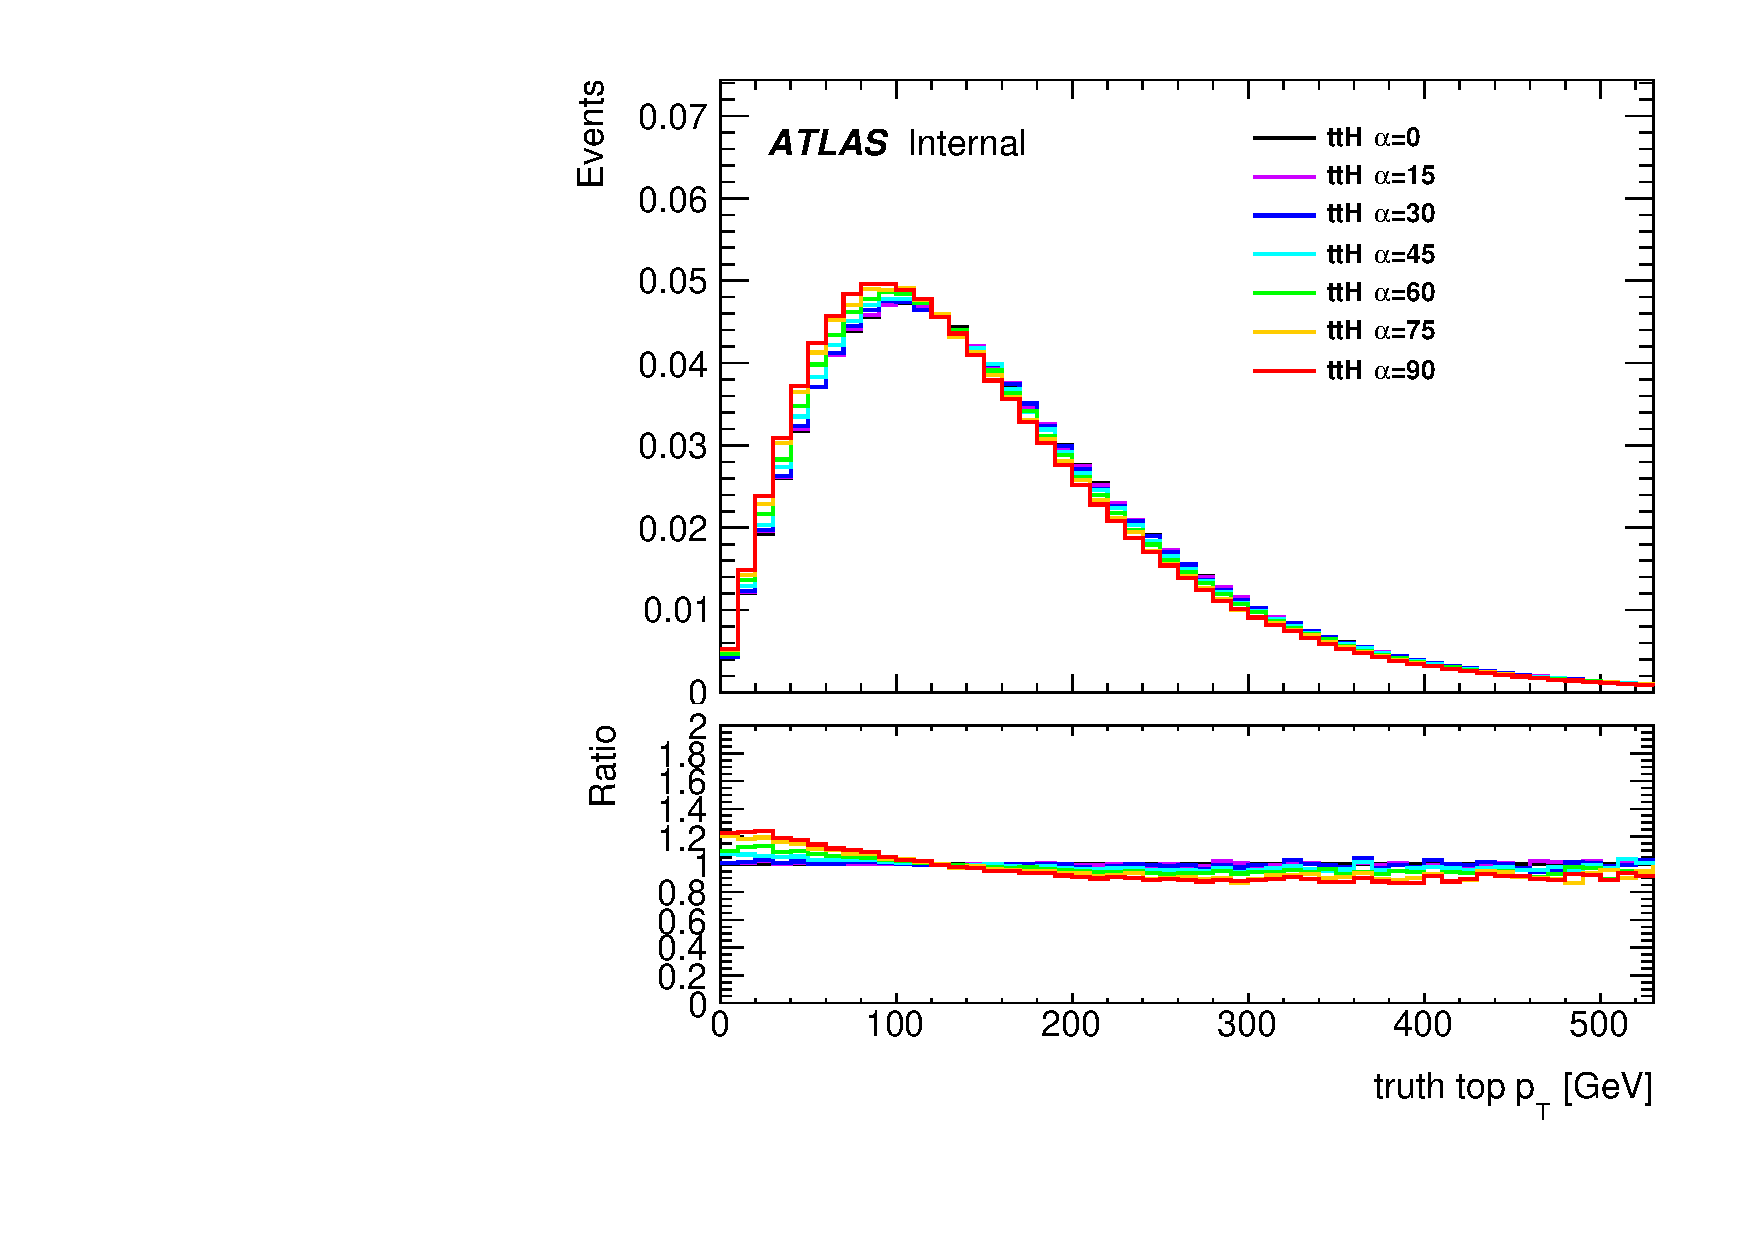
\includegraphics[width=0.31\textwidth]{figures/tthcp_chapter/observables/ttH/c_t_pt.pdf}
    }
    \mbox{ 
      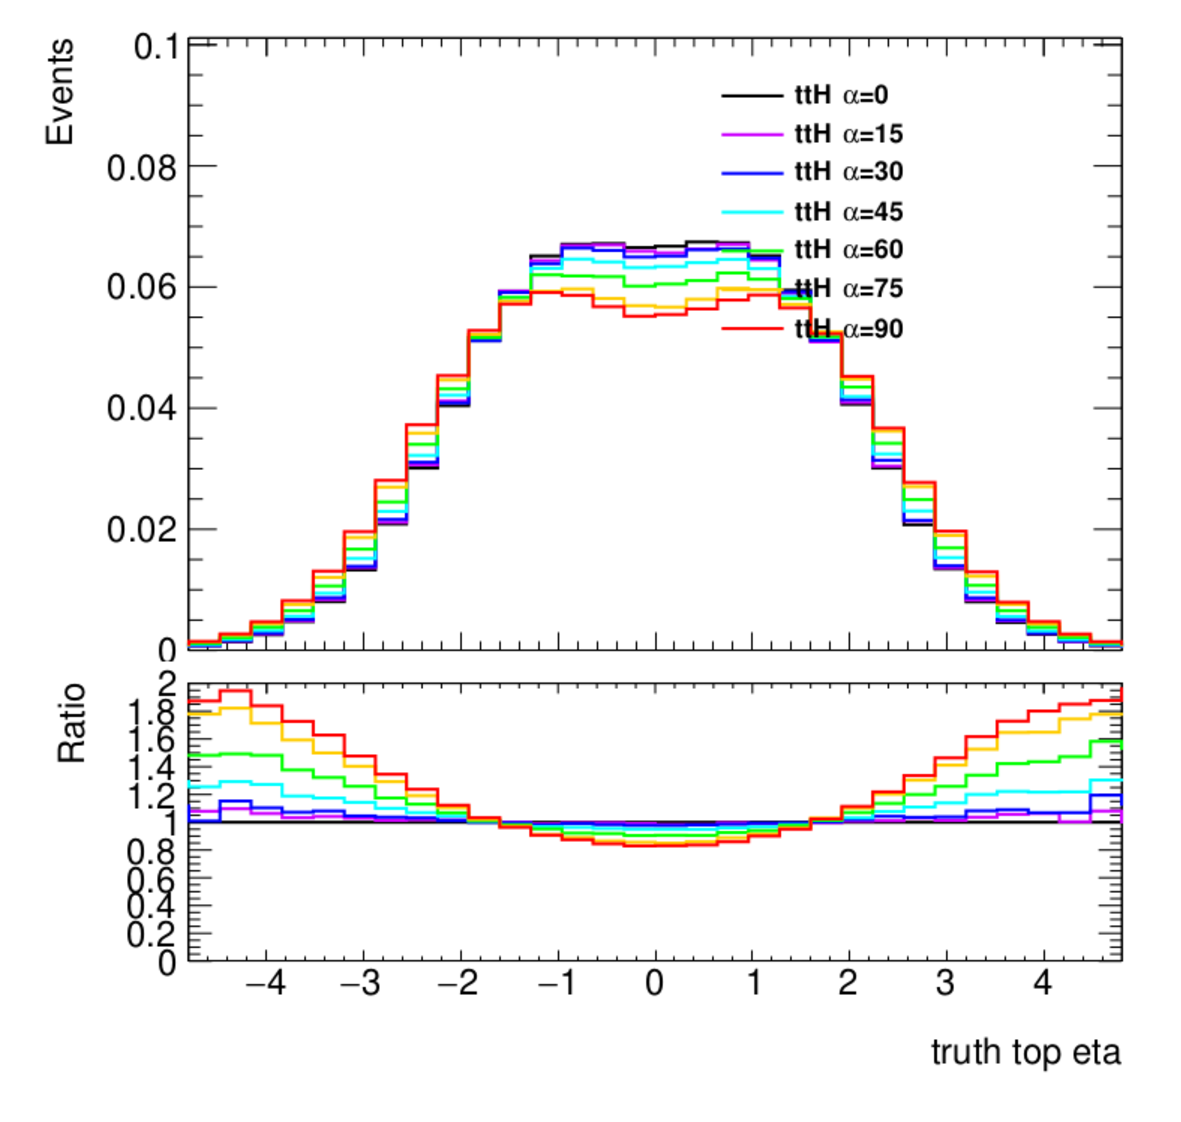
\includegraphics[width=0.31\textwidth]{figures/tthcp_chapter/observables/ttH/c_t_eta.pdf}
      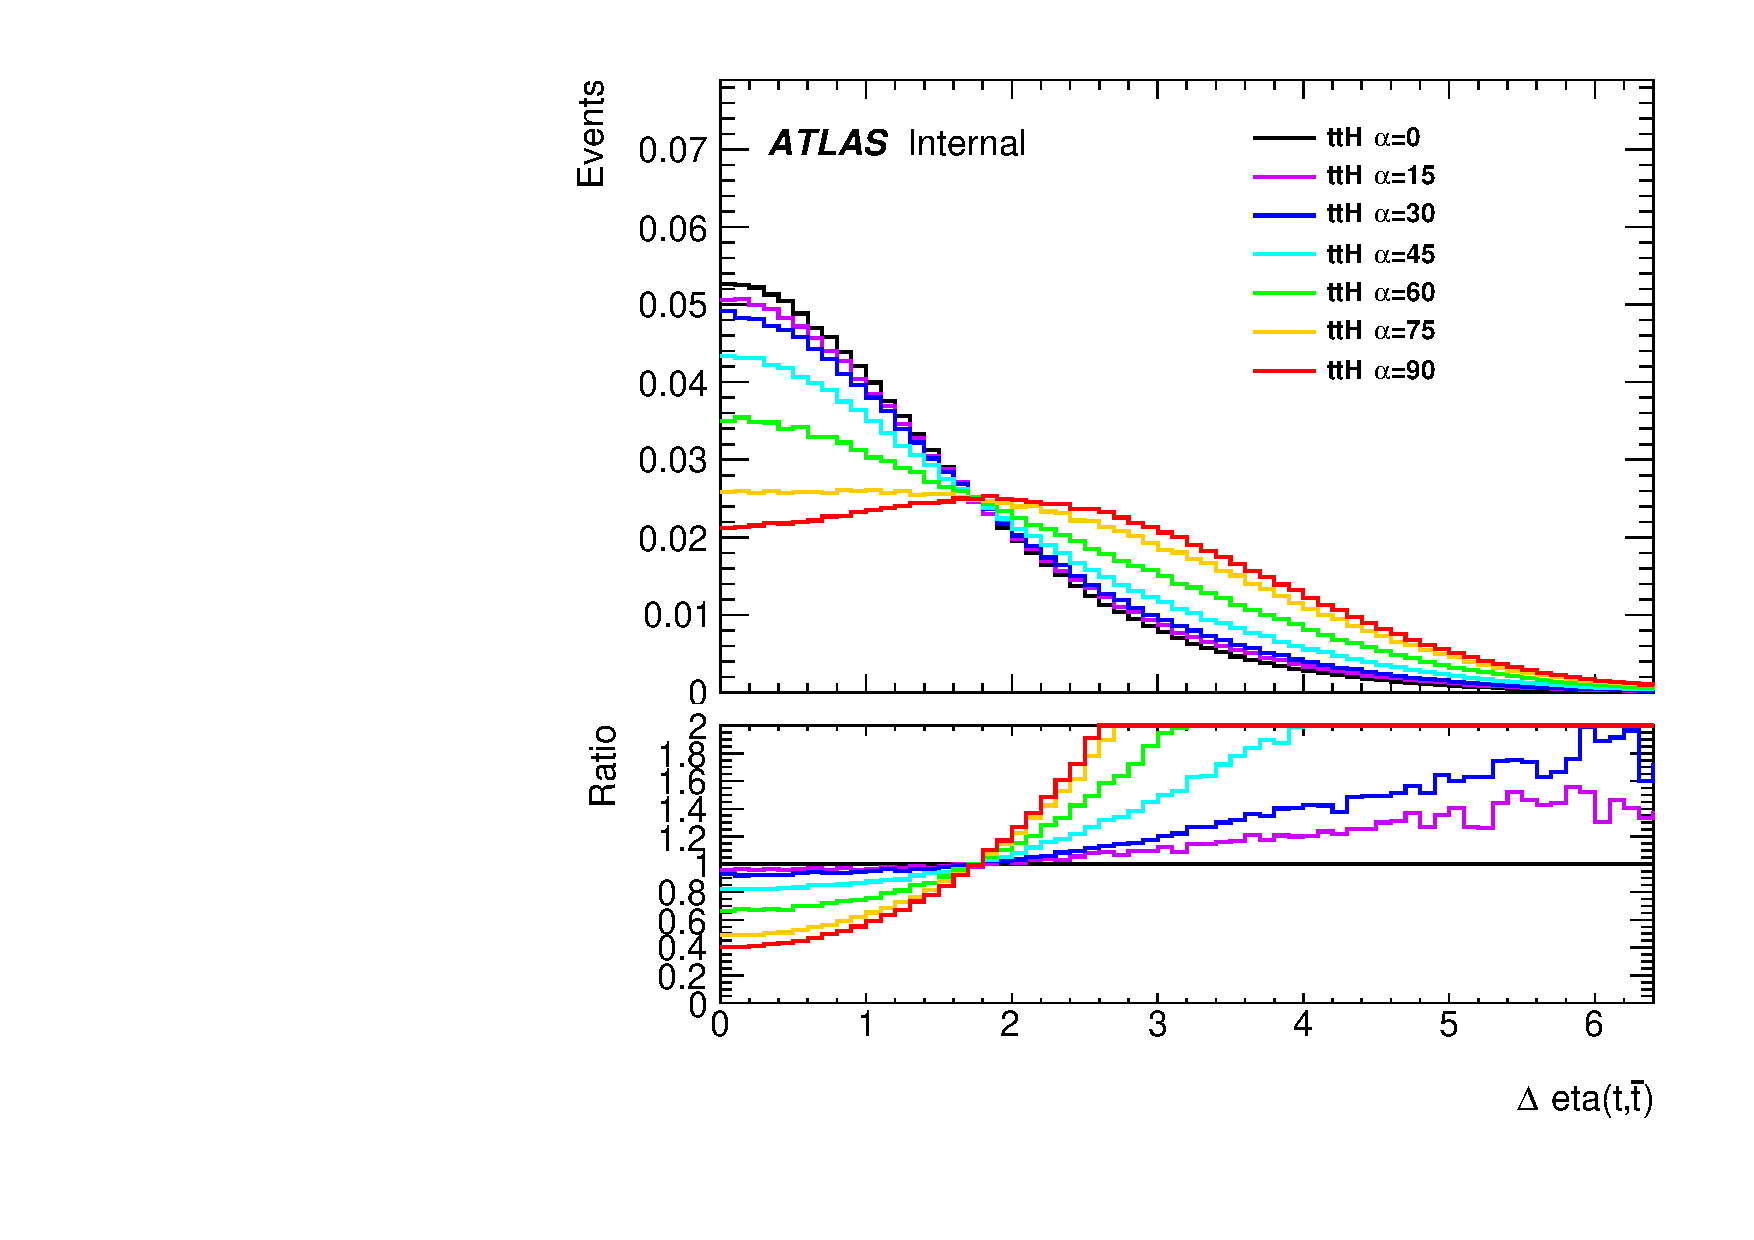
\includegraphics[width=0.31\textwidth]{figures/tthcp_chapter/observables/ttH/c_delta_eta_tt.pdf}
      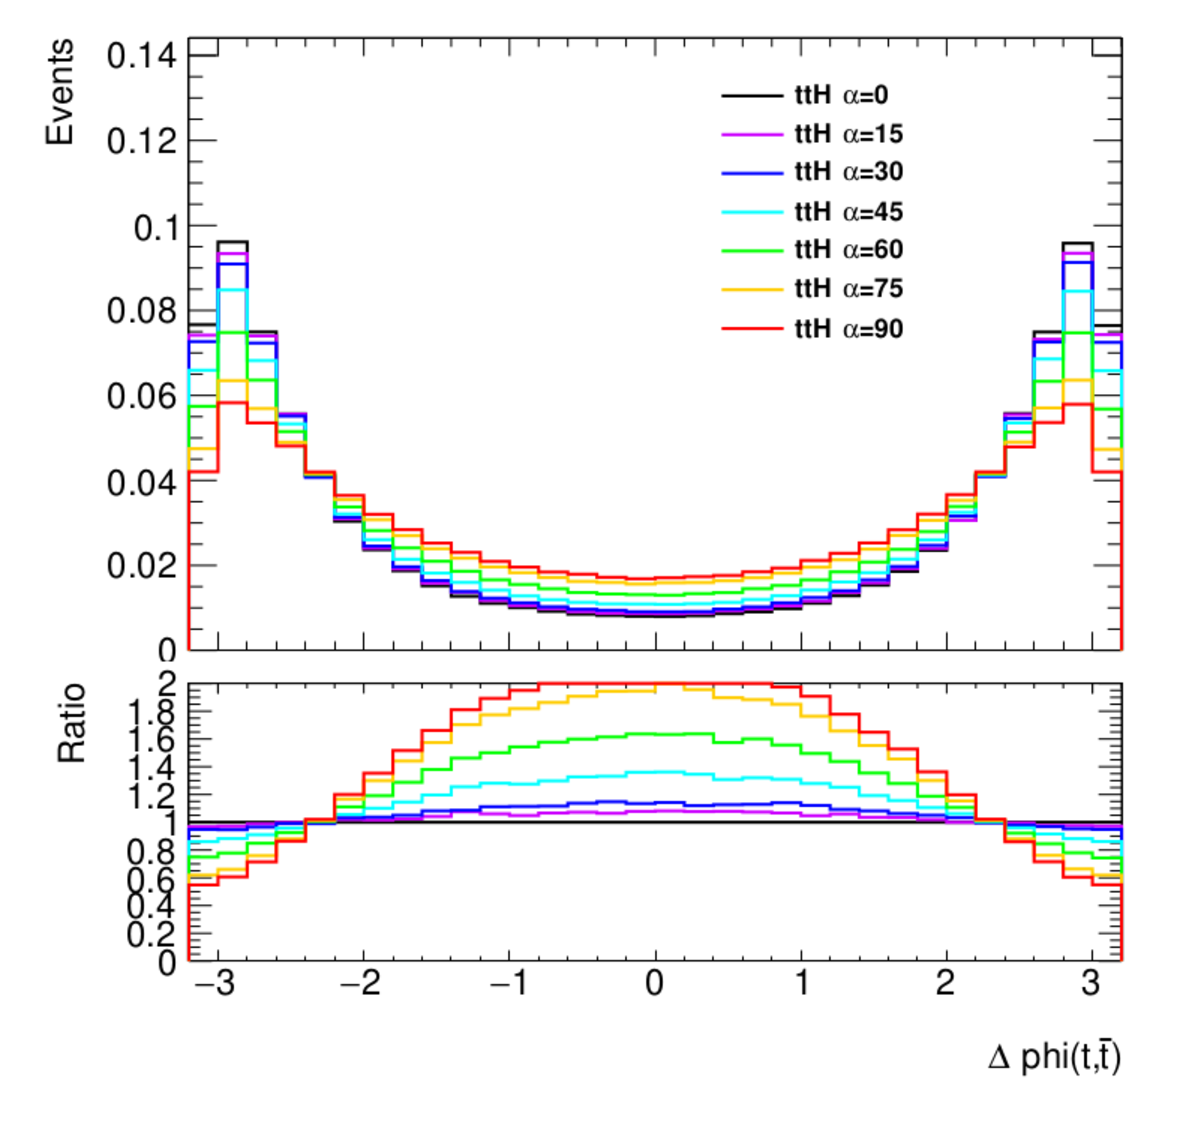
\includegraphics[width=0.31\textwidth]{figures/tthcp_chapter/observables/ttH/c_delta_phi_tt.pdf}
    }
    \mbox{ 
    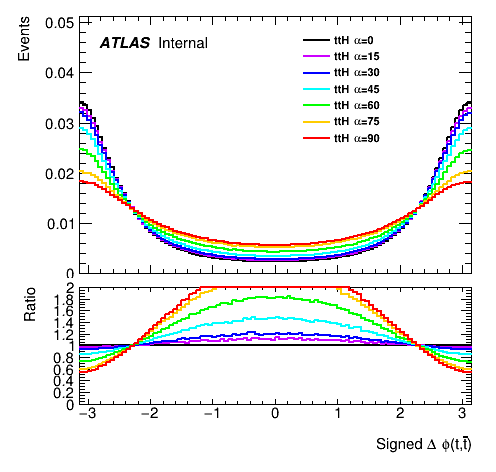
\includegraphics[width=0.31\textwidth]{figures/tthcp_chapter/observables/ttH/c_delta_phi_tt_signed.png}
	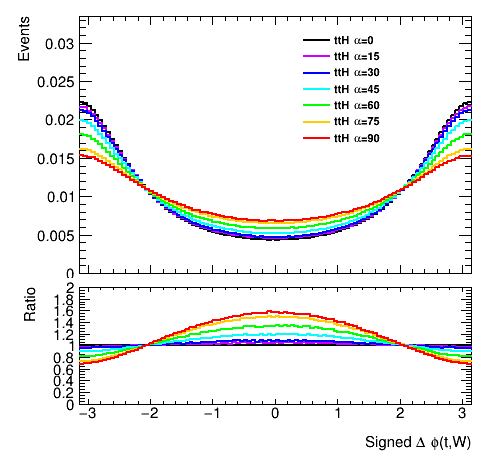
\includegraphics[width=0.31\textwidth]{figures/tthcp_chapter/observables/ttH/c_delta_phi_tW_signed.png} 
	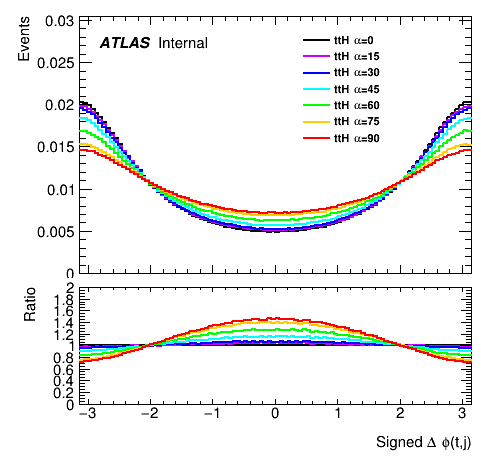
\includegraphics[width=0.31\textwidth]{figures/tthcp_chapter/observables/ttH/c_delta_phi_tj_signed.png} 
	}
	\mbox{ 
      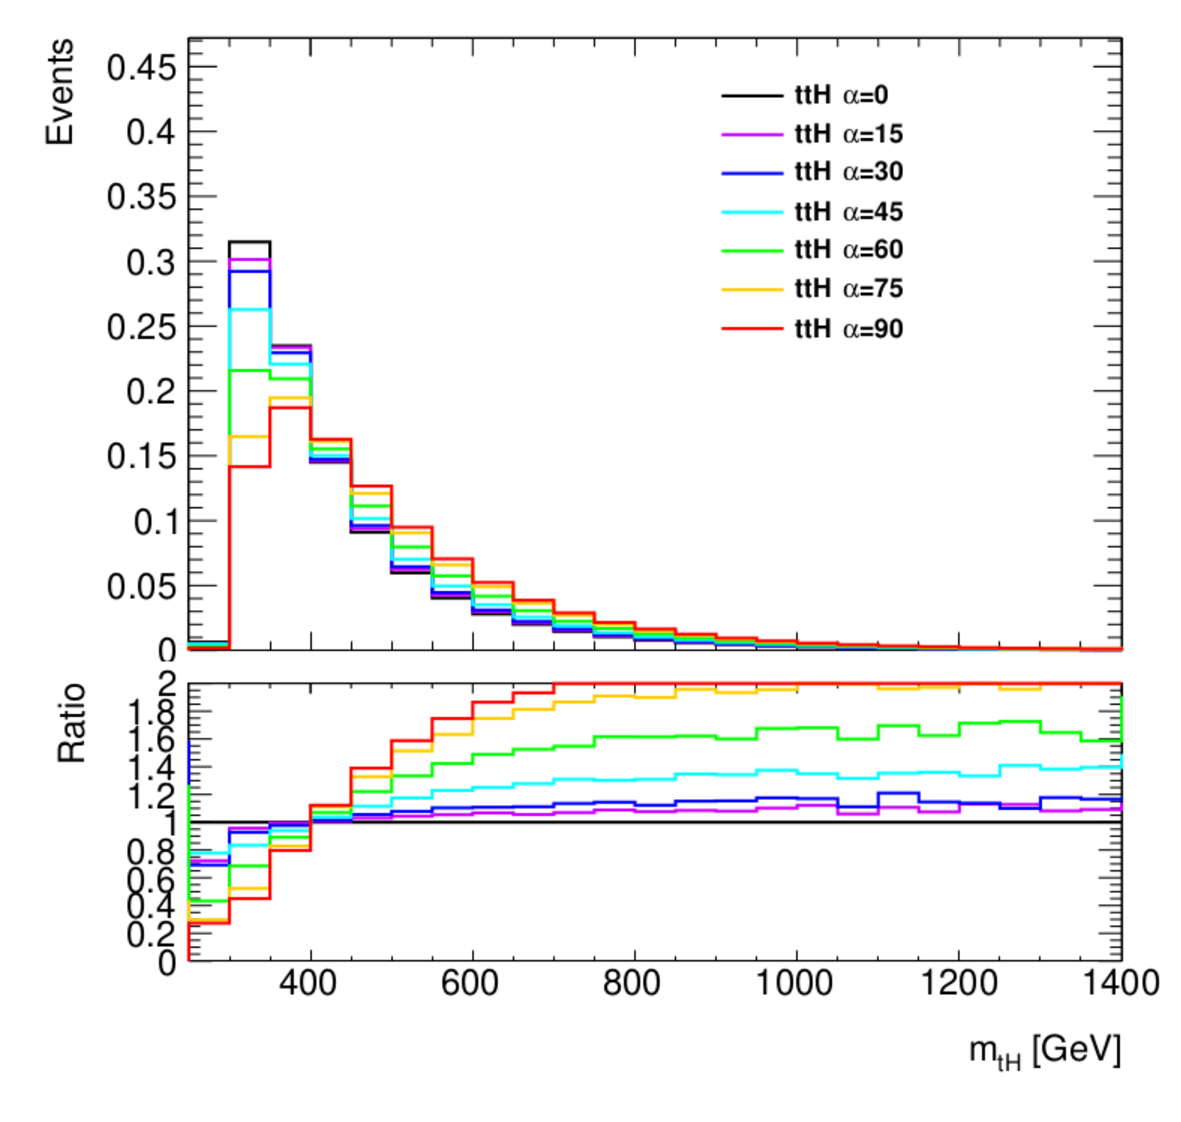
\includegraphics[width=0.31\textwidth]{figures/tthcp_chapter/observables/ttH/c_tH_m.pdf}
    }
  \end{center}
  \caption{Truth-level distributions in $t\bar{t}H$ Monte Carlo of the Higgs boson $p_{T}$, Higgs boson $\eta$, and top quark $p_{T}$ (top row), top quark $\eta$ and angular separation between top and anti-top quarks (second row), signed $\Delta\phi$ between (a) the two top quarks, (b) a top quark and the daughter W of the other top quark, and (c) a top quark and the highest $p_{T}$ light jet from the hadronic decay of the other top's daughter W (third row) and invariant mass of the top-Higgs system (bottom row) for different values of the CP mixing angle $\alpha$.}
  \label{fig:ttH_truth}
\end{figure}


\begin{figure}[!ht] 
  \begin{center}
    \mbox{ 
      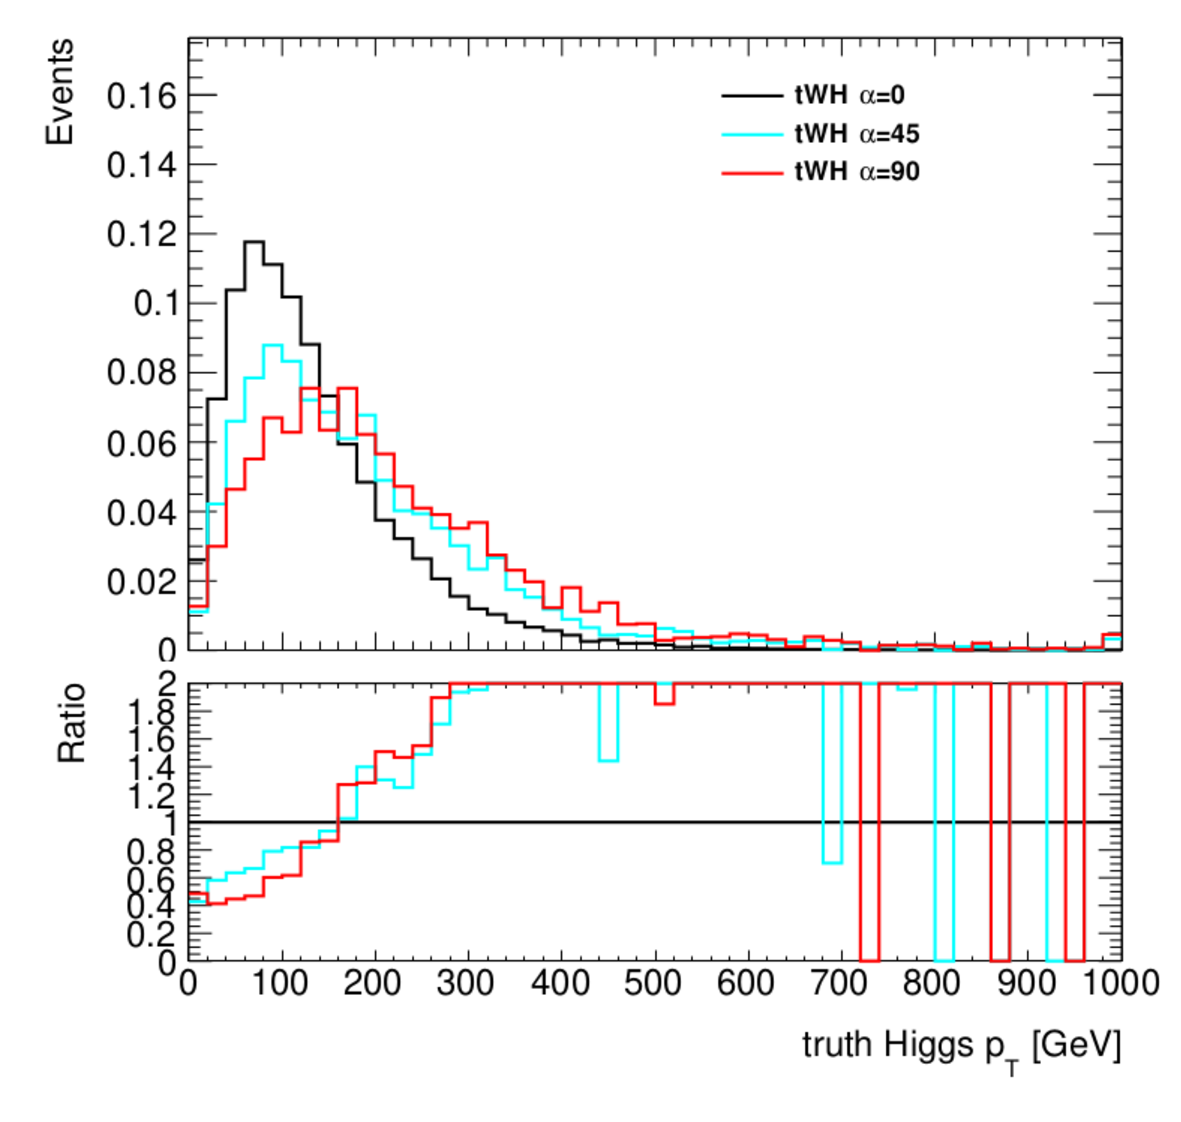
\includegraphics[width=0.35\textwidth]{figures/tthcp_chapter/observables/tWH/c_H_pt.pdf}
      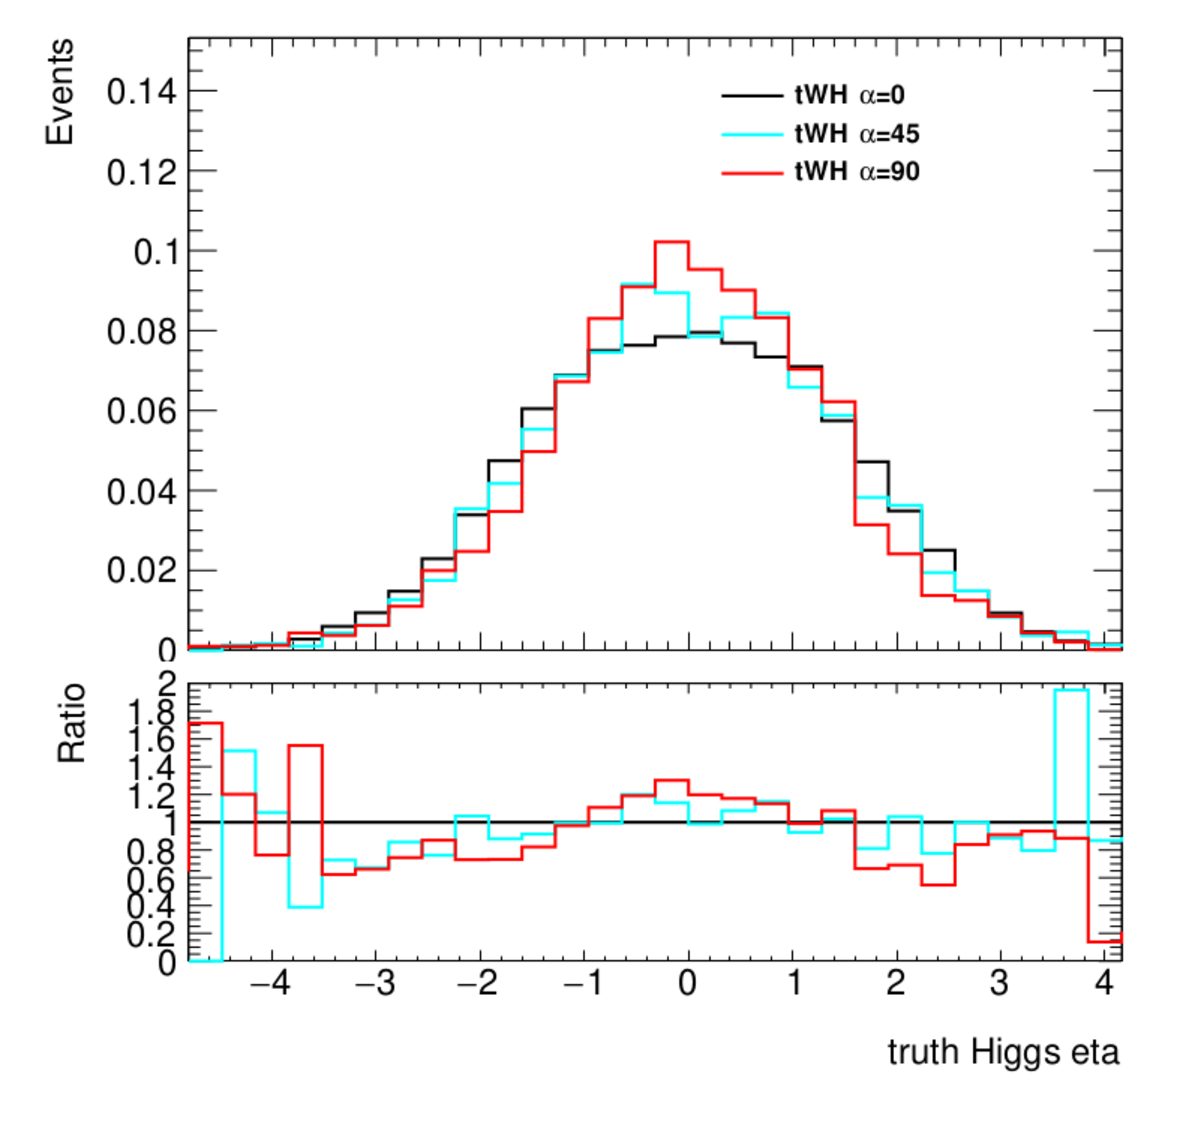
\includegraphics[width=0.35\textwidth]{figures/tthcp_chapter/observables/tWH/c_H_eta.pdf}
    }
    \mbox{ 
      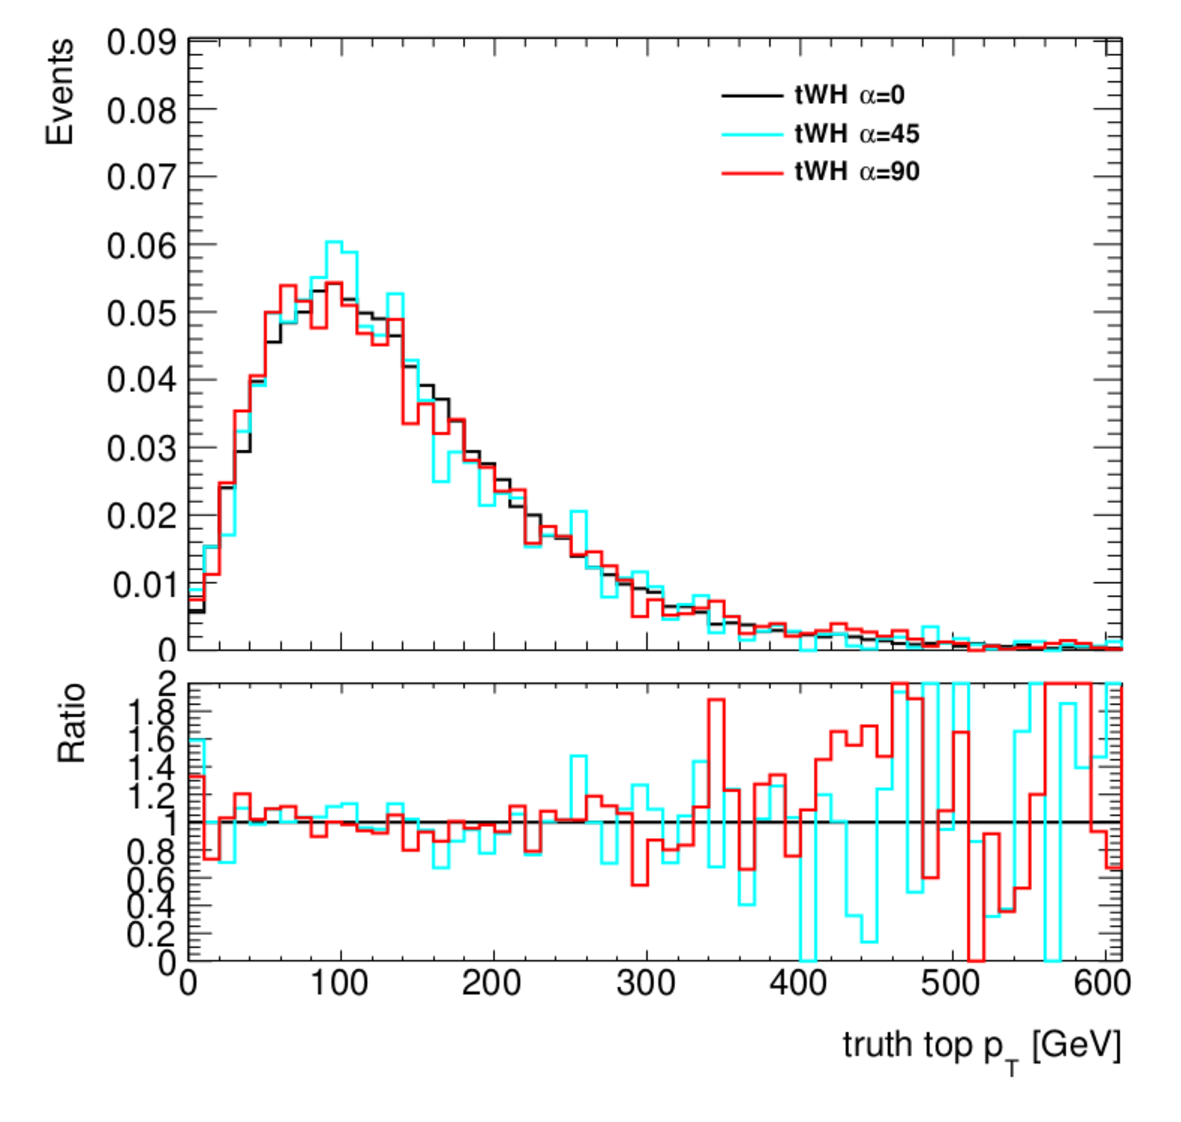
\includegraphics[width=0.35\textwidth]{figures/tthcp_chapter/observables/tWH/c_t_pt.pdf}
      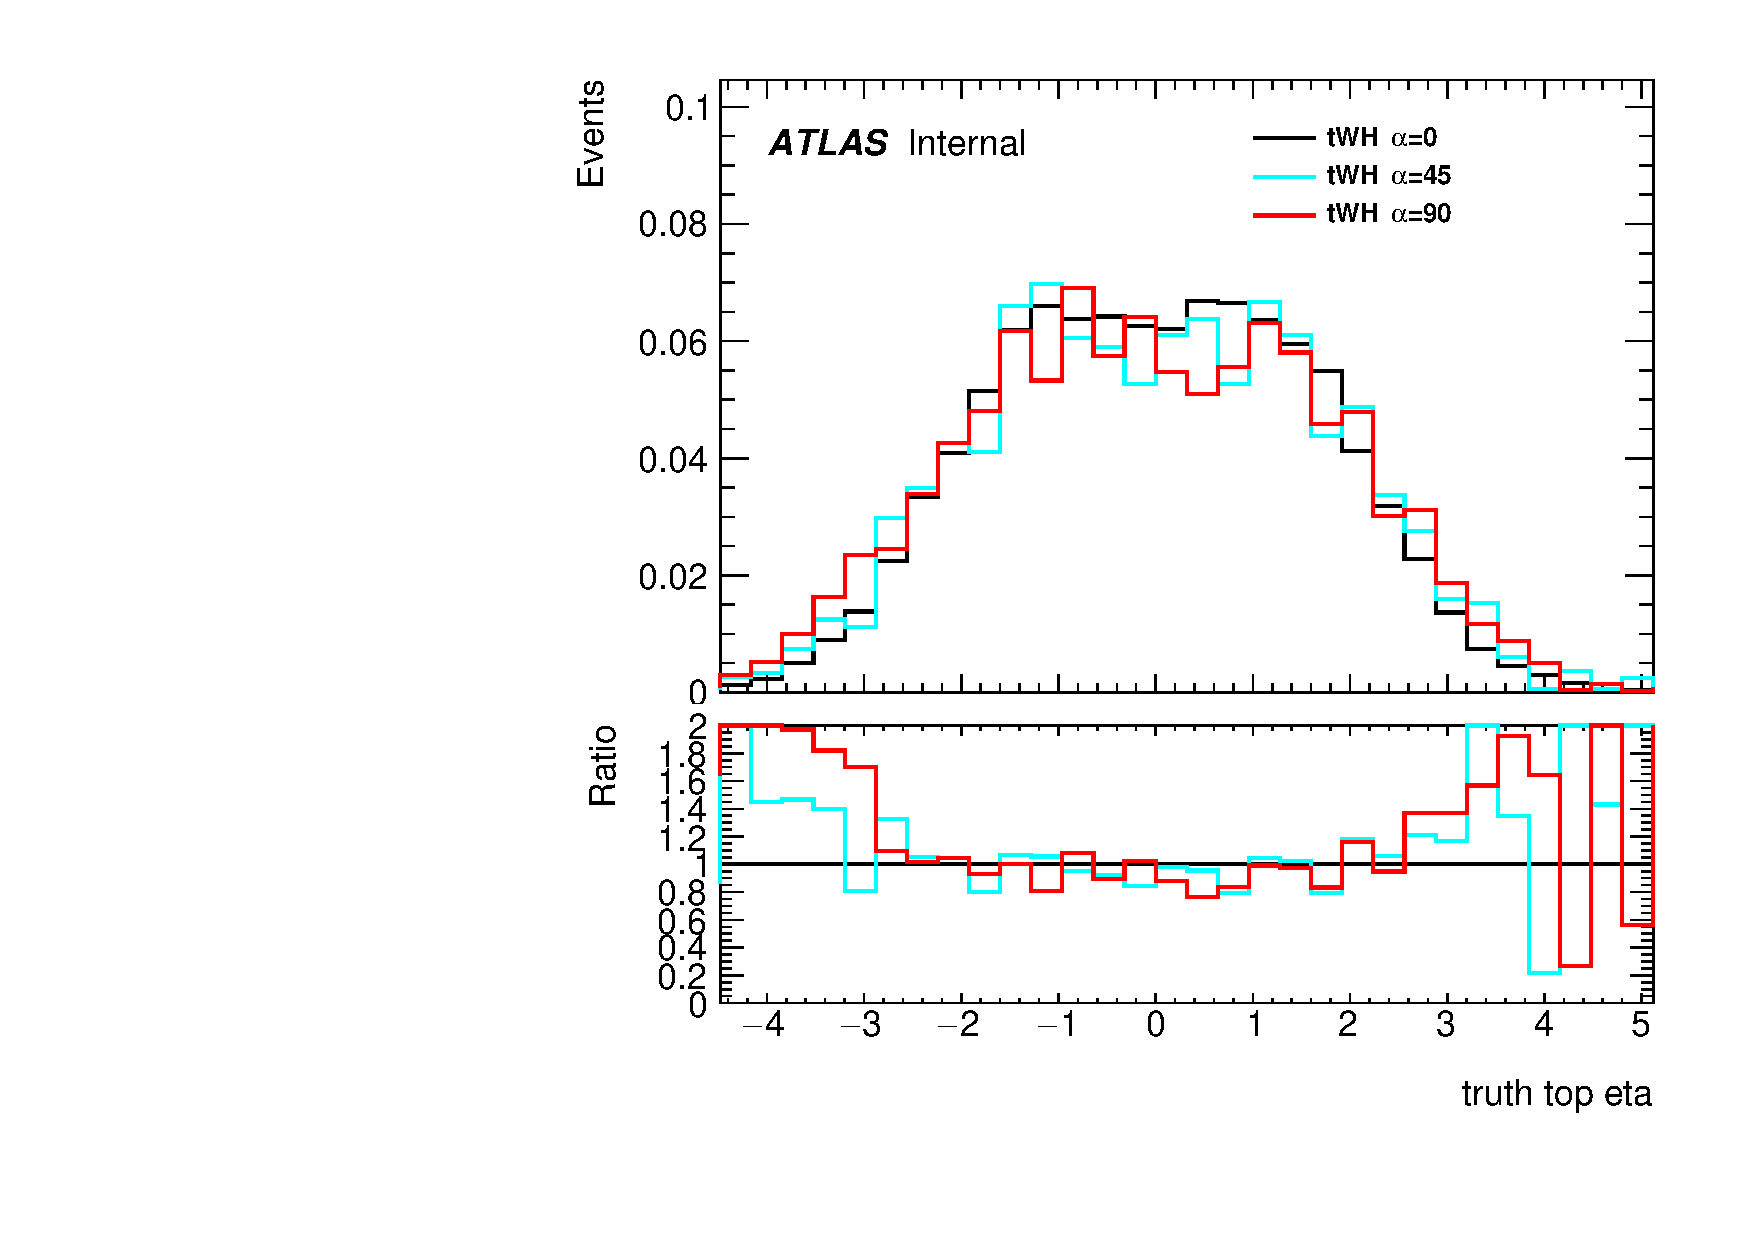
\includegraphics[width=0.35\textwidth]{figures/tthcp_chapter/observables/tWH/c_t_eta.pdf}
    }
    \mbox{ 
      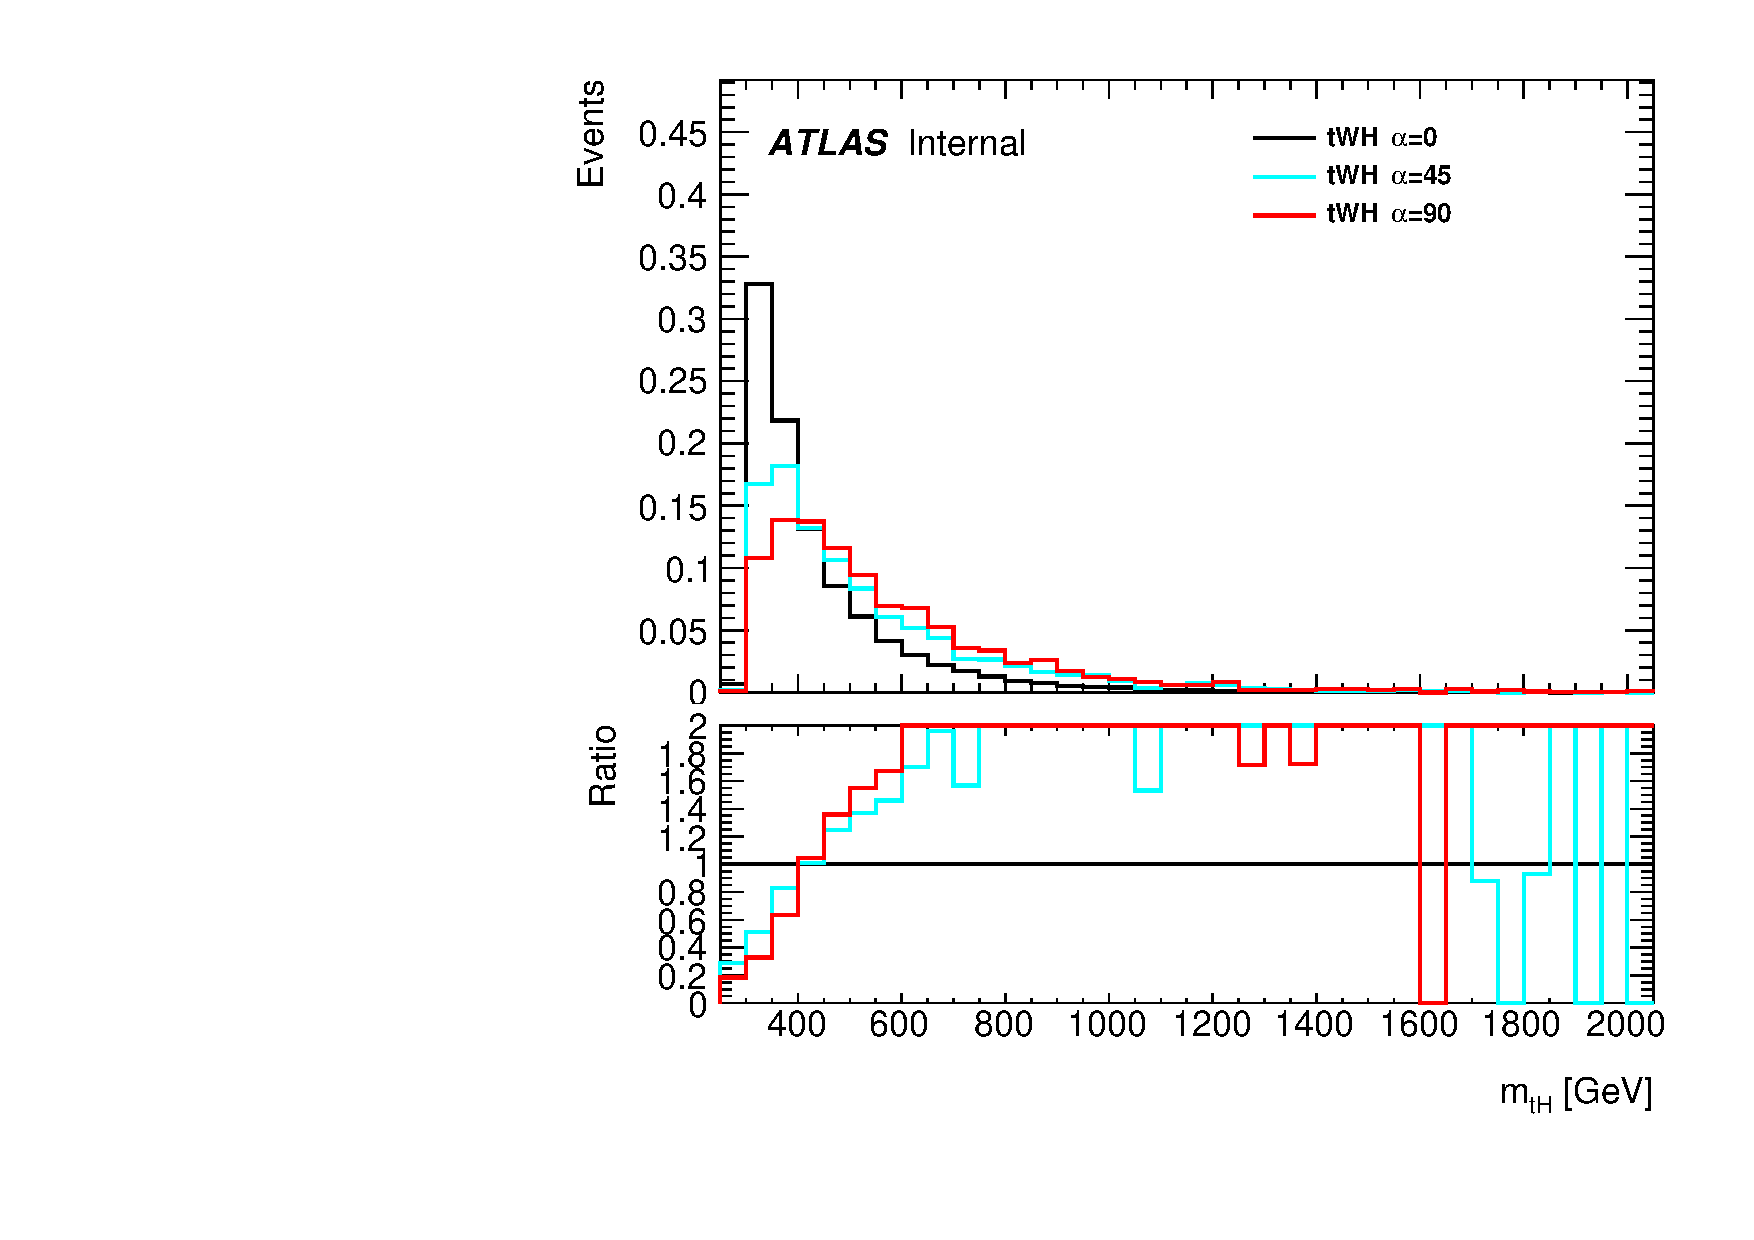
\includegraphics[width=0.35\textwidth]{figures/tthcp_chapter/observables/tWH/c_tH_m.pdf}
    }
  \end{center}
  \caption{Truth-level distributions in $tWH$ Monte Carlo of the Higgs boson $p_{T}$ and $\eta$ (top), top quark $p_{T}$ and $\eta$ (middle) and invariant mass of the top-Higgs system (bottom) for different values of the CP mixing angle $\alpha$.}
  \label{fig:tWH_truth}
\end{figure}
\clearpage


\begin{figure}[!ht] 
  \begin{center}
    \mbox{ 
      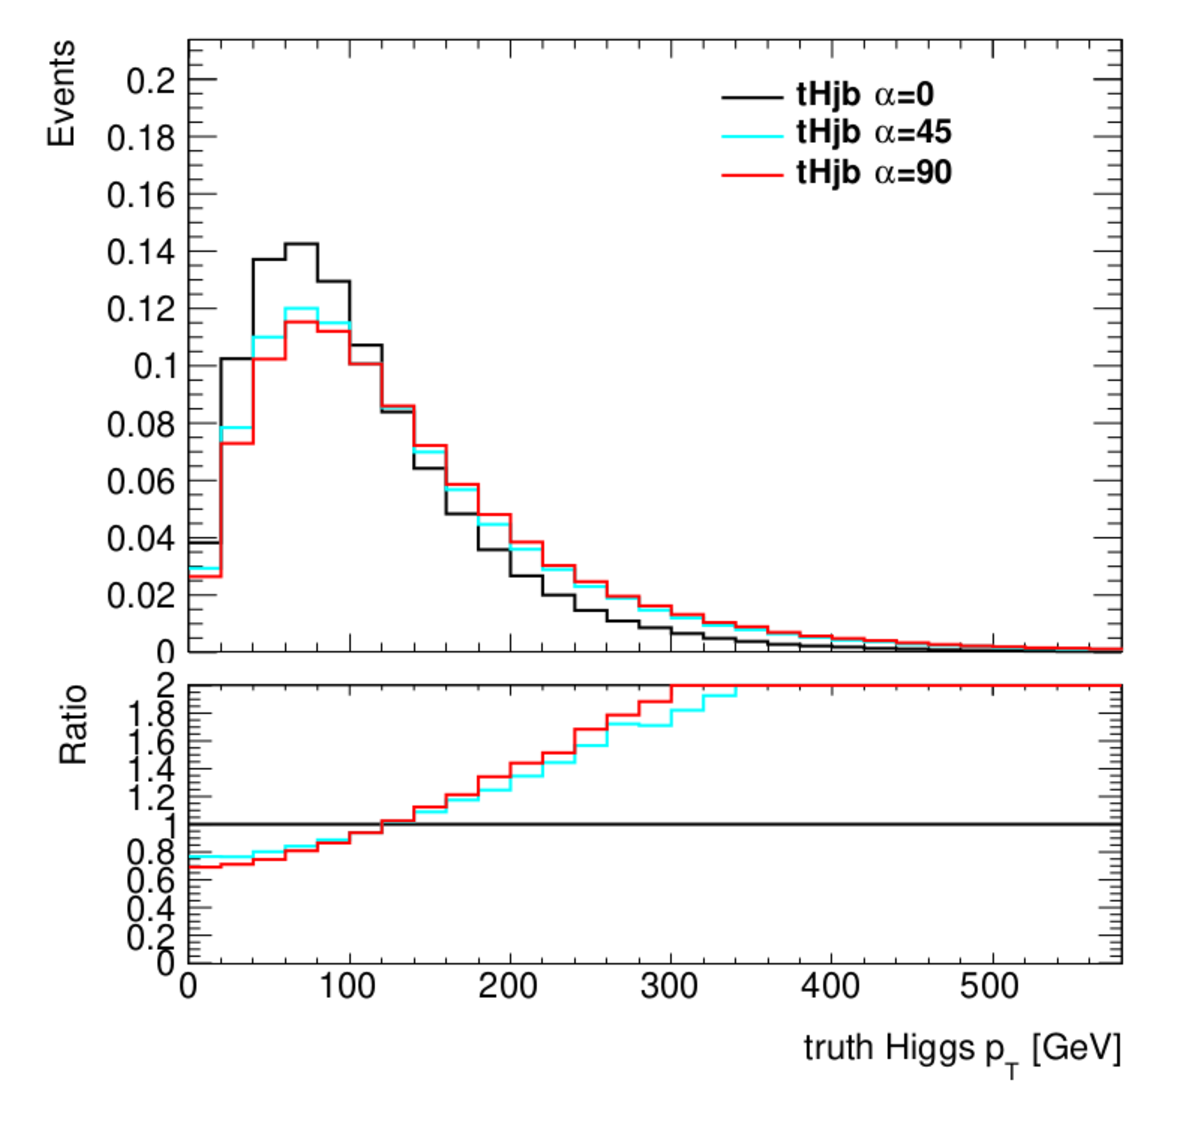
\includegraphics[width=0.35\textwidth]{figures/tthcp_chapter/observables/tHjb/c_H_pt.pdf}
      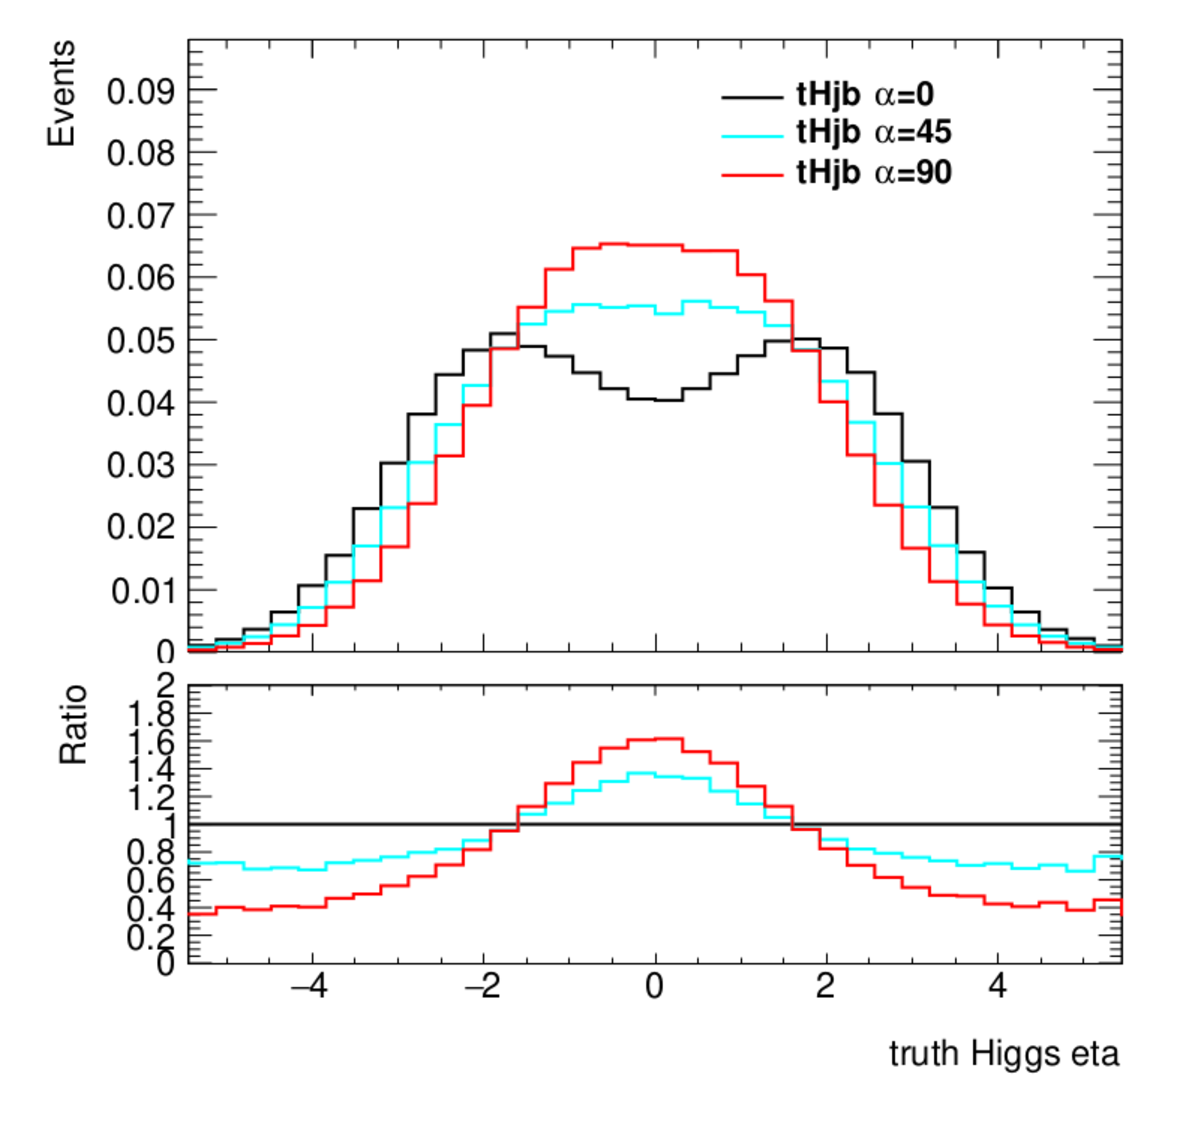
\includegraphics[width=0.35\textwidth]{figures/tthcp_chapter/observables/tHjb/c_H_eta.pdf}
    }
    \mbox{ 
      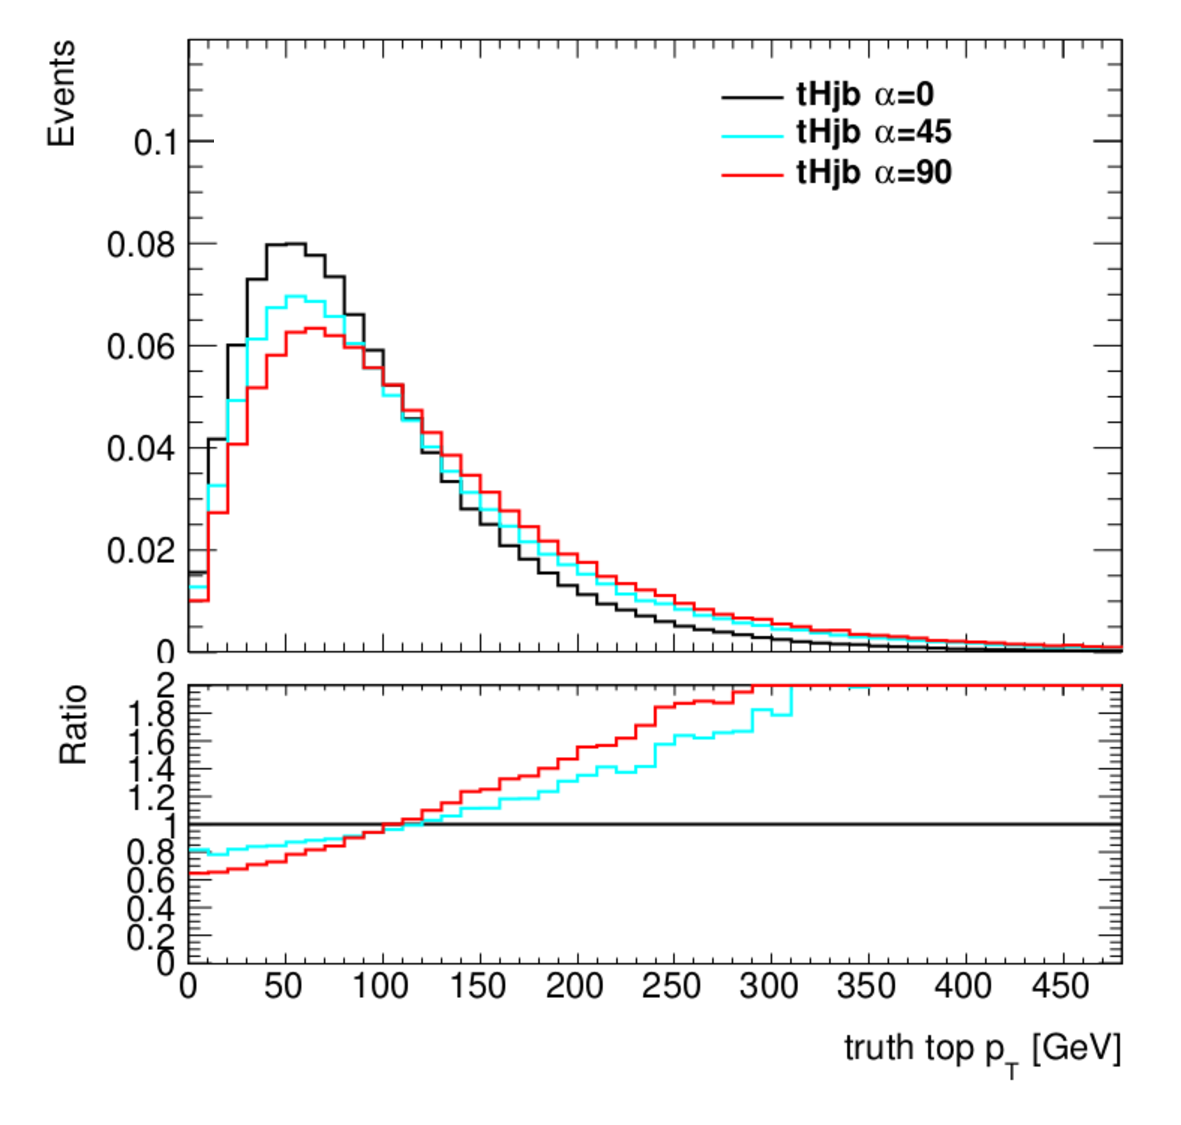
\includegraphics[width=0.35\textwidth]{figures/tthcp_chapter/observables/tHjb/c_t_pt.pdf}
      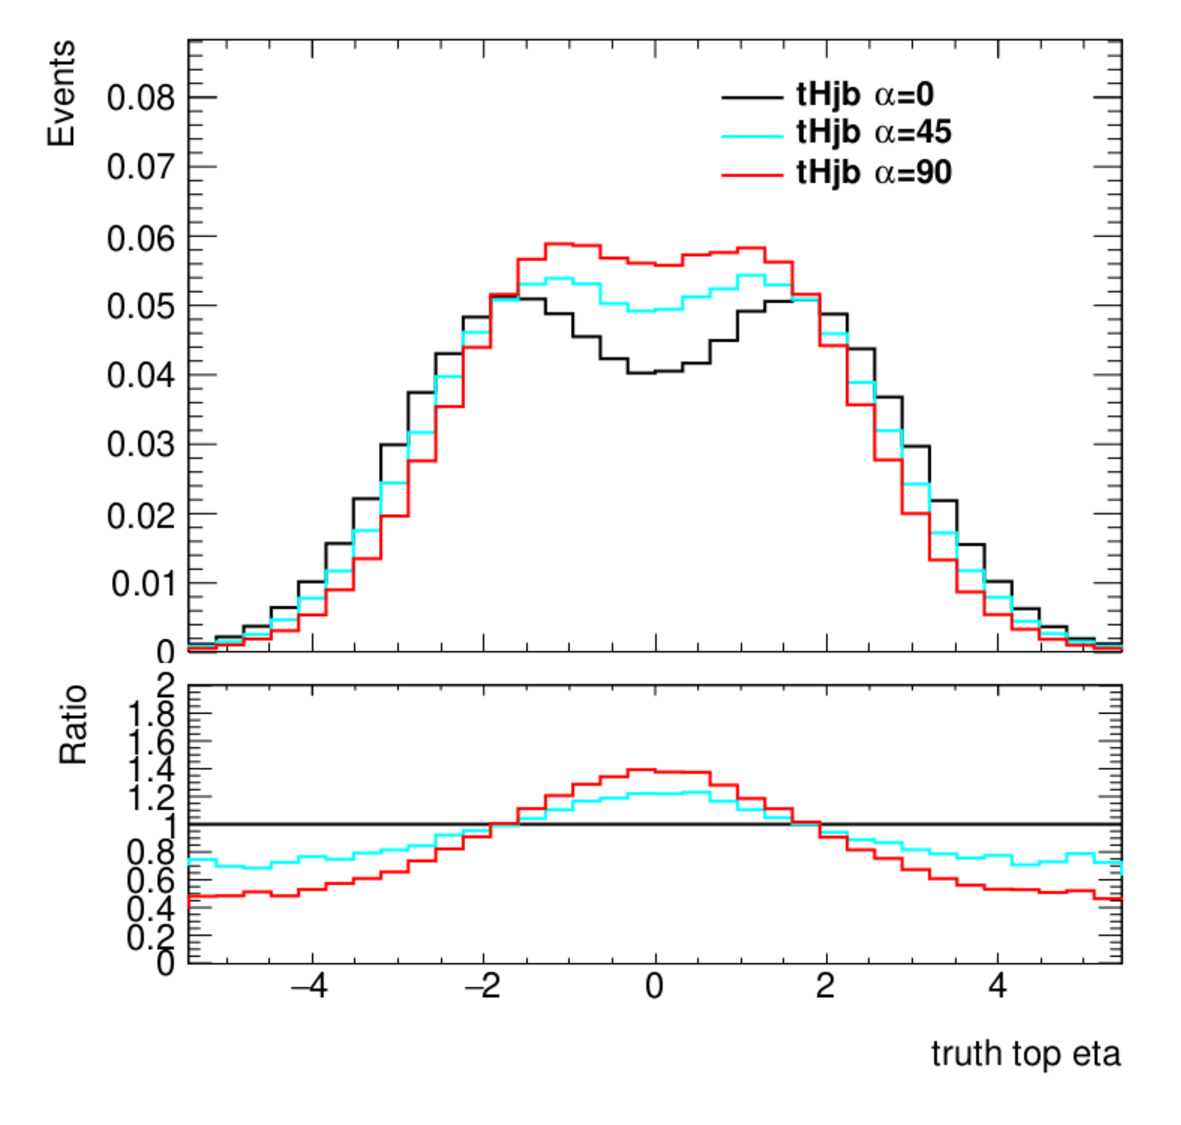
\includegraphics[width=0.35\textwidth]{figures/tthcp_chapter/observables/tHjb/c_t_eta.pdf}
    }
    \mbox{ 
      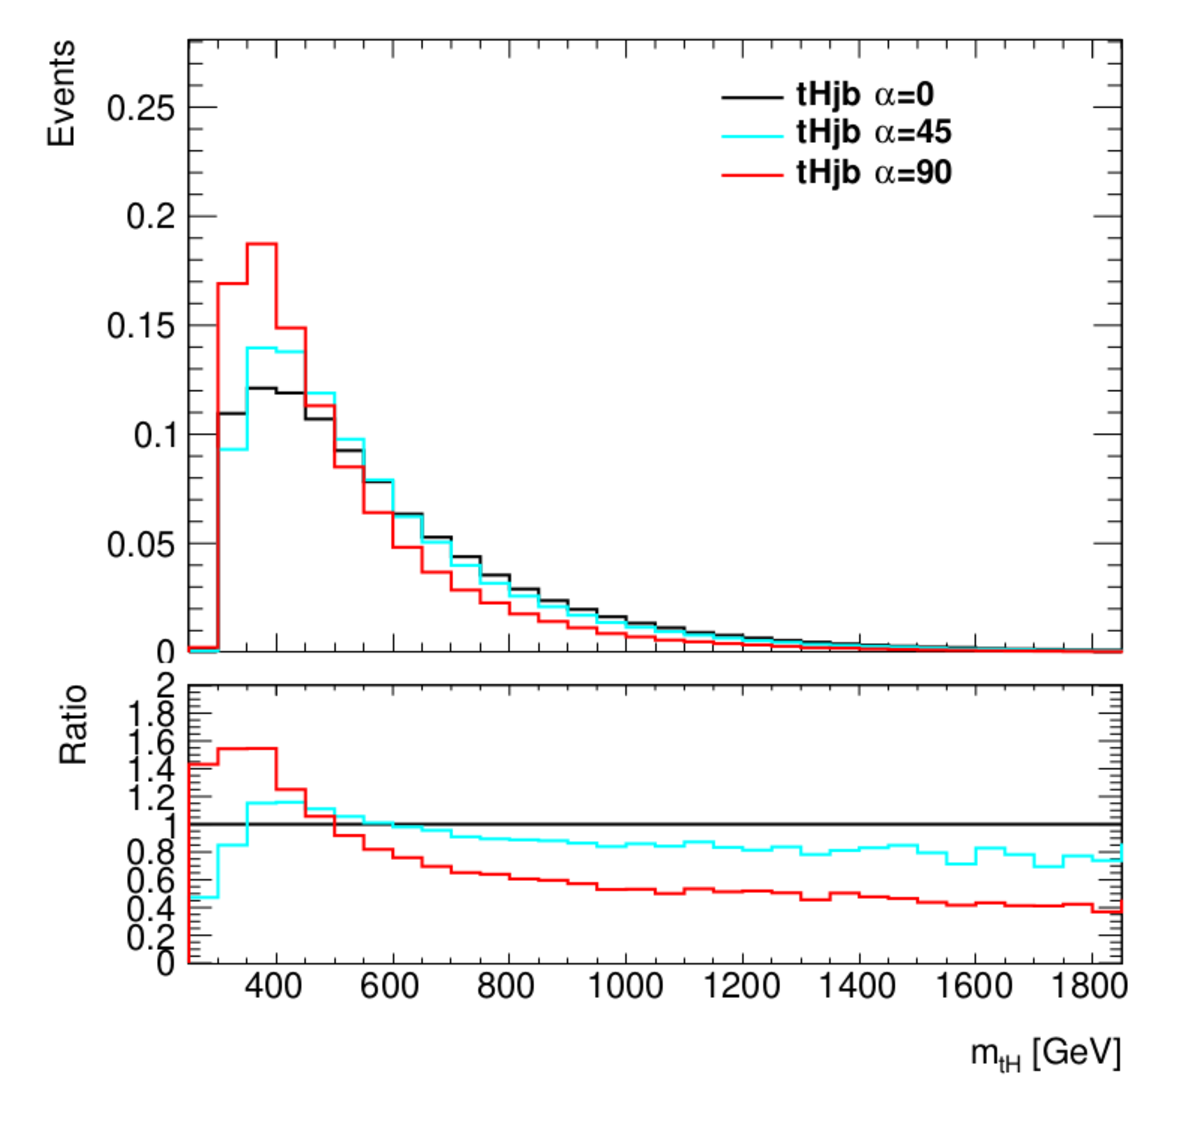
\includegraphics[width=0.35\textwidth]{figures/tthcp_chapter/observables/tHjb/c_tH_m.pdf}
    }
  \end{center}
  \caption{Truth-level distributions in $tHjb$ Monte Carlo of the Higgs boson $p_{T}$ and $\eta$ (top), angular separation between top and anti-top quarks (second row), top quark $p_{T}$ and $\eta$ (third row) and invariant mass of the top-Higgs system (bottom) for different values of the CP mixing angle $\alpha$.}
  \label{fig:tHjb_truth}
\end{figure}
\clearpage

\subsection{CPBDT}

Similar to the SBBDT case, two dedicated CPBDTs are trained using XGBoost, one in the hadronic preselection region and one in the leptonic preselection region. An alternative implementation of the BDT is developed using the Toolkit for Multivariate Analysis (TMVA) \cite{TMVA} and is discussed in Appendix \ref{app:TMVABDT}. Studies performed with the TMVA BDT helped guide the implementation of this BDT, including making the determination that only one dedicated CP-even vs CP-odd BDT was needed (rather than training for multiple $\alpha$ points) and the discovery of several useful high-level variables.

The signal samples are the CP-odd $ttH+tWH+tHjb$, added according to their expected cross-sections, while the background samples are the CP-even $ttH+tWH+tHjb$. 50\% of the signal and background samples are used for training, 25 \% are used for categorization, and 25\% are used for testing and significance evaluation.

For both the hadronic and leptonic CPBDTs, input variables chosen are:

\begin{itemize}
\item $p_{T}$ (again scaled by $m_{\gamma \gamma}$) and $\eta$ of the Higgs candidate
\item $p_{T}$, $\eta$, $\phi$ (with respect to the Higgs candidate), and BDT score of the first and second reconstructed tops. Due to its potential to be composed of fewer than three jets, the second top is referred to as the 'hybrid' top. In events where no hybrid top is reconstructed, a dummy value is passed to XGBoost.
\item Angles $\Delta\eta$ and $\Delta\phi$ between the two top candidates. If no second ('hybrid') top is reconstructed, a dummy value is passed to XGBoost.
\item The invariant mass of the top-Higgs system ($m_{t1H}$), and the invariant mass of the two-top system ($m_{t1hy}$). In the case where no second hybrid top is reconstructed, a dummy value is passed to XGBoost.
\item $H_{T} = \sum_\text{jet j} p^{j}_{T}$
\item The minimum $\Delta$R between a photon and a jet (out of all possible photon-jet pairs in the event)
\item The second-smallest $\Delta$R between a photon and a jet (out of all possible photon-jet pairs in the event)
\item Number of jets and number of $b$-jets in the event
\item Missing $E_{T}$ significance = $E_{T}^\text{miss}/\sqrt{H_{T}}$
\end{itemize}

The XGBoost BDT parameters are optimized by running the training 100 times with hyper-parameters selected according to a Bayesian minimization procedure \cite{skopt}. The integral of the Receiver Operating Curve (ROC AUC) is used as the optimization metric, evaluated on the validation set for each training. The ROC-AUC measures true-positives versus true-negatives, parameterized as a function of classifer threshold cuts: a completely random classifier has a ROC-AUC of 0.5, while a perfect classifier has a ROC-AUC of 1.0 \cite{ROC}. The ROC-AUC for the hadronic CPBDT is 0.7839, while the ROC-AUC for the leptonic BDT is 76.69.

Plots of the CPBDT input variables for the leptonic BDT are shown in figures \ref{fig:lepvbls1} -  \ref{fig:lepvbls3}, while plots of the hadronic CPBDT input variables are shown in figures \ref{fig:hadvbls1} -  \ref{fig:hadvbls3}.

\begin{figure}[htbp]
  \centering
  	\subfloat[Higgs candidate $p_{T}$ (GeV)]{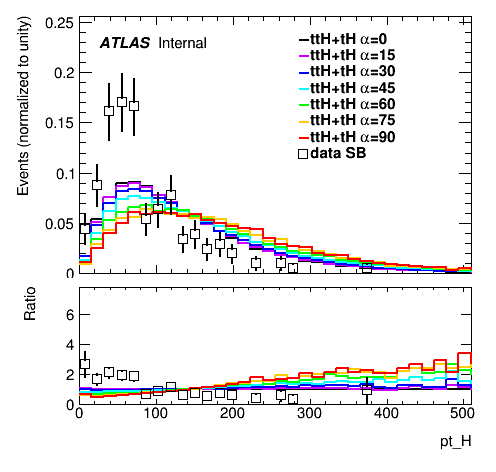
\includegraphics[width=0.31\textwidth]{figures/tthcp_chapter/categorization_xgb/lep-vbls/pt_H.png}}
	\subfloat[Higgs candidate $\eta$]{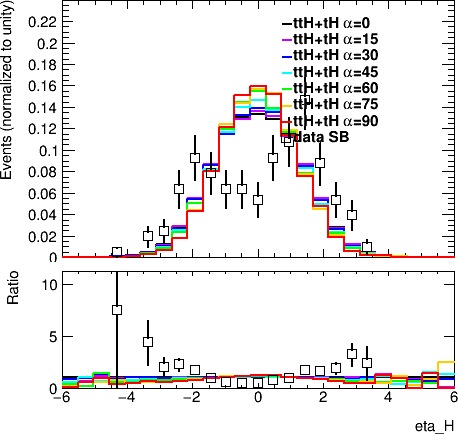
\includegraphics[width=0.31\textwidth]{figures/tthcp_chapter/categorization_xgb/lep-vbls/eta_H.png}} 
  	\subfloat[Top 1 $p_{T}$ (GeV)]{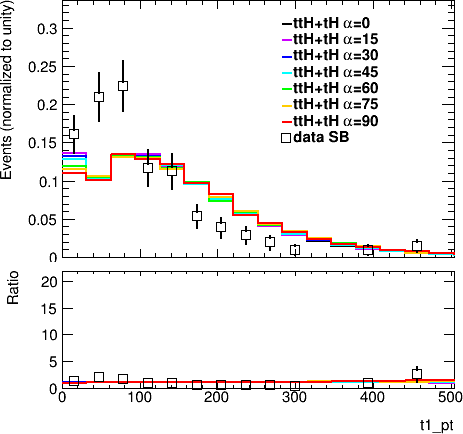
\includegraphics[width=0.31\textwidth]{figures/tthcp_chapter/categorization_xgb/lep-vbls/t1_pt.png}} \\
	\subfloat[Top 1 $\eta$]{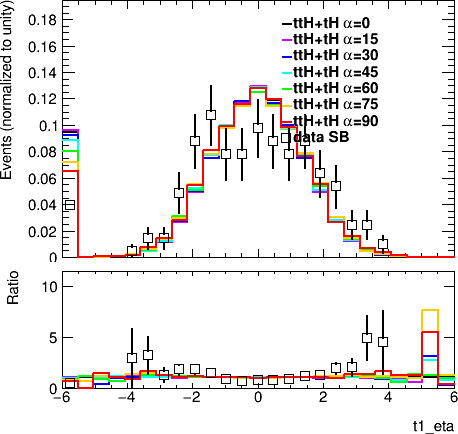
\includegraphics[width=0.31\textwidth]{figures/tthcp_chapter/categorization_xgb/lep-vbls/t1_eta.png}}
	\subfloat[Top 1 $\phi$]{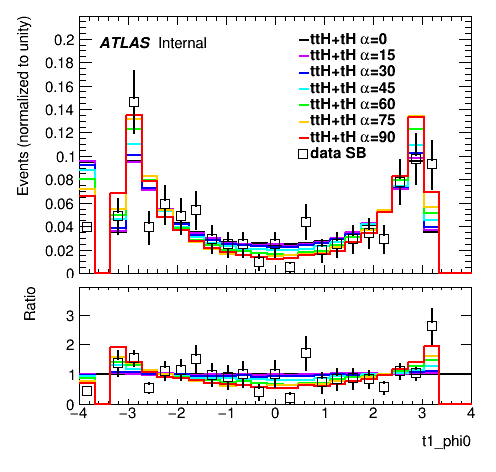
\includegraphics[width=0.31\textwidth]{figures/tthcp_chapter/categorization_xgb/lep-vbls/t1_phi0.png}} 
	\subfloat[Top 1 Reco BDT score]{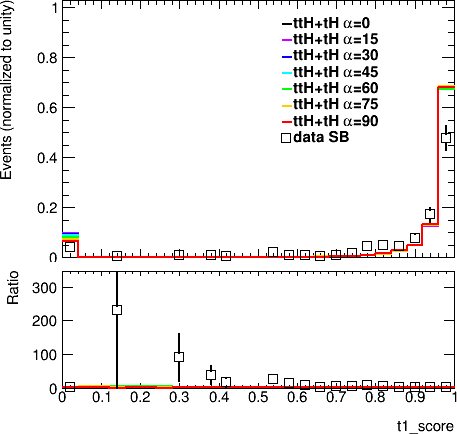
\includegraphics[width=0.31\textwidth]{figures/tthcp_chapter/categorization_xgb/lep-vbls/t1_score.png}}\\
  \caption{Leptonic BDT training variables. The top $\phi$ is calculated with respect to the Higgs candidate. The open squares indicate data in the NTI sideband region, which approximates the shape of the continuum background.}
  \label{fig:lepvbls1}
\end{figure}	
	
\begin{figure}[htbp]	 
  	\subfloat[Hybrid top 2 $p_{T}$ (GeV)]{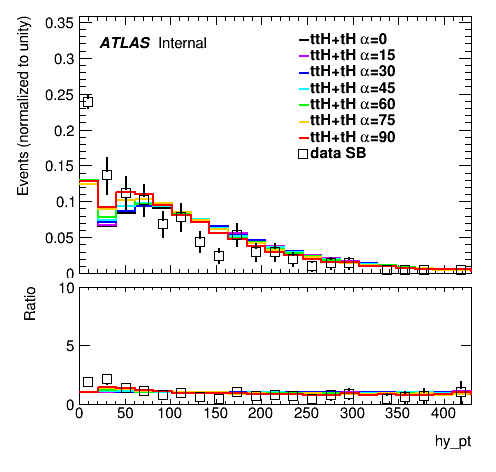
\includegraphics[width=0.32\textwidth]{figures/tthcp_chapter/categorization_xgb/lep-vbls/hy_pt.png}}
	\subfloat[Hybrid top 2 $\eta$]{\includegraphics[width=0.32\textwidth]{figures/tthcp_chapter/categorization_xgb/lep-vbls/hy_eta.png}}
	\subfloat[Hybrid top 2 $\phi$]{\includegraphics[width=0.32\textwidth]{figures/tthcp_chapter/categorization_xgb/lep-vbls/hy_phi0.png}} \\
	\subfloat[Hybrid top 2 Reco BDT score]{\includegraphics[width=0.32\textwidth]{figures/tthcp_chapter/categorization_xgb/lep-vbls/t2_score.png}}
  	\subfloat[$\Delta\eta_{t1t2}$]{\includegraphics[width=0.32\textwidth]{figures/tthcp_chapter/categorization_xgb/lep-vbls/delta_eta_t1hy.png}}
	\subfloat[$\Delta\phi_{t1t2}$]{\includegraphics[width=0.32\textwidth]{figures/tthcp_chapter/categorization_xgb/lep-vbls/delta_phi_t1hy.png}}  
  \caption{Leptonic BDT training variables. The top $\phi$ is calculated with respect to the Higgs candidate. The underflow bins in hybrid top $p_{T}$/$\eta$/ $\phi$ and $\Delta\eta_{t1t2}$/ $\Delta\phi_{t1t2}$ contain events where no second ('hybrid') top is reconstructed, while the underflow bin in the BDT score contains events with fewer than six jets (i.e., events with either no hybrid top or a hybrid top that is reconstructed using the remaining-jets method). The open squares indicate data in the NTI sideband region, which approximates the shape of the continuum background. }
  \label{fig:lepvbls2}
\end{figure}

\begin{figure}[htbp]
  \centering
  	\subfloat[$m_{t1H}$ (GeV)]{\includegraphics[width=0.31\textwidth]{figures/tthcp_chapter/categorization_xgb/lep-vbls/m_t1H.png}}
	\subfloat[$m_{t1hy}$ (GeV)]{\includegraphics[width=0.31\textwidth]{figures/tthcp_chapter/categorization_xgb/lep-vbls/m_t1hy.png}}
  	\subfloat[$n_\text{jets}$]{\includegraphics[width=0.31\textwidth]{figures/tthcp_chapter/categorization_xgb/lep-vbls/m_njet.png}}\\
	\subfloat[$n_\text{b-jets}$]{\includegraphics[width=0.31\textwidth]{figures/tthcp_chapter/categorization_xgb/lep-vbls/m_nbjet_fixed80.png}} 
	\subfloat[$H_{T}$ (GeV)]{\includegraphics[width=0.31\textwidth]{figures/tthcp_chapter/categorization_xgb/lep-vbls/m_HT.png}}
	\subfloat[Missing $E_{T}$ significance]{\includegraphics[width=0.31\textwidth]{figures/tthcp_chapter/categorization_xgb/lep-vbls/m_met_sig.png}}\\
  	\subfloat[$\Delta R_{min}^{\gamma j}$]{\includegraphics[width=0.31\textwidth]{figures/tthcp_chapter/categorization_xgb/lep-vbls/delta_Rmin_yj.png}}
  	\subfloat[$\Delta R_{min}^{\gamma j2}$]{\includegraphics[width=0.31\textwidth]{figures/tthcp_chapter/categorization_xgb/lep-vbls/delta_Rmin_yj2.png}}
  \caption{Leptonic BDT training variables. The underflow bins in $m_{t2H}$ and $m_{t1t2}$ contain events where no second ('hybrid') top is reconstructed. The open squares indicate data in the NTI sideband region, which approximates the continuum background shape. }  	
  \label{fig:lepvbls3}
\end{figure}

\clearpage

The XGBoost BDT parameters are optimized by running the training 100 times with hyper-parameters selected according to a Bayesian minimization procedure \cite{skopt}. The area under the ROC curve (ROC AUC) is evaluated on the validation set for each training, and the training that maximizes the ROC AUC is selected as optimal.

\begin{figure}[htbp]
  \centering
  	\subfloat[Higgs candidate $p_{T}$ (GeV)]{\includegraphics[width=0.31\textwidth]{figures/tthcp_chapter/categorization_xgb/had-vbls/pt_H.png}}
	\subfloat[Higgs candidate $\eta$]{\includegraphics[width=0.31\textwidth]{figures/tthcp_chapter/categorization_xgb/had-vbls/eta_H.png}} 
  	\subfloat[Top 1 $p_{T}$ (GeV)]{\includegraphics[width=0.31\textwidth]{figures/tthcp_chapter/categorization_xgb/had-vbls/t1_pt.png}} \\
	\subfloat[Top 1 $\eta$]{\includegraphics[width=0.31\textwidth]{figures/tthcp_chapter/categorization_xgb/had-vbls/t1_eta.png}}
	\subfloat[Top 1 $\phi$]{\includegraphics[width=0.31\textwidth]{figures/tthcp_chapter/categorization_xgb/had-vbls/t1_phi0.png}} 
	\subfloat[Top 1 Reco BDT score]{\includegraphics[width=0.31\textwidth]{figures/tthcp_chapter/categorization_xgb/had-vbls/t1_score.png}}\\ 
  \caption{Hadronic BDT training variables. The top $\phi$ is calculated with respect to the Higgs candidate. The open squares indicate data in the NTI sideband region, which approximates the shape of the continuum background. }
  \label{fig:hadvbls1}
\end{figure}


\begin{figure}[htbp]
  \centering
  	\subfloat[Hybrid top 2 $p_{T}$ (GeV)]{\includegraphics[width=0.32\textwidth]{figures/tthcp_chapter/categorization_xgb/had-vbls/hy_pt.png}}
	\subfloat[Hybrid top 2 $\eta$]{\includegraphics[width=0.32\textwidth]{figures/tthcp_chapter/categorization_xgb/had-vbls/hy_eta.png}}
	\subfloat[Hybrid top 2 $\phi$]{\includegraphics[width=0.32\textwidth]{figures/tthcp_chapter/categorization_xgb/had-vbls/hy_phi0.png}} \\
	\subfloat[Hybrid top 2 Reco BDT score]{\includegraphics[width=0.32\textwidth]{figures/tthcp_chapter/categorization_xgb/had-vbls/t2_score.png}}
  	\subfloat[$\Delta\eta_{t1t2}$]{\includegraphics[width=0.32\textwidth]{figures/tthcp_chapter/categorization_xgb/had-vbls/delta_eta_t1hy.png}}
	\subfloat[$\Delta\phi_{t1t2}$]{\includegraphics[width=0.32\textwidth]{figures/tthcp_chapter/categorization_xgb/had-vbls/delta_phi_t1hy.png}}  
  \caption{Hadronic BDT training variables. The top $\phi$ is calculated with respect to the Higgs candidate. The underflow bins in top $p_{T}$/$\eta$/ $\phi$ and $\Delta\eta_{t1t2}$/ $\Delta\phi_{t1t2}$ contain events where no second ('hybrid') top is reconstructed, while the underflow bin in the BDT score contains events with fewer than six jets (i.e., events with either no hybrid top or a hybrid top that is reconstructed using the remaining-jets method). The open squares indicate data in the NTI sideband region, which approximates the shape of the continuum background. }
  \label{fig:hadvbls2}
\end{figure}

\begin{figure}[htbp]
  \centering
  	\subfloat[$m_{t1H}$ (GeV)]{\includegraphics[width=0.31\textwidth]{figures/tthcp_chapter/categorization_xgb/had-vbls/m_t1H.png}}
	\subfloat[$m_{t1hy}$ (GeV)]{\includegraphics[width=0.31\textwidth]{figures/tthcp_chapter/categorization_xgb/had-vbls/m_t1hy.png}}
  	\subfloat[$n_\text{jets}$]{\includegraphics[width=0.31\textwidth]{figures/tthcp_chapter/categorization_xgb/had-vbls/m_njet.png}}\\
	\subfloat[$n_\text{b-jets}$]{\includegraphics[width=0.31\textwidth]{figures/tthcp_chapter/categorization_xgb/had-vbls/m_nbjet_fixed80.png}} 
	\subfloat[$H_{T}$ (GeV)]{\includegraphics[width=0.31\textwidth]{figures/tthcp_chapter/categorization_xgb/had-vbls/m_HT.png}}
	\subfloat[Missing $E_{T}$ significance]{\includegraphics[width=0.31\textwidth]{figures/tthcp_chapter/categorization_xgb/had-vbls/m_met_sig.png}}\\
  	\subfloat[$\Delta R_{min}^{\gamma j}$]{\includegraphics[width=0.31\textwidth]{figures/tthcp_chapter/categorization_xgb/had-vbls/delta_Rmin_yj.png}}
  	\subfloat[$\Delta R_{min}^{\gamma j2}$]{\includegraphics[width=0.31\textwidth]{figures/tthcp_chapter/categorization_xgb/had-vbls/delta_Rmin_yj2.png}}
  \caption{Hadronic BDT training variables. The underflow bins in $m_{t2H}$ and $m_{t1t2}$ contain events where no second ('hybrid') top is reconstructed. The open squares indicate data in the NTI sideband region, which approximates the continuum background shape. }  	
  \label{fig:hadvbls2}
\end{figure}

Plots of the CPBDT output score for both the hadronic and leptonic CPBDT are shown in Figure \ref{fig:cpscores}, while two-dimensional plots of CPBDT score versus SBBDT score for data in both the hadronic and leptonic regions are shown in Figures \ref{fig:2dbdthad} and \ref{fig:2dbdtlep}.

\begin{figure}[htbp]
  \centering
  	\subfloat[Hadronic]{\includegraphics[width=0.45\textwidth]{figures/tthcp_chapter/categorization_xgb/had-vbls/BDTG_cp.png}}
  	\subfloat[Leptonic]{\includegraphics[width=0.45\textwidth]{figures/tthcp_chapter/categorization_xgb/lep-vbls/BDTG_cp.png}}
  \caption{Hadronic and Leptonic CP BDT scores for $ttH$+$tHjb$+$tWH$, with relative weights according to their expected cross sections under various CP mixing scenarios.  The open squares show data in the NTI sideband region. }
  \label{fig:cpscores}
\end{figure}

\begin{figure}[htbp]
 \centering
  	\includegraphics[width=0.6\textwidth]{figures/tthcp_chapter/categorization_xgb/BDTdist_had_zero.pdf}
  \caption{Distribution of events from TI sidebands, CP even signal, and CP odd signal in the 2D background rejection BDT vs. CP BDT plane in the hadronic category are shown in full color, black, and red contours, respectively, along with 1D projections onto each BDT score. Inner (outer) contours contain 25\% (50\%) of signal events.}
  \label{fig:2dbdthad}
\end{figure}

\begin{figure}[htbp]
 \centering
  	\includegraphics[width=0.6\textwidth]{figures/tthcp_chapter/categorization_xgb/BDTdist_lep_zero.pdf}
  \caption{Distribution of events from TI sidebands, CP even signal, and CP odd signal in the 2D background rejection BDT vs. CP BDT plane  in the leptonic category are shown in full color, black, and red contours, respectively, along with 1D projections onto each BDT score. Inner (outer) contours contain 25\% (50\%) of signal events.}
  \label{fig:2dbdtlep}
\end{figure}


\subsection{Poisson Number-Counting Significance}
In order to determine the optimal categorization based on BDT score, two Poisson number-counting significance metrics are used.

In physics analyses such as those discussed in this dissertation, the probability of observing k events in a given region of phase space given an expected number of events $\lambda$ is modeled by a Poisson distribution:

\begin{equation}
P(k, \lambda) = \frac{\lambda^{k}e^{-\lambda}}{k!}
\end{equation}

To determine the compatibility of the observed number of events with a given signal hypothesis H vs the Standard Model, it is useful to define a test statistic called the Poisson Number-Counting Significance:

\begin{align}
\begin{aligned}
Z^{2} = -2 ln(\frac{P(S + B, S_{H} + B)}{P(S + B, S + B)}) \\
= 2(S + B) ln(\frac{(S + B)}{(S_{H} + B)} -2(S + B) + 2(S_{H} + B)
\end{aligned}
\end{align}

Where S and B are the Standard-Model expected signal and background and $S_{H}$ is the expected signal under hypothesis H.

Thus, the $ttH+tH$ Standard-Model number-counting significance (that is, the significance of observing the amount of $ttH+tWH+tHjb$ in analysis categories that is predicted by the Standard Model if, in fact, the signal process does not exist and the background-only "null hypothesis" is true) can be defined as:

\begin{align}
Z_{ttH+tH} = \sqrt{2((S+B)\ln(1+S/B)-S)}
\label{eq:ncztth}
\end{align}

and the CP-Odd number-counting significance as:

\begin{align}
Z_{CP}(90) = \sqrt{2(S_e + B)\ln(\frac{S_e+B}{S_o + B}) -2(S_e + B) + 2(S_o + B)}
\label{eq:nczcp}
\end{align}

where $S_{e}$ is the amount of signal expected if $\alpha = 0^{\circ}$ and $S_{o}$ is the amount of signal expected if $\alpha = 90^{\circ}$.

To determine the total significance for either of these metrics across a number of categories, the number-counting significances for each category are added in quadrature.

To estimate the number of continuum background events B in the diphoton mass signal region in each category (that is, $123$ GeV $< m_{\gamma\gamma} < 127$ GeV), a scaling method is applied to the NTI data control region in the mass sidebands (that is, $105$ GeV $< m_{\gamma\gamma} < 123$ GeV or $127$ GeV $< m_{\gamma\gamma} < 160$ GeV):

\begin{align}
\begin{aligned}
N(TI,sig) = N(NTI, SBs)\times \frac{N(TI, SBs)}{N(NTI, SBs)} \times \frac{N(NTI, sig)}{N(NTI, SBs)} \\
= N(NTI, SBs) \times f_{1} \times f_{2}
\end{aligned}
\end{align}

Where the scale-factors $f_{1}$ and $f_{2}$ are calculated separately using the hadronic and leptonic preselection regions. The combined scale factor, $f_{1} \times f_{2}$, is found to be 0.013 for the hadronic region and 0.016 for the leptonic region. 

In order to ensure that there is sufficient data to perform a likelihood fit, at least 0.8 continuum events (as modelled by scaled NTI sidebands) ar required in the $123$ GeV $< m_{\gamma\gamma} < 127$ GeV signal window in each category.

\subsection{2D Categorization}

To determine the categorization, a scan is performed across many different sets of category boundaries, calculating both $Z_{ttH+tH}$ and $Z_{CP}(90)$ on the validation set. Because the same categorization scheme does not optimize both metrics, a compromise scenario is constructed, for which $Z_{ttH+tH}$ is maximized while $Z_{CP}(90)$ is required to be no more than $0.15\sigma$ less than its maximal determined value. The brute-force scan, and this effect, is shown in figure \ref{fig:optimal}. The categories selected are given in table \ref{tab:boundaries}. The expected yield and purity in each category is given in Figure \ref{fig:nominalb}.

\begin{figure}[htbp]
 \centering
        \subfloat[Hadronic]{\includegraphics[width=0.42\textwidth]{figures/tthcp_chapter/categorization_xgb/had/Zcomp_had.png}}
        \subfloat[Leptonic]{\includegraphics[width=0.42\textwidth]{figures/tthcp_chapter/categorization_xgb/lep/Zcomp_lep.png}}
  \caption{$Z_{CP}$ vs. $Z_{ttH}$ for all sets of boundaries considered.}
  \label{fig:optimal}
\end{figure}

\begin{table}[ht]
\begin{center}
\begin{tabular}{lll}
Category & Bkg. Rej. BDT score & CP BDT score \\ \hline
1 & $\left[0 - 0.005\right]$ & $\left[0 - 0.90\right]$ \\
2 & $\left[0 - 0.005\right]$ & $\left[0.90 - 0.97\right]$ \\
3 & $\left[0 - 0.005\right]$ & $\left[0.97 - 1 \right]$ \\
4 & $\left[0.005 - 0.009\right]$ & $\left[0 - 0.88 \right]$ \\
5 & $\left[0.005 - 0.009\right]$ & $\left[0.88 - 0.96\right]$ \\
6 & $\left[0.005 - 0.009\right]$ & $\left[0.96 - 1\right]$ \\
7 & $\left[0.009 - 0.019\right]$ & $\left[0 - 0.84 \right]$ \\
8 & $\left[0.009 - 0.019\right]$ & $\left[0.84 - 0.96\right]$ \\
9 & $\left[0.009 - 0.019\right]$ & $\left[0.96 - 1\right]$ \\
10 & $\left[0.019 - 0.091\right]$ & $\left[0 - 0.61 \right]$ \\
11 & $\left[0.019 - 0.091 \right]$ & $\left[0.61 - 0.86\right]$ \\
12 & $\left[0.019 - 0.091 \right]$ & $\left[0.86 - 1\right]$ \\ \hline
13 & $\left[0 - 0.012\right]$ & $\left[0 - 0.91 \right]$ \\
14 & $\left[0 - 0.012 \right]$ & $\left[0.91 - 1\right]$ \\
15 & $\left[0.012 - 0.085\right]$ & $\left[0 - 0.82\right]$ \\
16 & $\left[0.012 - 0.085\right]$ & $\left[0.82 - 0.93 \right]$ \\
17 & $\left[0.012 - 0.085\right]$ & $\left[0.93 - 1\right]$ \\
18 & $\left[0.085 - 0.748\right]$ & $\left[0 - 0.72\right]$ \\
19 & $\left[0.085 - 0.748\right]$ & $\left[0.72 - 0.86\right]$ \\
20 & $\left[0.085 - 0.748\right]$ & $\left[0.86 - 1 \right]$ \\  \hline
\hline
\end{tabular}
\end{center}
\vspace{-0.5cm}
\caption{Category boundaries which optimize the Poisson number-counting rejection significance of the CP odd scenario in the 12 hadronic and 8 leptonic categories.}
\label{tab:boundaries}
\end{table}

\begin{figure}[htbp]
 \centering
        \subfloat[Event yield (CP even $ttH$)]{\includegraphics[width=0.42\textwidth]{figures/tthcp_chapter/categorization_xgb/cp_11p8_a0.png}}
        \subfloat[Purity (CP event $ttH$)]{\includegraphics[width=0.42\textwidth]{figures/tthcp_chapter/categorization_xgb/cp_11p8_purity_a0.png}} \\
        \subfloat[Event yield (CP odd $ttH$)]{\includegraphics[width=0.42\textwidth]{figures/tthcp_chapter/categorization_xgb/cp_11p8_a90.png}}
        \subfloat[Purity (CP odd $ttH$)]{\includegraphics[width=0.42\textwidth]{figures/tthcp_chapter/categorization_xgb/cp_11p8_purity_a90.png}}
  \caption{(Left) Event yields in the CP categories. Shown separately for $\alpha = 0^{\circ}$ and $\alpha = 90^{\circ}$. (Right) purity of the Higgs yield in each category for $\alpha = 0^{\circ}$ and $\alpha = 90^{\circ}$. Yields are calculated in the signal window $m_{\gamma\gamma}=125\pm2$ GeV.}
  \label{fig:nominalb}
\end{figure}

The background-only statistical uncertainty in a given category is given by:

\begin{align}
s = \frac{S}{Z_{ttH+tH}}
\label{eq:statunc}
\end{align}

It is also useful to define:

\begin{equation}
n_{s}(\alpha) = n_{ttH}^{SM} + n_{tWH}^{SM} + n_{tHjb}^{SM} - n_{ttH}(\alpha) - n_{tWH}(\alpha) - n_{tHjb}(\alpha)
\end{equation}

as an indication of the "signal" (i.e., difference between Standard-Model and alternative-$\alpha$ yield) in each category. 

\begin{figure}
\end{figure}

Using this, the effects of major systematics can be computed, ensuring they do not need to be accounted for at the categorization stage.The 100\% ggF yield uncertainty and the Parton Shower Uncertainty (calculated by subtracting the yield in each category using the Herwig Monte Carlo samples from the yield using the Pythia samples) are shown in Table \ref{tab:systs}- in all categories, it is clear that the statistical uncertainty dominates. This can be confirmed by plotting the number-counting rejection for the CP-odd category, $Z_{CP}(90^{\circ})$, both with and without systematics in figure \ref{fig:ncrej_syst}. 


\begin{table}[ht]
\begin{center}
\begin{tabular}{lllllll}
Category & $n_{s}(90^\circ)$ & $\delta$ & $n_{ggF}$ &PS (ttH)&PS (tWH)&PS (tHjb) \\ \hline 
1&-2.226&1.462&0.247&-0.157&0.008&0.01 \\ 
2&2.038&1.581&0.044&-0.049&-0.007&-0.005 \\ 
3&1.111&1.136&0.002&0.098&0&0 \\ 
4&-0.956&1.275&0.208&-0.039&-0.043&-0.038 \\ 
5&0.57&1.534&0.054&-0.008&-0.02&-0.006 \\ 
6&1.086&1.554&0.009&0.08&-0.005&-0.007 \\ 
7&-1.393&1.597&0.448&-0.053&-0.02&-0.014 \\
8&0.505&2.713&0.186&0.015&-0.01&-0.002 \\ 
9&1.287&2.623&0.021&0.094&0.007&-0.001 \\ 
10&-1.09&1.363&0.557&-0.003&0.019&-0.012 \\
11&-2.365&3.858&1.25&-0.053&-0.038&0.026 \\
12&2.33&7.86&0.6&0.007&-0.025&0.006 \\ \hline 
13&-0.835&1.398&0.001&-0.149&-0.024&-0.006 \\
14&2.542&1.64&0.001&0.156&-0.008&0.001 \\
15&-1.218&1.168&0.004&-0.089&-0.024&-0.011 \\
16&0.473&1.643&0&-0.015&-0.012&-0.014 \\
17&1.32&1.697&0.001&-0.036&0.001&0 \\
18&-0.899&1.082&0.008&-0.016&0.032&-0.027 \\
19&-0.284&1.627&0.008&-0.024&0.022&-0.01 \\ 
20&0.309&1.973&0.003&-0.014&-0.013&0.013 \\ \hline 
\hline
\end{tabular}
\end{center}
\vspace{-0.5cm}
\caption{Comparison of statistical uncertainty with key systematics and CP-Odd vs. SM separation in each category. PS indicates parton showering uncertainty, calculated by subtracting the yields from the Herwig and the Pythia Monte Carlo samples.}
\label{tab:systs}
\end{table}

\begin{figure}
  \centering
        \includegraphics[width=0.62\textwidth]{figures/tthcp_chapter/categorization_xgb/cp_11_syst.png}
  \caption{The impact of systematic uncertainties on the number counting limit. There is a small change of $0.3^\circ$ on the number-counting limit, thus indicating that systematics do no appreciably affect the categorization.}
  \label{fig:ncrej_syst}
\end{figure}


\begin{table}[ht]
\begin{center}
\begin{tabular}{ll}
Number-counting $ttH$ significance (if even)& $5.00\sigma$  \\
Number-counting $ttH$ significance (if odd)& $2.75\sigma$  \\
Number-counting $tHjb + tWH$ significance (if even)& 0.321$\sigma$  \\
Number-counting $tHjb+tWH$ significance (if odd)& $2.23\sigma$  \\ \hline
Number-counting CP-odd rejection & $3.02\sigma$ \\
Number-counting $\alpha=45^\circ$ rejection & $1.25\sigma$ \\ \hline
\hline
\end{tabular}
\end{center}
\vspace{-0.5cm}
\caption{Significance metrics for the full twenty-category CP BDT categorization, calculated using event yields in the signal $m_{\gamma\gamma}$ region $125\pm2$ GeV.}
\label{tab:sigs}
\end{table}
